%%%%%%%%%%%%%%%%%%%%%%%%%%%%%%%%%%%%%%
% This is the name of the style file.
%%%%%%%%%%%%%%%%%%%%%%%%%%%%%%%%%%%%%%
%
% phd  -> for a PhD dissertation
% ms   -> for an MS thesis
% If both phd and ms are used then phd will overide.  If none are used,
% then ms will be active by default.
%
% cpyr -> generate a copyright page
% lof  -> generate List of Figures
% lot  -> generate List of Tables
\documentclass[ms,cpyr,lof,lot]{uathesis}
%
%%%%%%%%%%%%%%%%%%%%%%%%%%%%%%%%
% List of any packages you use.
%%%%%%%%%%%%%%%%%%%%%%%%%%%%%%%%
%

\usepackage[nounderscore]{syntax}
\usepackage{listings}
\usepackage{textcomp}
\usepackage{setspace}
\usepackage{amsmath}
\usepackage{amssymb}
\usepackage{epsfig}
\usepackage{graphicx}
%\usepackage[colorlinks=false]{hyperref}
\usepackage[chapter]{algorithm}
\usepackage{algpseudocode}
\usepackage[linewidth=1pt]{mdframed}
%\usepackage{changebar}
\usepackage{url}
%\usepackage{environ}
%\usepackage{inconsolata}
\usepackage{subcaption}
\usepackage[margin=1cm]{caption}
\usepackage{xcolor}


\lstdefinelanguage{steve}
{
	morecomment=[l][\color{gray}\textit]{//}
}

\lstset{
		language=steve,
		basicstyle=\ttfamily\singlespacing\small,
	    emph={
	    	layout, int, uint, decoder, extract, var, else, if, exact_table, event, match, case, while, miss, break, continue, Port, return, def, in\_port, in\_phys\_port, egress, reflow, controller, all, timeout,  flood
	    },
	    emph=[2]{ start, as, requires, advance },
	    emph=[3]
	    {
	    	output, decode, goto, drop, set, write, clear, raise, insert, into, remove, from,
	    },
	    emphstyle={\color{blue}\textbf},
	    emphstyle=[2]{\color{green}\textbf},
	    emphstyle=[3]{\color{red}},
	    frame=single,
	    tabsize=2
}

%%%%%%%%%%%%%%%%%%%%%%%%%%%%%%%%%%
%%   Dealing with grammar style

\renewcommand{\syntleft}{$\langle$\ttfamily\itshape}
\renewcommand{\syntright}{$\rangle$}

\renewcommand{\litleft}{\ttfamily}
\renewcommand{\litright}{}

%\renewcommand{\ulitleft}{\ttfamily}
%\renewcommand{\ulitright}{}

%%%%%%%%%%%%%%%%%%%%%%%%%%%%%%%%%%%%

\graphicspath{ {./images/} }

\newenvironment{minip}
  {\noindent
   \begin{minipage}{\textwidth}\begin{flushleft}
   \singlespace
  }
  {\end{flushleft}\end{minipage}\vspace{\baselineskip}}

\setlength{\grammarparsep}{1pt}

\newenvironment{codepage}
  {\noindent
   \begin{minipage}{\textwidth}
   \singlespace
  }
  {\end{minipage}\vspace{\baselineskip}}

%\noindent\begin{minipage}{\linewidth}
%\begin{grammar}
%\singlespace
%
%
%\end{grammar}
%\end{minipage}


%
%%%%%%%%%%%%%%%%%%%%%%%%%%%%%%%%%%
% List of definitions you define.
%%%%%%%%%%%%%%%%%%%%%%%%%%%%%%%%%%
%
\def\ds{\displaystyle}
\def\E{\epsilon}

%%%%%%%%%%%%%%%%%%%%
% Defining inline grammar macros
%%%%%%%%%%%%%%%%%%%%
\def\la{\textlangle{}}
\def\ra{\textrangle{}}
\def\mn{\text{-}}
\newcommand\grddd[4]{\la\textit{\texttt{#1}} \mn \textit{\texttt{#2}} \mn \textit{\texttt{#3}} \mn \textit{\texttt{#4}}\ra}
\newcommand\grdd[3]{\la\textit{\texttt{#1}} \mn \textit{\texttt{#2}} \mn \textit{\texttt{#3}}\ra}
\newcommand\grd[2]{\la\textit{\texttt{#1}} \mn \textit{\texttt{#2}}\ra}
\newcommand\gr[1]{\la\textit{\texttt{#1}}\ra}

%

\title{Steve - A Programming Language for Packet Processing}
\author{Hoang Nguyen}
\conferraldate{May}{2016}

%The following commands specify the names and titles of people that
%will appear on the signature page.
%
%These four will always be needed.
\advisor{Andrew Sutton}
\chair{Timothy O'Neil}
\collegedean{John Green}
\gradschdean{Chand Midha}

%For a PhD dissertation, specify a coadvisor and three committee
%members, or four committee members only.  For an MS thesis use either
%one coadvisor or one faculty reader, not both.
%
%Typical commands for a PhD dissertation (uncomment only 4).

% FIXME: This isn't right. I think we require a committee of 3 in the
% department.

\committee{Name of 1st Comm Member}
\committee{Name of 2nd Comm Member}
\committee{Name of 3rd Comm Member}
\committee{Name of 4th Comm Member}

%Typical commands for an MS thesis (uncomment only 1).
%\coadvisor{Andrew Sutton}
\facreader{NAME 1}
\facreader{NAME 2}

\begin{document}
\maketitle
\chapter{INTRODUCTION} \label{ch:intro}

% FIXME: The introduction needs to flow. Don't break it up into this kind of
% question and answer dialog, and don't skimp on motivation. Take this guy's
% PhD thesis as an example:
%
% http://www.cs.colostate.edu/~christos/thesis/chp1.pdf
%
% It's a little more detailed than you'll need, but it's a good example of
% how to motivate the problem and organize both the solution and your
% contributions.

% FIXME: Use \emph to emphasize terms, not boldface.

The Internet is nowadays ubiquitous with everyday life. In the last twenty
years,
the industry has rapidly evolved to incorporate all kinds of new Internet
services:
cloud services, web services, Internet of Things, etc. As the world grows
more reliant on services provided over a network, so must the network evolve.

The backbone of all networks is the \emph{switch}. The term switch here is not used to specifically mean a Layer 2 forwarding device. but rather to mean any device capable of making forwarding decisions across multiple layers of the OSI stack \cite{osi_model}. The term switch thus incorporates bridges, routers, content switches, etc.
Unfortunately, modern switches suffer from a number of issues which make them difficult to use in an industry where networks are so essential.

Conventional switches are complex and unscalable because many of these devices are designed to deal only with very specific sets of well-known protocols and use cases. A router, for example, may be reconfigured with new forwarding rules, but it will never be anything other than a router. The behavior simply cannot change, making these devices very rigid.
Though these devices can be reconfigured, network administrators are often forced to do so through clunky command line interfaces. Additionally, because they may only be reconfigured within a limited use case, they cannot easily adapt to dynamic changes in network traffic and load.

In order to bypass this inflexibility, it must be possible to implement network functions (routing, firewalls, NAT, etc) through intelligent networking applications written in software.
These intelligent applications must be capable of automatically adapting to changing network conditions by modifying switch behavior to optimize forwarding decisions, throughput, resource consumption, etc.
There must also exist a switch which is capable of installing and running this software.
There is a strong desire in the industry to have such switches to meet constantly changing needs in ways that a network administrator could not.

This is the promise of \emph{software-defined networking} (SDN). 
SDN modifies two major elements of a conventional network switch: the data plane and the control plane. The \emph{data plane}, sometimes called the \emph{forwarding plane}, is the element which is responsible for forwarding packets between ports on the device. The control plane is the element which learns and configures the forwarding logic used by the data plane. It is also capable of processing packets which the data plane cannot.

The Open Network
Foundation (ONF) defines SDN as the ``separation of the network control
plane from the forwarding [data] plane'' \cite{onf_sdn_def}.
Either of these components may then be implemented in regular software.
The goal of SDN architectures is to provide highly programmable, scalable, and 
efficient network functions in software.

The conventional control plane is replaced by a software application known as a \emph{controller} (software control plane).
This controller then serves as the intelligent network application which manages the switch's behavior. Alternatively, it may serve as an interface so that multiple network applications may manage the switch.
One of the more interesting differences is that
the software controller may be run on any machine, completely separate from its data plane.
It may then perform distributed control over multiple data planes by communicating via network messages.
The most widely adopted standard for this communication is OpenFlow
\cite{openflow_spec}.
Because the software controller may be run on any machine,
any programmer can write regular software for common operating
systems and processors to control the behavior of their networking device.

The software control plane is only the first step. The next
step is the \emph{programmable data plane} which may be implemented
in either specialized hardware or software. 
A programmable data plane provides
two key benefits that the software control plane cannot: low-latency,
customizable packet processing and \emph{protocol independence}.

%In the control and data plane relationship,
%the control plane is smart but slow, while the data plane is fast yet dumb.
%That is,
%the control plane can perform general purpose computing but communicating with
%it has high latency. The data plane, on the other hand, is the fast path for
%packet processing.
%It has very limited computing power, but can process packets at a low latency.
%As programmable data planes evolve and support more flexible instruction sets,
%communicating with the control plane becomes less necessary.

The software control plane supports general purpose computing using heavyweight
processors. However, general purpose computing is slow and communicating
with the control plane over a network using messages is even slower.
Data planes, on the other hand, can process packets incredibly fast since
they are designed for this single role, but do not necessarily support
the full range of general purpose operations.
If data planes could support more kinds of computation, then they can rely less
on
slow control planes, and delegate only under the more extreme circumstances.

Protocol independence means that a networking device is not required, by default, to support
a suite of well-known protocols (ethernet, IPv4, TCP, etc).
Rather than relying on specialized hardware or firmware tailored towards
parsing/decoding
these protocols, the data plane supports processors
and generic instructions that can be used to decode and operate on
any header and field.
This allows users to support their own protocols in addition to
supporting well-known protocols. This makes the data plane scalable, that is, it
can adapt to new headers easily.

%Intelligence implies that a machine or program is capable of performing a myriad of general purpose computations which one might find on normal CPU. 
%Consider a router for example. These machines are said to be intelligent because of the algorithms they use to route traffic across multiple networks. They may even support intelligent load and content balancing. But are they really intelligent compared to what modern computers are capable of? 
%
%Of course not. Modern devices use specialized hardware to process network traffic at maximum speeds, but as a trade-off, they lose the ability to perform general purpose computation that would support implementing intelligent network functions. Why is this so important?
%
%Network traffic can carry data which is completely inaccessible to many modern switches because they are incapable of processing everything. Consider how powerful it would be if any application could be installed on a network switch.




%Modern routers and switches provide the backbone for the Internet.
%These modern devices implement two fundamental components in their firmware: the
%\emph{data plane} and the \emph{control plane}. A control plane can be thought of as the brains of a network device, whereas the
%data plane is the brawn.
%
%The data plane is responsible for processing packet content and and moving them across the right ports.
%It makes fast forwarding decisions by using lookup tables to determine
%where a packet is sent. When it does
%not know how to handle a packet, it sends it to the control plane.
%
%A control plane manages its data plane.
%It is responsible for installing forwarding logic for a network device and is
%capable of learning new forwarding behaviors in response to unexpected packets.
%It does this by modifying the lookup tables used by the data plane.
%Together, the control and data plane implement \emph{network functions}, i.e.
%switching, NAT, firewall, etc.
%
%This model continues to be the most popular for switch development.
%However,
%this conventional type of networking has become too rigid, unscalable, and
%proprietary to support evolving technologies. 
%
%Defining network functionality in firmware is inherently inflexible.
%Firmware is architecture-dependent, difficult to write, and challenging to
%update
%regularly.
%Conventional switches are unscalable because they must deal with most or all
%common protocol headers.
%With dozens of common protocols now, and potentially dozens more in the future,
%it becomes evident that this model cannot last forever.
%Additionally, many devices are black boxes,
%only exposing an interface designed by the vendor,
%making them difficult to customize for enterprises with special needs.
%By extension, these black box devices force any network functions
%defined over them to be extremely architecture dependent.
%Due to these issues and others, a new paradigm for networking was created. 
%
%This new paradigm
%is called \textit{software-defined networking} (SDN). 

\section{Motivation: A Language for Programming SDN Devices}

In order to pursue programmable SDN devices, there must be a language to write
programs that process packets and define network functions. 
A number of language solutions arise here.
Some attempt to solve this problem by providing APIs for existing programming
languages (specifically C).
Others attempt to produce domain-specific languages (DSLs) for SDN devices.

The focus of this thesis is one such DSL, \emph{Steve}, a language for the safe
and
efficient specification of packet processing and network functions 
for programmable SDN switches. DSL provide one key benefit that low-level
languages cannot: safety.

A network program must be safe to execute more than anything else.
Network programs, especially those running on high-traffic devices, must not
crash due to logical mistakes or unnoticed undefined behaviors.
At best, this produces expensive network downtime; at worst, this
opens the way for security vulnerabilities on the device: 
denial of service attacks, buffer overflows, etc.

Typical packet processing programs are written in low-level languages, most
commonly C. These C programs usually work with data plane programming APIs such
as Open Data Plane (ODP) \cite{odp_webpage} and the Data Plane Programming Kit
(DPDK) \cite{dpdk_webpage}. Unfortunately, programming network devices in C can be prone
to errors stemming from buffer and resource management. 
These issues are compounded by the fact C is a general
purpose language not tailored towards packet processing, thus the burden of
safety
is left to the programmer, with no compiler to double check their code.
Specifically, C programs risks errors such as:

\begin{itemize}
\item accessing memory outside the bounds of a packet buffer or within a
constrained
region of memory,

\item writing bytes which exceed a constrained subset of the packet
resulting in a buffer overflow (i.e. writing new bytes into a header field
but exceeding the size of that field),

\item buffer underflow when not writing enough bytes when modifying
a field,

\item using a field in an operation that is not supported by its
range of values,

\item non-terminating cycles in program logic (infinite loops
triggered by a single packet),

\item incorrect assumptions about decoding state. That is, a programmer using
a field which they have not extracted yet.
\end{itemize}

Programmers using C for SDN applications are also burdened with management of
device resources. Specifically, a C programmer must manage:

\begin{itemize}
\item memory. The programmer must manage their own buffers for holding packet
data and packet meta data. This opens the opportunity for accidental
memory leakage.

\item ports. The programmer is responsible for receiving, reading, and
forwarding
through ports. This process should be decoupled from the packet processing logic
for modularity. A packet processing application should be architecture
independent
whereas port management is a architecture dependent problem.
\end{itemize}

% Low-level packet processing code can be very light on easy to understand
% abstraction and very heavy on gritty implementation details. The programmer
% should be focusing on high-level abstractions; concepts such as: what fields
%are
% needed, what operations must be performed on these fields, conditional
%decision
% making, packet classification, etc. Instead, they are worried about the many
% common ailments of writing in low-level code.
%
% The programmer must deal with resource allocation and management. They must
%deal
% with allocating their own buffers for storing packets and by extension must
%deal
% with de-allocating those buffers. This type of resource management is prone to
% accidental memory leakage, especially in C. Memory leakage of gigabytes of
%data
% will quickly bring a system down.
%
% The programmer must directly manage ports. They are also responsible for
% manually receiving, reading, and sending packets on those ports. This is code
%is
% common to all packet processing applications. The programmer should not be
% burdened with this kind of common code when writing a packet processor.
%
% When working with packet headers, the programmer must manually work with raw
% arrays of bytes. The burden of decoding fields from byte arrays and
%interpreting
% the value of those fields is shifted onto the programmer. Manual decoding can
%be
% a painful process on its own. It is prone to error, particularly off-by-N
% errors. When reinterpreting those bytes into header data structures, the
%result
% can be disastrous if the bytes are wrong or the data structure is wrong.
%Moving
% or copying those bytes around is particularly prone to buffer overflows.
%
% A number of other common problems come up when working in low-level code.
% Undefined behavior from reading past the end of packet buffers can be one.
% Performing operations on null pointers, invalid pointers, or uninitialized
% memory is another.
%
% Steve and its runtime, Flowpath, attempt to remedy most of these problems. The
% objective is to abstract many of these low-level details. Instead, the
% programmer only focuses on the high-level abstractions. Specifically, the
%Steve
% language focuses the programmer on writing the packet processing pipeline and
% makes the grittier details opaque

\section{Motivation: Control and Data Plane Latency}

In addition to tackling the issue of a safe language, 
Steve also aims to take a new approach towards the troublesome
control and data plane communication that many other SDN
approaches have adopted.
The SDN abstract model using distributed/centralized control
planes to manage data planes has its flaws.
As mentioned earlier, communicating with a distributed control plane is slow.
The trade-off is that it allows for control over an
entire network.

A non-distributed control plane, on the other hand, has much
better performance.
It can exist on the
same hardware as the data plane and has little communication latency
because the two processes may communicate directly through an application
binary interface (ABI).
This model is considerably more effective for simple network functions.
Steve targets this model of non-distributed control.
The programming model for a control and data plane on the same device
is essentially basic event-driven programming (EDP).

The data plane raises events when it needs something from the control plane.
The control plane catches these events with special handlers and modifies the
forwarding logic accordingly.
A free benefit of this model is that a single language like Steve may
be used to define both control and data plane elements for a given 
device. 
 
\section{The Steve Programming Language}

The Steve programming language was designed to solve the problem of safe and efficient programming of SDN devices.
Steve is used for writing applications that define packet processing
and network functions on SDN devices.
It is protocol independent, strongly-typed,
and declarative.

Steve provides the mechanisms for defining \emph{packet
processing pipelines}, the core component used by a data plane
to process packet content and make forwarding decisions.
It also provides the ability to define \emph{event handlers} --
control plane functions which process unexpected packets and
modify the data plane when necessary.

\subsection{Packet Processing Pipelines}

The packet processing pipeline is a data plane algorithm that
uses multiple, smaller processing stages to decode packet content and make
forwarding decisions.
The Steve pipeline is a generalization
of the pipeline model defined by OpenFlow \cite{openflow_spec}.
Steve provides high-level language features for specifying
stages in this pipeline and how these stages connect.
Specifically, Steve allows for the definition of:

\textbf{Header Structures}.
A programmer may define the structure of any protocol header using an abstract
mechanism known as a \emph{layout}.
A layout specifies what fields are in a header, the lengths of those fields,
and types for those fields.

\textbf{Decoders}. Decoders are pipeline stages used to extract 
fields from a packet header. 
They conform to user-defined layouts, making them flexible enough
to deal with any protocol header.

%
% Steve allows the user to program special functions decoders
% which are used for decoding and extract fields from a header. Decoders allow
%the
% user to specify which fields they need. Decoders do not require that a user
% extract all fields if they do not need those fields. The user is not required
%to
% manually extract the bytes associated with a field. Instead, the user gives a
% field name from the header layout they defined, and the language generates the
% code for them.

\textbf{Flow tables}.
Flow tables are pipeline stages responsible for the majority of forwarding logic.
In networking, a \emph{flow} is a group of packets from a source to one 
or more  destinations. In order to facilitate these flows, Steve uses \emph{flow tables} (an OpenFlow inspired abstraction). 
A flow table is a dynamic
decision table which classifies packets into groups (flows) using
decision rules (known as \emph{flow entries}).
Packets which are part of the same flow have a common set of \emph{actions}
applied to them.

\textbf{Actions}. Actions provide a way to modify a packet's fields, add/remove
flow entries from tables, and forward/drop packets. Steve actions are a
generalization
of OpenFlow's instructions and actions.

\textbf{Pipeline Composition}. A Steve pipeline is a composition of two kinds of
stages: decoders and flow tables.
Steve provides languages features for describing how these stages are linked
together. It also provides safety guarantees on the pipeline.

\subsection{Event Handling and Control}

The pipeline may raise events to the control plane when
it cannot handle a packet. Steve allows for the definition of
\emph{event handlers} -- control plane functions which deal
with these special circumstances.
Unlike the pipeline, event handlers can execute a wider range of
operations that are too slow for a data plane such as:
logging, flow table modification, C library calls, etc.

\subsection{General Purpose Features}

Though Steve is an SDN language, it also supports a number of general purpose
features. 
Steve supports functions, variables, arithmetic, branching, 
looping and a foreign function interface which may be used to call linked C 
library functions.

\section{Contribution: A Language for Defining Safe Pipelines}

The Steve language provides a type and constraints system to ensure the safety
of all Steve-defined packet operations and pipelines.
In addition, Steve uses an optimizing compiler to ensure efficient code
generation
and a runtime environment to abstract hardware resources (ports, memory, etc).

\subsection{Type Safety}

Steve is a statically-typed language. The compiler performs additional work to
enforce strict safety guarantees so that runtime checks can be avoided as much
as possible.

The Steve type system ensures that operations on header fields are valid and
well-defined. 
To reduce errors related to working with fields as byte buffers, Steve allows
for the representation of fields as arbitrary precision, signed or unsigned
integers.
Implicit integer conversions can be applied to these fields where necessary.
Conversions prevent field modification from ever underflowing or overflowing.

Steve does not support pointer types, meaning that the programmer is never
concerned with null or invalid pointer addresses. Instead, Steve supports
reference
types which are guaranteed to refer to initialized memory.

%\begin{enumerate}
%\item the representation of fields as
%arbitrary precision, signed or unsigned integers, (as long as they
%are multiples of 8). This allows the programmer to avoid using arrays of bytes
%to represent fields.
%
%\item logical and arithmetic expressions which are type checked
%to ensure no undefined behavior happens (e.g. shifting by negative values,
%adding to a boolean, etc).
%
%\item implicit conversions can be applied where necessary (e.g. integer size
%promotion, unsigned to signed conversions, etc).
%
%\item buffer overflow/underflow prevention. 
%Writing a new value into a header field \textit{never} causes accidental
%buffer overflows. The Steve compiler uses implicit conversions to guarantee
%that
%the size of the new value fits exactly into the byte width of a field. If the
%new value is represented in less bytes than the size of field, it gets extended
%to fit. Values that are too large get truncated.
%\end{enumerate}


% Specifically, the Steve language aims to avoid:
%
% \begin{itemize}
% \item accessing memory outside the bounds of a packet buffer,
%
% \item writing bytes which exceed a contrained subset of the packet
% resulting in a buffer overflow (i.e. writing new bytes into a header field
% but exceeding the size of that field),
%
% \item buffer underflow resulting from not writing enough bytes when modifying
% a field,
%
% \item using the value of a field in an operation that is not supported by its
% range of value,
%
% \item non-terminating cycles of decoders and table matchings (an infinite loop
% of packet processing),
%
% \item incorrect assumptions about decoding state. That is, a programmer using
% a field which they have not extracted yet.
% \end{itemize}

\subsection{Pipeline Constraints System}

The Steve compiler ensures certain guarantees about the correctness of a Steve
pipeline. Steve pipelines may be represented as directed acyclic graphs. The
Steve compiler performs analysis on this graph to enforce the following
constraints.

\begin{enumerate}
\item Fields that have not been extracted by a decoder cannot be used. 

\item The traversal of a packet through a pipeline is always a linear
progression. That is, a packet may never enter a non-terminating cycle
of decoders and tables.
\end{enumerate}

\subsection{Resource Safety}

Steve never requires the user to heap allocate resources. The majority of
allocation is done on the stack, ensuring Steve applications are free of
memory leakage and faster (as heap allocation tends to be slow).

Steve relies on its runtime environment, Freeflow \cite{freeflow_software}, 
to manage system resources such as
ports, packet reading, and packet buffer allocations.
This decouples the logic of system resource management from the packet
processing logic.

\subsection{Efficiency}

%Steve's programmable decoders provide the user the chance at certain
%optimizations. Steve allows the user to specify exactly which fields from a
%header they want extracted rather than forcing them to extract the entire
%thing.

High-level abstractions tend to produce performance penalties in exchange
for safety. The Steve compiler tries to reduce this penalty as much as possible.
The Steve compiler generates LLVM intermediate representation (IR) code
\cite{llvm_webpage}. The LLVM IR optimizing compiler is able to produce 
code equivalent to C programs. It also provides benefits such as
function inlining, peephole optimizations, etc.

Steve may also customize the LLVM compiler to produce
specialized instructions that are optimized for the architecture running
the application. This would be future work.

\section{Contribution: Modules For Freeflow Switches}

In order to validate that our language abstractions work, the Steve compiler builds modules (dynamic link libraries (DLL))
loaded by the Freeflow virtual machine (FFVM). The compiler currently targets an x86 architecture,
but can be adapted to target other platforms as well.

Freeflow is a virtual machine (VM) that also serves as the Steve runtime
environment \cite{freeflow_software}.
FFVM abstracts underlying switch
hardware and services and exposes them through an interoperable ABI.
Freeflow is a VM in the similar sense that Java Virtual Machine (JVM) is a VM. Targeting the VM ABI allows high-level applications to avoid generating architecture dependent code and optimizations.

FFVM may also be considered a software data plane.
A Steve module is designed to program FFVM's data plane pipeline by providing
flow table configuration, flow table entries, and packet decoders.
The module also instantiates the control plane for FFVM with the appropriate
event handlers.

\section{Thesis Overview}

This thesis is organized as follows. Chapter \ref{ch:related} describes similar
works in the field of SDN and SDN programming languages. It also provides a
background into SDN and the different approaches Steve takes to other languages
of its kind.

Chapter \ref{ch:pipeline_model} describes the components of Steve abstract machine. It explains the abstract model for packet processing pipelines and event handling.

Chapter \ref{ch:tutorial} describes the Steve programming language and how it is used to writing network functions.
Sample networking applications are also presented in
this chapter. These same samples are presented again in Appendix
\ref{ap:steve_programs}.

Chapter \ref{ch:limits} elaborates on pipeline safety guarantees and how they are enforced
as well as providing the proofs. It also provides explanations about other 
limitations of the language and why they exist.

Appendix \ref{ch:users_guide} serves as a reference
manual which includes semantic, grammar, and typing rules for the language.
This reference manual may be helpful to refer to when confused about a
Steve code example.

Chapter \ref{ch:flowpath} describes the interface which must be exposed by the switch or software running the switch. To validate this approach, this chapter also summarizes Freeflow, a virtual data plane which exposes this interface to Steve \cite{freeflow_software}. It also describes the interface which a Steve application exposes to the switch.

Chapter \ref{ch:experiments} provides experiments using sample Steve
applications. Pcap files are run through Steve applications to measure the data
rate and raw packet rate that each application is capable of running at on a
Linux machine.

Chapter \ref{ch:conclusion} details future work for Steve and provides concluding remarks about the project.
\chapter{BACKGROUND RELATED WORK}
\label{ch:related}

\section{Background}
\label{rel:openflow}

Software-defined networking aims to provide programmable network functions,
network management, and forwarding logic to modern networks that need more
than conventional switches.
Much of the work on the development of technologies for SDN is targeted at or 
inspired by OpenFlow: a specification describing the general architecture of SDN 
switches and the protocol that allows them to be remotely observed and controlled 
\cite{openflow_spec}. 

The key parts of the OpenFlow switch architecture, depicted in Figure \ref{fg:openflow_switch}, are a packet 
processing pipeline, an external software controller which sends and receives
OpenFlow messages, and ports. 

\begin{figure}[ht]
\centering
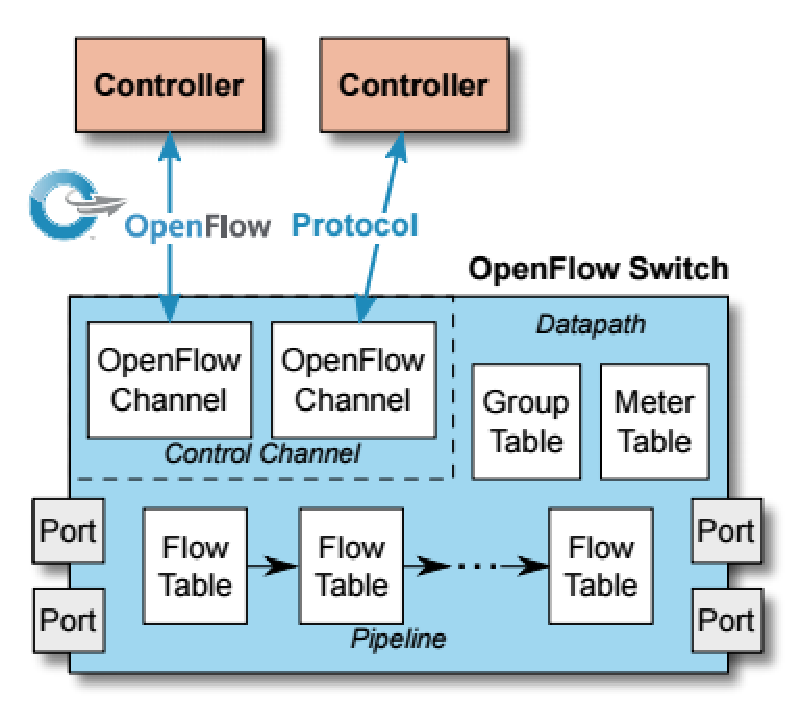
\includegraphics[scale=.5]{openflow}
\caption{The openflow switch architecture is made up of ports, a pipeline,
and an external controller which uses OpenFlow messages to communicate. (Image Source: \cite{openflow_spec})}
\label{fg:openflow_switch}
\end{figure}

This is the architecture that most SDN researchers and vendors have focused on.
Though OpenFlow is widely accepted and has driven the majority of SDN research,
it has its flaws.
OpenFlow's model places too much emphasis on the external software controller
and not enough focus on data plane elements (pipeline and ports).
OpenFlow focuses on non-programmable switch processors, making it too
constricting for Steve, which targets a programmable data plane.
Additionally, OpenFlow artificially constrains SDN evolution with its
unscalable, protocol-dependent pipeline model, instruction set, and message format.

Research into Steve used OpenFlow as a guide post for what an abstract
packet processing machine might look like and what language features may be
necessary to support such a machine. However, by no means did this research
strictly adhere to OpenFlow principles or semantics.

The primary concept Steve takes from OpenFlow is the pipeline processing model.
An OpenFlow pipeline is defined as a sequence
of one or more \textit{flow tables} and a \textit{group table} which handle
packet lookups, decision making, and forwarding.

The Steve pipeline has two key difference.
The first difference is that
Steve's pipeline is protocol independent, whereas OpenFlow specifies a limited set of
supported protocol fields known as OXM fields.
Because Steve is protocol independent, its
pipeline model must contain a series of programmable decoders to extract fields
from user-specified header structures. 
OpenFlow does not mention decoding because
implementation is usually left to the vendor.
For protocol dependent architectures, this is
usually done with specialized hardware.

The second difference are the actions used to modify the packet.
Steve flattens the instruction+action design of OpenFlow into
just actions. It also provides action extensions to manipulate flow tables
which OpenFlow does not. Additionally, Steve does away with the
strict and limiting action set limitation OpenFlow enforces.
Instead, Steve allows for any arbitrary list of actions to be applied
to a packet. 

Additionally, Steve does away with OpenFlow controllers. 
Steve focuses on network functions that do not require distributed control.
Though the OpenFlow model provides
the benefit of supporting distributed control, sending messages
over a network is simply too slow.
Therefore, Steve chooses to leverage the power of the control plane which
resides on the same switch as the data plane.

%The abstract SDN switch proposed by OpenFlow is not completely adopted by
%the Freeflow runtime. Specifically, the remote OpenFlow controller was
%removed from the Freeflow switch model. It is not desirable to remote configure
%a switch for basic reactive programs. Sending messages to a controller through
%a wire is a prohibitively high-latency operation.
%Instead of communicating with a remote controller via messages, Freeflow uses an 
%internal (non-distributed) controller which executes Steve event handlers. 
%However, Steve is still capable of decoding OpenFlow messages like any other protocol
%if there is a need for a distributed controller.

%An OpenFlow pipeline is defined as a sequence
%of one or more \textit{flow tables} and a \textit{group table} which handle
%packet lookups, decision making, and forwarding. Steve's packet processing pipeline differs from the traditional OpenFlow
%semantics in a number of ways. First,
%Steve provides language features for a user to create flow tables and define
%their flow entries, but does not yet support group tables.
%
%Second, a Steve pipeline has more than \textit{just} flow tables. Steve
%pipelines will also have \textit{decoders} which may be interleaved between
%tables. Decoders define how fields get decoded (or parsed) and extracted. In
%most switches, decoding is handled by specialized hardware that deal with
%well-known headers. OpenFlow only supports certain fields from these headers,
%known as OXM fields. However, the Freeflow data plane is
%protocol oblivious, knowing nothing about any specific headers; therefore
%decoding must be an explicit user-defined stage of the pipeline. By extension,
%Steve does not, by default, support these OXM fields either.

%Third, the semantics for packet handling using an external controller are different. An OpenFlow controller is software used to control an OpenFlow switch. It will handle ``exceptional events'' such as inserting,
%removing, and updating flow entries or processing packets which the pipeline
%could not. However, Steve and Flowpath do not use nor expect an external
%OpenFlow controller nor do they use OpenFlow messages to communicate with that
%controller.

%Steve and Flowpath attempt to reduce the role of the controller. Controller
%functions, which would typically handle exceptional cases (such as table
%manipulation and un-handled packets), can be written in Steve using special
%event handler functions. These event handlers are executed by the data plane
%on a special internal Flowpath ``controller'' thread rather than relying on an
%external controller.

\section{Early Steve Work}

Once people decided that programmable switch components were valuable,
they needed languages to program their controllers and data planes.
However, due to the sensitive nature of network applications, the program must be provably safe.

Early research into the Steve language focused on the correctness of packet
header definitions, safe packet access, and pipeline definitions.
Casey, et al, described the semantic constraints,
structural constraints (including buffer and view abstractions used by decoders), and 
safe access properties needed when working with packet buffers.
The Arbiter Framework was an early language implementation that checked the correctness of data paths (pipelines) and ensured that they did not violate the 
capabilities of switches they ran on.
\cite{arbiter}.

\section{SDN Programming Languages}

Many other projects have tackles the idea of an SDN programming language.
These languages may be further categorized into languages that program or configure
data plane elements, and languages which program the control plane or controller.

Languages which target the data plane all have the common idea of a pipeline.
These languages typically provide syntax packet decoding rules, table configuration,
and packet manipulation.
Controller languages tend to focus more on high-level, distributed control
of networks, designing network topology, and setting up forwarding policies
for an entire network.

Steve is unique in that it provides features for programming the data plane
and defines the reactive elements (i.e. event handlers) of the controller. However, since Steve
does not work with distributed control, it shares very little similarity with 
controller programming languages.

\subsection{SDN Data Plane Programming and Configuration Languages} \label{rel:p4}

P4 is the most popular protocol oblivious (independent) language for pipeline specification
 \cite{p4_spec, p4_spec2, p42014}.
P4 specifies a pipeline of programmable parsers (equivalent to Steve decoders) followed
by a series of match+action
tables (equivalent to flow tables). Parsing state is stored in a data structure
called a ``parsed representation.''

Huawei's Protocol-Oblivious Forwarding (POF) \cite{pof_fis, pof, pof_impl} provides a
low-level, assembly-like, instruction set for POF SDN switches. 
The POF programming model uses metadata as a ``scratch pad'' for parsing fields,
requiring that the programmer represent fields as generic \textit{\{offset, length\}} pairs, 
known as "search keys". The POF pipeline is a series of match tables which are also
responsible for decoding the fields they match on.

NetASM is an intermediate representation language for programmable data planes
\cite{shahbaz2015netasm}. It aims to solve the same issues as POF, but also provides a language that is target/device independent.

Steve is inspired by parts of P4 and POF, but also attempts to
fill in their weaknesses. 
Steve's pipeline specification syntax is similar to P4.
P4 high-level, abstract syntax is easy to write and understand. 
In contrast POF's instruction set (POF-FIS) \cite{pof_fis} is too
concrete, difficult to comprehend, and has no additional language
abstractions to ensure program safety.
POF search keys are particularly error prone because its not easy
for a programmer count field offsets manually.

However, Steve's abstract pipeline model is closer to POF's.
Steve decoders are placed between tables so fields are only decoded
as needed. This is similar to how POF tables extract their own fields.
Similarly, Steve uses POF's search key format for representing extracted fields, but the compiler generates the keys rather than the programmer. Steve adopts the POF decoding model.
The benefit of POF's decoding model is full control over what is or is not
extracted. 
That is, it allows the programmer to only decode a subset of fields within the header.
P4, on the other hand, extracts all header fields up-front, which is wastes 
valuable processing time if those fields are not needed.




%Essentially, fields only get extracted as they are needed, right before matching
%against a given table.

%Steve is a language for modifying the packet processing and forwarding functionality of a data plane. Steve is \textit{protocol oblivious}, meaning it does not by default
%know of any well-known network protocols (IPv4, IPv6, TCP, etc). Instead, it
%provides language features for programmers to deal with any protocol, making the
%language more scalable for future protocols. Other SDN languages are pursuing
%these idea as well.
%
%The P4 language \cite{p4_spec, p4_spec2, p42014} is another high-level language for
%defining protocol oblivious packet processing pipelines. It is probably the
%most widely adopted SDN language. P4 allows users to define packet headers,
%packet parsers and
%match+action tables (which are equivalent to OpenFlow flow tables). Parsers are
%used to extract entire headers and store them in a "parsed representation"
%before entering pipeline processing. When the packet enters the pipeline,
%match+action tables match against fields in the parsed representation and
%perform actions on matched packets.
%
%Protocol-Oblivious Forwarding (POF) \cite{pof_fis, pof, pof_impl} is another
%project also tackling the problem of protocol oblivious pipeline processing. POF
%is a very low-level, assembly-like, instruction set. The POF instruction
%set gives the programmer very fine-grained control of which fields get parsed.
%The POF programming model uses metadata as a "scratch pad" for parsing fields,
%requiring that the
%programmer represent fields as generic \{offset, length\} pairs, known as
%"search keys". When performing table matching, a programmer specifies
%an array of these search keys to match against the flow table.
%Essentially, fields only get extracted as they are needed, right before matching
%against a given table.
%
%POF also supports additional actions that allow the data plane to manipulate
%flow tables. This includes adding, removing, and updating flow
%entries. Though these actions are traditionally left up to the controller, they
%are useful because they reduce the load on the controller and provide
%flexibility to the data plane. This feature is notably absent from other SDN
%languages.
%
%The POF instruction set is difficult to write in and does not have the safety
%guarantees of a higher level language. The programmer is burdened with the
%error-prone task of parsing by manually specifying which bits comprise a fields.
%A high level language compiling into POF instructions would thus be ideal.
%
%Steve tries to take the best of both worlds. Steve can define decoding functions
%similar to P4 parsers, with the added benefit of allowing the programmer to only
%extract the fields they need, reducing the amount of time needed to parse
%overall. The \{offset, length\} pairs describing each field get generated by the
%Steve compiler rather than being manually written by the programmer, thus
%reducing
%the risk for error. Steve decoders may also be interleaved between tables,
%meaning fields can be extracted, as needed, right before table matching like
%POF. Like P4,
%Steve decoding can also happen all at once "up-front," before any table
%matching.
%It is up to the programmer to decide which is better. This makes Steve
%decoders a little more robust than either P4 or POF.
%
%Steve supports high-level definition of flow tables (or match+action tables in
%P4). Additionally, Steve also allows the programmer to define flow entries. This
%means the match field values and actions for each flow entry can be expressed
%within the language, allowing the Steve compiler to ensure safety and
%correctness guarantees over them. For example, adding a flow entry that causes
%an infinite loop is always prevented. This task is normally left up to the
%controller during runtime, which can be slow. Steve also supports instructions
%for adding and removing these flow entries from tables like POF.
%
%Unlike P4 and POF, Steve is not \textit{just} an SDN specific language; it is an
%extension to a general purpose language. It thus supports features like
%functions, function calls, lexical scoping, loops, conditional statements, and
%local/global variables. Steve also has support for types, arithmetic
%expressions, and comparison expressions. On top of that, it automatically links
%against the C Runtime Library, supports calls to external functions, and may be
%statically or dynamically linked against any library.
%
%Admittedly, P4 is a more mature language than Steve. P4 supports things like
%meters, variable sized fields, table matching methods (Steve only supports exact
%matching), and certain actions that Steve does not. P4 can also target more
%platforms than Steve, which currently only compiles into modules for Freeflow.
%POF also supports certain actions and table matching methods that Steve does not
%currently support.

\subsection{Data Plane Programming Libraries}
\label{rel:odp}

Data Plane Development Kit (DPDK) by Intel are software libraries in C for improving packet processing speeds on Intel processors and NICs \cite{dpdk_webpage}. DPDK provides a single platform (Intel processors) for performing all packet processing tasks, thus eliminating the need for specialized hardware.

Open Data Plane (ODP) is an open source API in C for developing data plane applications \cite{odp_webpage}. ODP provides application portability by providing a common set of APIs across multiple platforms and instruction set architectures.

\subsection{SDN Controller Programming Languages} \label{rel:frenetic}

The Frenetic project has produced a family of network programming
languages. Frenetic \cite{foster2011frenetic, foster2013frenetic} and Pyretic \cite{modularpyretic} are sister languages
that use SQL-like queries to classify packets and support a library for describing
packet forwarding policies over a collection of network switches. The goal is to
abstract away the difficulties of programming a centralized SDN controller.
NetCore is similarly a language for
generating classifiers from those policies \cite{monsanto2012netcore}. 
NetKAT does is similar to NetCore except it uses Kleene algebra \cite{kozen2014netkat, anderson2014netkat} to prove the correctness of its policies.

\section{Packet Parsers and Header Specifications}

Steve requires that a user specify the structure of their header.
Some early DSLs focused on binary header specification languages which inspired Steve syntax \cite{binpac, packet_types, datascript}.
Gibb, et al. described the design principles for parsing fields using header specifications
\cite{parser2013gibb}. Steve decoders may be described as a non-streaming programmable parsers. 
Some other examples of programmable packet parsers are Kangaroo \cite{kangaroo} and Berkley Packet Filter \cite{bpf1993mccanne}.

\section{Freeflow}
\label{rel:freeflow}

Freeflow is an SDN software switch architecture developed
by Flowgrammable \cite{freeflow_software}. The Freeflow virtual machine (FFVM) 
provides a programmable, protocol oblivious, software data plane that 
supports multi-tenancy. Steve is
designed to generate code targeting the FFVM runtime environment. A Freeflow data 
plane loads Steve applications which act as its control plane and programs its packet processing pipeline.

\section{Open vSwitch}
\label{rel:vswitch}

Open vSwitch is another SDN virtual, software switch which supports programmatic extensions \cite{ovs_man_page, ovs2009extending, ovs2013}. Open vSwitch was designed to work in virtual environments and runs on the hypervisor. It provides a high-level command line interface for re-configuring switches \cite{ovs_man_page}.



\chapter{THE PACKET PIPELINE PROCESSING MODEL} \label{pipeline_model}

A packet comes into a data plane via an ingress port. This packet must go through a series of processing stages where it is analysed, modified, and ultimately forwarded out through an egress port. These processing steps are what is known as a \textbf{pipeline}.

The Steve programming language allows programmers to define their own pipeline applications. In the Steve processing model a pipeline is a composition of two types of processing stages: decoding stages and table matching stages. Each stage performs a set of operations on a packet, known as actions, and decides where to move the packet next based on certain conditions that the packet meets. A packet can be moved to another processing stage or it can be sent out of the pipeline.

The pipeline is thus a state machine. Each processing stage denotes a state in the machine. Each state has a set of conditions which, when met, causes the packet to transition states. This can be represented as a graph where each processing stage is a node on the graph and each state transition is an edge connecting stages. This is a valuable property as it allows the Steve programming language to analyse these pipelines and enforce certain logical, safety, and correctness guarantees about a user-defined pipeline.

Steve pipelines follow a run-to-complete model of execution. Once a packet enters the pipeline, each processing stage is consecutively applied to the packet until the programmer decides to forward or drop the packet.

\section{Decoding Stage} \label{decoder_desc}

When a packet is received on its ingress port, it is a chunk of raw, uninterpreted data. Before a packet can be processed and routed, its headers and fields must be decoded and extracted so that meaningful decisions can be made about what to do with the packet. The decoding stage is responsible for ensuring this happens.

Steve allows for programmers to specify \textit{how} and \textit{which} fields are extracted from packet headers. In other paradigms, the \textit{entire} packet is decoded from start to finish; all headers and all fields are extracted, then all fields are saved. This is what is considered a \textbf{full decode}. After this full decode, the decision making process on the packet begins using those saved fields. However, this method is inherently inefficient. Only certain fields and headers within a packet are ever really needed during the forwarding process. To compound this, different devices may care about different subsets of fields within a given packet. Decoding all of these fields does not make sense when only a smaller subset is ever necessary.

Full decodes waste valuable processing time. Efficiency is important when dealing with networking equipment which has to processes between 10Gbps to 40Gbps. Decoding fields which are not needed is equivalent to wasting clock cycles on the CPU which translates to slower performance.

This inherent inefficiency is why Steve proposes the idea of a \textit{partial decode}. Unlike similar SDN-focused programming languages, Steve is designed to allow programmers to specify the extraction of only specific fields rather than an entire header. Though the specification may be verbose in some cases, it makes programmers think very carefully about which fields they need and which fields they do not.

Additionally, Steve proposes that not all headers need to be decoded. For example, if a networking application only needs to forward using MAC addresses, there is no reason to waste time extracting fields from IPv4 or IPv6 headers, and so on.

\subsection{Packet Context} \label{context_desc}

A stage often needs to use data created by prior stages. As a packet moves between stages, information such as the position and length of extracted fields and headers must be saved for recovery later in the pipeline. To save this information, Steve applications use a data structure called the packet \textbf{context}. Specifically, a Steve context saves the following data:

\begin{itemize}
\item The logical and physical port the packet arrived on.
\item The length of the packet frame.
\item A tunnel identifier.
\item The offset and length of a field in the packet.
\item The offset of a header in the packet.
\item An action set that can be written to.
\end{itemize}

Extracted fields and headers get saved in \textbf{binding environments} contained within the context. The term \textbf{environment} refers to a function that maps names (in this case field and header names) to their storage location during runtime \cite{compilers1}. The mapping of those storage locations to the values held there is known as \textbf{state}. There is a binding environment for fields and headers respectively.

Figure \ref{fg:ContextEnv} depicts the binding environment. The field binding environment is used to map fields to offset-length pairs where that field can be found in a packet. The packet header environment similarly maps headers to offsets where that header can be found in a packet. These mappings are known as \textit{bindings}.

Since any given packet can contain one or more of any field or header with the same name, the environments maintain a stack for every field and header. These stacks are what are called \textit{binding stacks}. By extension, this means an environment is actually a mapping of fields to binding stacks. When the value of a field is needed, the topmost binding on the binding stack shall be used to recover the state of that field.

The implementation of environments in Steve is a fixed-sized array where each element in the array is a fixed-sized binding stack. Each index in the array represents a unique field or header name extracted by the Steve application. The compiler is responsible for associating all unique fields extracted during the decoding stage to unique integer indices into the array. The same is done for all unique headers. This provides constant time lookup of field bindings without the overhead of hashing found in environments which use complex name mappings.

\begin{figure}
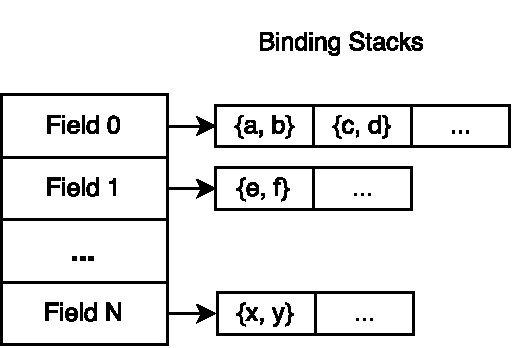
\includegraphics[scale=0.75,natwidth=203,natheight=298]{context}
\caption{The binding environment inside a context used to store the length and offset of fields, or the offset of headers. On the left, fields one through sixteen represent the fields that can be extracted. Each field maintains a binding list (stack). Each element in the binding list is a binding which stores the offset and length where each instance of that field can be found in the packet. }
\label{fg:ContextEnv}
\end{figure}

Figure \ref{fg:ContextEnvWorking} demonstrates how data is stored in the context as it is being decoded. The example is a packet which contains an encapsulated IPv4 header commonly used in IP tunneling. In the ethernet decoding stage which extract the \texttt{src}, \texttt{dst}, and \texttt{type} field are extracted and stored in the context. Next we determine that IPv4 follows based on the \texttt{type} field. We extract IPv4 \texttt{dst} and \texttt{protocol}. The \texttt{protocol} field tells us we have another IPv4 header after the current one. We move to decode that and once again we extract IPv4 \texttt{dst} and \texttt{protocol}. Note how the new values of IPv4 are pushed on top of the binding stack. Any further usage of those fields will use the latest values extracted for those fields. Keep in mind that this means any usage of the first set of IPv4 \texttt{dst} and \texttt{protocol} must occur before the decoding of the second IPv4 header.\

\begin{figure}
TODO: Make an image for this.
\caption{A context environment in action during runtime.}
\label{fg:ContextEnvWorking}
\end{figure}

The \textbf{action set} is the other major data structure contained within the context. The action set is a set of actions which have been written to the context for deferred execution using a \texttt{write action} (see Section \ref{action_tut}). Upon reaching a designated egress port, the action set is executed right before the packet is output.

\section{Table Stage} \label{table_desc}

Table stages handle matching against extracted fields, i.e. classification, and perform a sequence of desired actions on like-classified packets. This is done through a mechanism known as a flow table \cite{openflow_spec}.

A \textbf{flow table} is composed of a set of \textbf{flow entries}. A flow entry is composed of \textbf{match fields}, a \textbf{priority}, a set of \textbf{actions}, and miscellaneous additional data. Each table specifies a set of key fields that together make up a \textbf{key} for that table. For each key field, each flow entry has a corresponding value, known as a \textbf{match field}, such that every flow entry in the table is uniquely identified by its match fields and its \textbf{priority}.

When a packet reaches a table matching stage, the fields comprising the table's key are extracted from the context. Lookup into the table retrieves all flow entries whose match fields can correctly match the field values from the packet. The flow entry whose priority is highest is selected. The \textbf{actions} of the flow entry are executed on the packet.

If no such flow entry matches against the packet's field values, the \textbf{miss case} flow entry is applied to the packet instead. Flow entries can be user defined. By default, a miss in a table results in the packet being dropped. Miss cases always have the lowest possible priority amongst flow entries and each match field can be considered a wildcard.

The mechanic of table matching is not distinctly different from those of relational or SQL tables. In fact, Frenetic, another packet processing language, uses SQL-inspired syntax to classify flows \cite{frenetic_paper1}. If we make this comparison, a flow table is analogous to a SQL table, the concept of a key is the same for both, and a flow entry is analogous to a tuple in a SQL table. Each packet and its fields constitute the actual "query" into the table.

\section{Pipeline Composition} \label{pipeline_comp_desc}

Kinds of processing stages can be interleaved together in any order within the pipeline. This means that Steve is capable of supporting different packet processing paradigms found in other research such as POF and P4. With the Steve pipeline specification language a user can specify that a pipeline does:

\begin{enumerate}
\item \textbf{A full decode of the packet followed by a sequence of tables.} Packets coming to the pipeline have all necessary headers and fields are decoded and saved in the runtime context first. The packet is then dispatched to the first table in the pipeline. From there, matched flows within the tables dictate which table the packet is sent to next or which port the packet is forwarded to.
\item \textbf{A chain of partial decodes and table lookups.} Packets coming to the pipeline get partially decoded and dispatched to a table. The flow within that table could carry the packet to another table, another decoder, or forward it out of the network. The pipeline in this case in a chain of alternating sequences of decoding stages and table matching stages.
\item \textbf{Only decodes.} In some special cases, it may not even be necessary to go to a table matching stage. It may be possible to make a decision about the packet’s ultimate destination immediately upon evaluating a certain field within the packet using a simple conditional statement (if-statement, if-else statement, etc). Therefore, decoding stages also support the range of actions supported by flow entries, which can include outputting packets to a port or dropping it.
\end{enumerate}

Upon entering the pipeline, a packet must first go through at least one decoding stage before moving to the next processing stage. From there, the packet flows from one stage of the pipeline to the next. With each stage, certain conditions are evaluated which will determine where the packet must flow next. Finally, the packet will exit the pipeline either through a port(s) or by being dropped and discarded.

\chapter{The Steve Tutorial} \label{ch:tutorial}

\textit{How do I write a Steve program?} This chapter will answer this question through examples. Steve's primary focus is to provide language features for defining and connecting the pipeline processing stages described in Chapter \ref{ch:pipeline_model}. This chapter will explain how we write each of these components. Specifically, we will talk about how headers are represented, how to write decoders, how to write tables, and how to apply actions to packets.

By the end of this chapter, a user should be able to write many basic network applications using Steve. Three such applications will be presented: a simple learning switch, a simple learning router and a wire. Many of the examples presented throughout this chapter are just smaller parts of these applications presented in isolation. As we work through this tutorial, we will slowly build up these little components and explain what they do before finally presenting the complete program at the end.  

However, if you are feeling impatient, you may skip directly to these examples in Section \ref{tut:examples}.

As we walk through this tutorial, we will mention some semantics and limitations of Steve, but only in minor detail. For the complete semantic description of Steve, including grammar, typing rules, and other restrictions, see the User's Guide in Chapter \ref{ch:users_guide}. For a complete reference of all Steve grammar, see Appendix \ref{ap:a}.

\section{General Purpose Language Features} \label{tut:gen_purp}

Before we delve into language features specifically designed for packet processing, first we must mention a few language features which are more "general purpose." These language features are common to most programming languages and are not explicitly for packet processing, though they may prove useful. These language features are provided as part of the Beaker programming language \footnote{https://github.com/asutton/beaker} from which Steve derives.

\subsection{Variables} \label{tut:variable}

Steve allows us to allocate variables for storing values like any other language. Suppose we wanted to write a variable named \texttt{x} which holds an integer value \texttt{10}. We would write it as follows.

\begin{codepage}
\begin{lstlisting}
var x : int = 10;
\end{lstlisting}
\end{codepage}

Note that the type of the variable, \texttt{int}, follows the colon (\texttt{:}). We can assign a new value to it.

\begin{codepage}
\begin{lstlisting}
x = 1;
\end{lstlisting}
\end{codepage}

We can perform arithmetic and bitwise operations as well. The complete set of arithmetic and bitwise operations can be found in Section \ref{guide:binary_expr}.

\begin{codepage}
\begin{lstlisting}
var y : int = 2;
var z : int = 3;
y = x + y; // Adding
z = y + z + 1; 
z = z << 4; // Left shift.
var a : int = y & z; // bitwise and
\end{lstlisting}
\end{codepage}


\subsection{Conditional Statements} \label{tut:condition}

Steve supports some common language constructs for conditional decision making. Specifically, we have three conditional statements: the if statement, the if-else statement, and the match statement.

The if and if-else statements are written just like in most C-like languages. The behavior works the same as well.

\begin{codepage}
\begin{lstlisting}
var a : bool = true;
var b : bool = false;

// If statement
if (a || b) { }

// If else statement
if (a && b) { }
else if (a) { }
else { }
\end{lstlisting}
\end{codepage}

A match statement allows for a decision to be made given a number of possible case values. This makes it similar to a C-like switch statement, with the only major difference being that there is no "fall-through" behavior. In other words, after the execution of a case statement, control jumps out of the match statement rather than moving to the next case (i.e. an implied break). The condition and labels must be integers just like in C. A match statements can be written as follows.

\begin{codepage}
\begin{lstlisting}
// Assuming there are integer variables named x and y.
match (x) {
  case 0: x = x + 1;
  // Multiple statements following the label must be 
  // enclosed in a block.
  case 1: {
    x = x + 2;
    y = y * x;
  }
  
  // The default case statement.
  miss: x = 0;
}
\end{lstlisting}
\end{codepage}

Here, if \texttt{x} equals \texttt{0}, then \texttt{x = x + 1} gets executed. If \texttt{x} equals \texttt{1}, then two statements get executed in order: \texttt{x = x + 2}, then \texttt{y = y * x}. If \texttt{x} is neither, then \texttt{x = 0} is executed.

\subsection{While Loops} \label{tut:while}

While loops appear in Steve just like they appear in C-like languages. They also support the \texttt{break} and \texttt{continue} statements for limited branching abilities inside a loop.

In the following, we present a trivial while loop which demonstrates the basics of \texttt{break} and \texttt{continue}.

\begin{codepage}
\begin{lstlisting}
var x : int = 0;
var z : int = 0;
// Loop while x is less than 5.
while (x < 5) {
  x = x + 1;
  // If x equals 3, control goes back to the
  // first statement in the loop body.
  if (x == 3)
    continue;
    
  // This part is never reached if x == 2.
  // If z equals 2, then we exit the loop
  // altogether.
  if (z == 2) 
    break;
  // This will never execute when z == 2.
  z = z + 1;
}
\end{lstlisting}
\end{codepage}

Here, the value of \texttt{x} will be \texttt{4} and \texttt{z} will be \texttt{2} by the end of this loop.

The usage of while loops in packet processing right now is rather limited. Usage of loops will rarely come up in defining pipeline processing stages. However, they may become more useful as other features are added.

\subsection{Functions} \label{tut:function}

Steve supports writing simple functions, though the syntax is a little different from C-like languages. Functions can be called with parameters and can return results just like any other language. 

Suppose we wanted to write a function named \texttt{sum} which takes two integers, \texttt{a} and \texttt{b}, and returned the integer sum of \texttt{a} and \texttt{b}. We would write \texttt{sum} as follows.

\begin{codepage}
\begin{lstlisting}
def sum(a : int, b : int) -> int
{
  return a + b;
}
\end{lstlisting}
\end{codepage}

Note that the return type follows the \texttt{->} in Steve functions. To call the \texttt{sum} function we would write the following. Here, the result of \texttt{sum} would be \texttt{3}.

\begin{codepage}
\begin{lstlisting}
var x : int = 1;
var y : int = 2;
var z : int = sum(x, y);
\end{lstlisting}
\end{codepage}

\subsection{Literals} \label{tut:literal}

Steve supports decimal, binary, and hexadecimal integer literals. Steve does not currently support things like IP address literals or MAC address literals. Decimal integers can be written like any other language.

Binary literals all start with the prefix \texttt{0b} followed by any number of \texttt{0}'s and \texttt{1}'s. The underscore (\texttt{\_}) can optionally occur anywhere in the literal following the prefix; a feature similar to Java. This is purely for organization and readability.

\begin{codepage}
\begin{lstlisting}
// These are the same value.
0b10101010
0b1010_1010
\end{lstlisting}
\end{codepage}

Hexadecimal literals all start with the prefix \texttt{0x} followed by any number of digits between \texttt{0} and \texttt{9}. The underscore (\texttt{\_}) can optionally occur anywhere in the literal following the prefix similar to binary literals.

\begin{codepage}
\begin{lstlisting}
// These are the same value.
0x0800
0x08_00
\end{lstlisting}
\end{codepage}

\section{Layouts} \label{tut:layout}

Now that we've gotten the general purpose things out of the way, we can move on to packet processing specific language features.

\textit{Layouts} are something which will appear in almost all Steve programs. They let us describe the \textit{structure} of a packet header. More specifically, they describe \textit{what} fields are present, their \textit{lengths}, the \textit{order} in which they appear, and their \textit{relative offset} from the beginning of the header. Layouts become pivotal during decoding stages, where all this information is used to guide the extraction of fields from a packet. 

\textit{What is the difference between a layout and a header?} Before moving on, it is important to make this distinction clear. A layout is like a blueprint for a header. It gives us information; it \textit{describes} that header. The header is an actual sequence of bits, a portion of the packet, which we get off of the network. The header \textit{exists} whereas a layout merely helps us \textit{understands} it. 

\textit{How does one write a layout?} Let us begin with a simple example: the ethernet header \cite{eth_std}. Ethernet is a Layer 2 \cite{osi_model} protocol and the most common in use. The first header most programs decode will be ethernet.

An ethernet header has three fields: destination and source MAC addresses which are both 6 bytes (or 48-bits) long, and a type field which is 2 bytes (or 16-bits long). To write a layout describing the ethernet header, we use a \textit{layout declaration} (\ref{guide:layout}). In the following, we present an ethernet layout declaration matching these specifications.

\begin{codepage}
\begin{lstlisting}
// This layout describes the ethernet header.
layout ethernet
{
	// Each field is a pair of names and types.
	// Each type specifies that field's length.
	dst  : uint(48); // This is 48 bits long.
	src  : uint(48); // This is 48 bits long.
	type : uint(16); // This is 16 bits long.
}
\end{lstlisting}
\end{codepage}

Here, we declare a layout named \texttt{ethernet}. Each layout defines which fields it has with a \textit{field declarations} (\ref{guide:layout}). Each field is given a \textit{name} (\ref{guide:identifiers}) and a \textit{type} (\ref{guide:type}). In this example, we declare three such fields: \texttt{dst}, \texttt{src}, and \texttt{type}. The \textit{length} of each field is denoted by the \textit{size} required to store an object of that \textit{type}. Here, each field has unsigned integer type (\ref{guide:integer_type}), \texttt{uint}, with an (optional) precision. The precision denotes the size (in bits) needed to store that integer. Thus the \texttt{dst} and \texttt{src} fields have a length of 48 bits, and the \texttt{type} field has a length of 16 bits.

The \textit{relative offset} of each field is the number of bytes it is away from the beginning of the header. The first field will always have a relative offset of 0 bytes. The relative offset of each subsequent field is equal to the sum of the lengths of all fields preceding it. Here, \texttt{dst} has a relative offset of 0 bytes, \texttt{src} has one of 6 bytes, and \texttt{type} has one of 12 bytes.

Note that the fields appear in the order with which they would normally appear in an ethernet header. This is important. Field ordering should always be preserved when declaring layouts. If the ordering is incorrect, decoders will assume a sequence of bits is a certain field when it truly is not.

Not all header structures are as simple as the ethernet header. Sometimes we must deal with headers nested inside headers. It is for this very reason, that we allow layouts to be nested. 

In the following, we present such a case, where we expect a VLAN header \cite{vlan_std} is nested right before the \texttt{type} field of an ethernet header. 

\begin{codepage}
\begin{lstlisting}
// Layouts may be nested like this.
layout ethernet
{
  dst  : uint(48);
  src  : uint(48);
  vlan_tag : vlan; // Nested layout
  type : uint(16);
}

layout vlan
{
  type : uint(16);
  tci  : uint(16);
}
\end{lstlisting}
\end{codepage}

In this example, we declare two layouts: \texttt{ethernet} and \texttt{vlan}. To achieve a nested layout, we add a field named \texttt{vlan\_tag} to \texttt{ethernet}, and we give its type as the name of the layout, \texttt{vlan}. Then length of the \texttt{vlan\_tag} field would be the sum of its sub-fields, in this case, 32 bits.

\textit{How do layouts differ from classes in other languages?} With the way layouts are described, it is easy to draw the comparison between layouts and classes in object-oriented languages. However, layouts do \textbf{not} function like classes at all. Layouts are much stricter.

First of all, \textit{the types of each field are restricted}. Fields may only have two types: integer (\ref{guide:integer_type}) and layout (\ref{guide:layout_type}). There may be varying kinds of integer (e.g. precisions, signed, unsigned, etc.), but the precision of each integer must also be \textit{byte-aligned}, that is, a multiple of 8. 

Second, the most important distinction is that \textit{objects of layout type can never be created}. Layouts may not appear as the type of parameters, nor may they appear as return types. All of the following are considered illegal.

\begin{codepage}
\begin{lstlisting}
layout L1 { f1 : uint; f2 : uint(16); }
var x : L1 = 0; // Invalid.
// Invalid parameter type and return type.
def foo(y : L1) -> L1 { }
\end{lstlisting}
\end{codepage} 

Packets and their headers exist independent of a running Steve application. Layouts are purely used to guide decoding them. Additionally, there are a number of concerns related to constructing objects of layout type, thus such behavior is not allowed. For further details on layout limitations, refer to Section \ref{guide:layout} in the User's Guide.

Another important note is that Steve does not currently support dynamically sized types (DST). A DST is a type whose size is predicated upon some value known only during runtime. These DST's are used to represent fields whose lengths are dynamic. Some examples of dynamic length fields are the \texttt{options} fields in IPv4, IPv6, and TCP headers \cite{ipv4_std, ipv6_std, tcp_std}.

DST's are a language feature that will eventually be added, but are outside the current implementation. Because of this, fields whose lengths are dynamic cannot currently be declared, extracted, nor used. The existence and eventual support of DST's is one of the reasons why objects of layout type cannot be created. This is further discussed in Section \ref{guide:layout}.

In the following, we present a case where some of these limitations come into play -- the IPv4 layout. IPv4 is a Layer 3 protocol \cite{osi_model} and is used for routing. An IPv4 header appears in almost all Internet-bound packets and thus makes it a common layout to write. This layout will prove useful to us when defining the simple router program later on.

\begin{codepage}
\begin{lstlisting}
layout ipv4
{
  version_ihl : uint(8); // Non-byte aligned fields are merged.
  dscp_ecn    : uint(8);  // This is merged, too.
  len         : uint(16);
  id          : uint(16);
  fragment    : uint(16); // Fragment usually has flags.
  ttl         : uint(8);
  protocol    : uint(8);
  checksum    : uint(16);
  src         : uint(32);
  dst         : uint(32);
  // Note, the missing, unsupported options field.
}
\end{lstlisting}
\end{codepage}

In this example, we can seen that \texttt{version} (a 4 bit field) has to be merged with \texttt{ihl} (internet header length) (also a 4 bit field) to achieve byte alignment. The same is true for \texttt{dscp} and \texttt{ecn}. The \texttt{fragment} field, typically composed of three 1 bit flags and a 13 bit fragment offset field, is merged into a single 16 bit field. To recover the values of these sub-fields, we have to use logical-and (\ref{guide:bitwise_expr}) to mask the un-needed bits. An example will come up later when we discuss an IPv4 decoder.

\section{Decoders} \label{tut:decoder}

Decoding stages, or \textit{decoders} for short, are special purpose functions used to handle decoding and extracting fields from a \textit{single} header. By chaining multiple decoders together, a user can construct a sequence of functions used to parse an entire packet. 

When writing a decoder, it is good practice to keep the following in mind.

\begin{itemize}
\item Which header am I decoding? What layout will I use to guide the decoder?

\item What fields do I want from the header?

\item How will I use the extracted fields? Will I need to perform arithmetic or make decisions with them?

\item \textit{Actions} are used to manipulate packet fields, forward packets, and add/remove flow entries from tables. What actions do I want to take on the packet? Change a field value? Forward it? Drop it? 

\item What do I want to do next with the packet? Do I want to decode the next header? Do I want to send it to table matching? 
\end{itemize}

As we write these decoders, we too will answer these questions.

\subsection{The Basic Decoder Form} \label{tut:basic_decoder}

To write a decoder, we use a \textit{decoder declaration} (\ref{guide:decoder}). A decoder declaration has four important parts: 1) a name, 2) a \textit{layout rule}, 3) a keyword specifying whether this is the starting decoder, and 4) a body.

\textit{What is a layout rule?} A layout rule is the layout which the decoder will use to guide its extractions. It provides all the information necessary for the decoder to determine which bits in a packet comprise which fields. Here, we decide the answer to the questions, "Which header am I decoding? What layout will I use to guide the decoder?"

For our applications (and for almost all applications) we will need to decode ethernet first. We assume that all packets coming to our device begin with the ethernet header (the most common first header). Our decoder will look something like this:

\begin{codepage}
\begin{lstlisting}
// The empty ethernet decoder.
decoder start eth_d(ethernet) { }
\end{lstlisting}
\end{codepage}

In this example, our decoder is named \texttt{eth\_d}. The layout rule is \texttt{ethernet}. We also add the \texttt{start} keyword. This means this decoder will always be the first to execute. A program must have exactly one starting decoder. Our decoder has an empty body delimited by \texttt{\{\}}. As we go, we will fill in this body with instructions for the decoder.

\subsection{Extractions} \label{tut:decoder_extract}

The primary goal of a decoder is to extract fields from a single header. These extracted fields, or \textit{extractions} for short, are found using information gathered from the \textit{layout rule}.

To extract a field, we write an \textit{extract declaration} (\ref{guide:extract}) in the decoder's body. We decide that we want all fields extracted from the ethernet header. Our decoder now looks like the following.

\begin{codepage}
\begin{lstlisting}
// The ethernet decoder extracts all fields.
decoder start eth_d(ethernet) 
{
	extract ethernet.dst; 
	extract ethernet.src;
	extract ethernet.type; 
}
\end{lstlisting}
\end{codepage}

Each extract declaration gives a \textit{field name} (\ref{guide:field_name}). The field name refers to a field in the \textit{layout rule}. Here, \texttt{ethernet.dst}, \texttt{ethernet.src}, and \texttt{ethernet.type} are our field names.

We can only use field names which refer to fields in the layout rule. It would obviously make no sense to extract a field not in the header. The decoder gathers information to find the location and length of the field, then saves it in our context (\ref{context_desc}).

\subsection{How Decoder's Extract Fields} \label{tut:extract_how}

Before we continue, we must discuss exactly how a decoder uses a layout rule to extract fields. A decoder has a very limited look into a packet. It only has access to a subset of contiguous bytes, known as the \textit{view} of the decoder. A decoder's view begins where the header it decodes begins, and ends (implicitly) where that header ends. Its view ends implicitly because a layout only provides information on a single header's fields. It is obvious that a decoder would not be able to decode past the final field it knows about from its layout rule.

Figure \ref{fg:decoding} demonstrates how decoders and their views work. In this case, we are decoding a typical packet with ethernet, IPv4, and UDP headers. The starting decoder's view always starts at the beginning of the packet. In the case of Figure \ref{fg:view1}, the first header is ethernet.

\begin{figure}[ht]
\begin{subfigure}[t]{.45\textwidth}
  \centering
  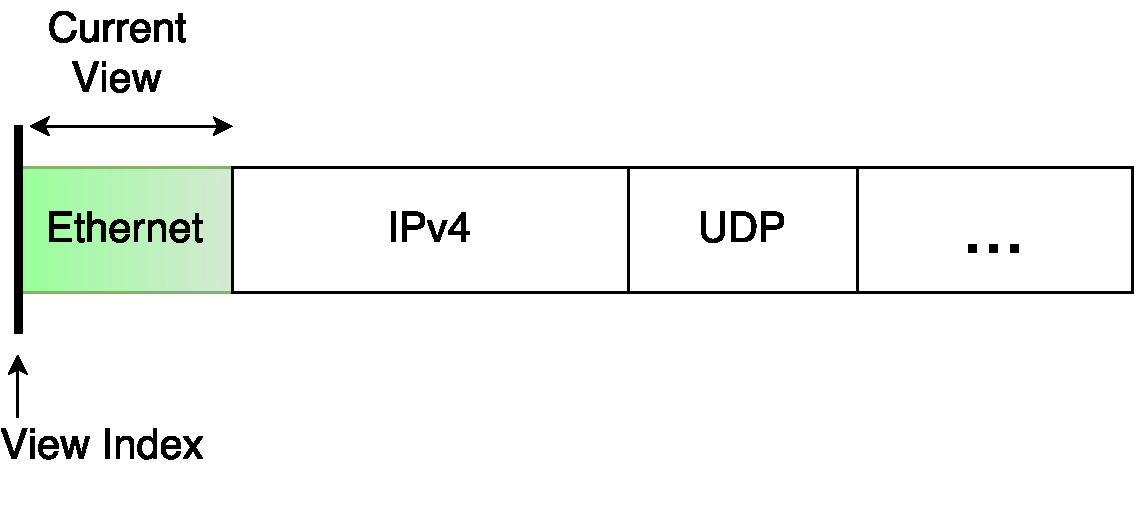
\includegraphics[width=.8\linewidth]{view1}
  \caption{We have the view of the starting decoder, in this case, the ethernet decoder. The beginning of the view is the same as the beginning of the ethernet header, which is also the beginning of the packet.}
  \label{fg:view1}
\end{subfigure}%
\hfill
\begin{subfigure}[t]{.45\textwidth}
  \centering
  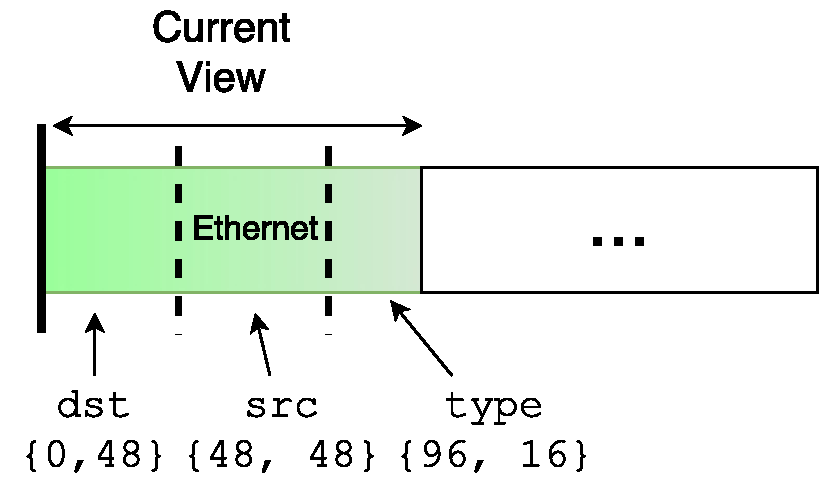
\includegraphics[width=.8\linewidth]{view2}
  \caption{The beginning of a field is discovered by its relative offset from the beginning of the view. The end is determined by the field's length. The field \texttt{dst} is 0 bytes from the beginning, \texttt{src} is 6 bytes in, and \texttt{type} is 12 bytes in.}
  \label{fg:view2}
\end{subfigure}

\begin{subfigure}[t]{.45\textwidth}
  \centering
  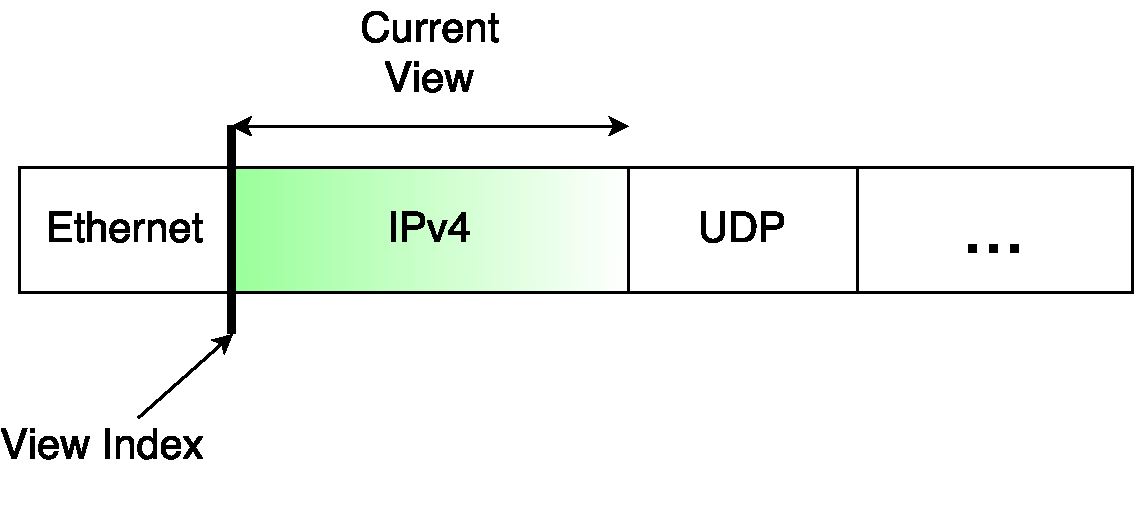
\includegraphics[width=.8\linewidth]{view3}
  \caption{When a decoder is finished working, it \textit{shifts} the view to the next header. The shift moves the beginning of the view by the length of the header -- 14 bytes.}
  \label{fg:view3}
\end{subfigure}%
\hfill
\begin{subfigure}[t]{.45\textwidth}
  \centering
  \includegraphics[width=.8\linewidth]{view4}
  \caption{The view shifts again by 20 bytes once the IPv4 decoder finishes.}
  \label{fg:view4}
\end{subfigure}
\caption{A demonstration of the decoding process in action.}
\label{fg:decoding}
\end{figure}

Each field in the header is discovered by information gathered by the layout rule. Recall that our layout rule tells us the location, or relative offset, of each field from the beginning of the header (which is equivalent to the beginning of the view). Also recall our layout rule gives us the length of each field. From here, our decoder can go about discovering which bits form each field as demonstrated in Figure \ref{fg:view2}.

When a decoder finishes, it \textit{shifts} the view, as seen in Figure \ref{fg:view3}. The beginning of the view is moved by the length of header. The view now starts one byte \textit{after} where the previous header ended. The end of the view is implicit. All decoders are responsible for shifting the view in preparation for the next decoder. Once the next decoder is reached, its view is already on the header it decodes. When this next decoder finishes, it shifts the view once again, as seen in Figure \ref{fg:view4}.

\subsection{Accessing Extracted Fields} \label{tut:decoder_access}

After extracting a field from a header, we generally want to use the \textit{value} of that extraction. To use the value of an extraction, we need the \textit{field access expression} (\ref{guide:field_access_expr}). When we use the field names from our extract declarations in other operations, such as the condition of an if-else statement, or an operand in addition, we use it to mean the value of that field. That field name \textit{becomes} a field access expression.

Now, let us go about using some of our extracted fields from the ethernet header. A typical operation on an ethernet header is determining which protocol it encapsulates, i.e. the header which comes next.

\begin{codepage}
\begin{lstlisting}
decoder start eth_d(ethernet) 
{
  extract ethernet.dst;
  extract ethernet.src;
  // Use the type field to determine info on the next header.
  extract ethernet.type;
  // Using a field access expression with logical operator >=
  if (ethernet.type >= 0x600) {
    // Then type determines what header comes next.
  }
  else if (ethernet.type <= 0x05dc) {
    // Then type is the length of the entire packet.
  }
  // ...
}
\end{lstlisting}
\end{codepage}

The IEEE ethernet standard says that \texttt{type} fields greater than or equal to \texttt{0x600} indicate the next header \cite{eth_std}. Any \texttt{type} fields less than \texttt{0x05dc} indicate the ethernet frame's length. Here, we use field access to compare \texttt{ethernet.type} to hexadecimal literals in an if-else statement to determine the meaning of that field.

Our field values can also be used in arithmetic operations, bitwise operations, and can be stored and assigned to local variables. In the following, we present a trivial IPv4 decoder demonstrating some of these basic operations.

\begin{codepage}
\begin{lstlisting}
decoder ipv4_d(ipv4)
{
  extract ipv4.len; // Note that we do not have to extract
  extract ipv4.version_ihl; // fields in order.
  extract ipv4.ttl;
  extract ipv4.src;
  extract ipv4.dst;
  
  // Drop dead packets.
  if (ipv4.ttl == 0) drop;
  
  // We can assign field values to variables
  var pktlen : uint = ipv4.len;
  // We can perform bitwise operations.
  var ihl : uint(8) = ipv4.version_ihl & 0x0f;
  // We can also perform shifts.
  var version : uint(8) = ipv4.version_ihl >> 4;
  
  // Determine what the Time-to-Live is after this
  // device finishes with the packet.
  var next_ttl : uint = ipv4.ttl - 1;
  // ...
}
\end{lstlisting}
\end{codepage}

In this example, we also present a solution for recovering non-byte aligned fields. We bitwise-and (\ref{guide:bitwise_expr}) \texttt{ipv4.version\_ihl} with \texttt{0x0f} to recover the \texttt{ihl} field. We left-shift \texttt{ipv4.version\_ihl} by 4 bits to get the \texttt{version} field. We also demonstrate subtraction on \texttt{ipv4.ttl}, another common operation when dealing with IPv4 headers.

Field access expressions do have a number of limitations. The following example demonstrates some of them.

\begin{codepage}
\begin{lstlisting}
decoder start eth_d(ethernet)
{
  // Error: Cannot use eth.type before its extracted.
  if (ethernet.type >= 0x600) { }
  
  extract eth.type;
  
  // Now that its been extracted ...
  // Error: Cannot assign to a field this way.
  ethernet.type = 0x800;
  // ...
}

decoder ipv4_decode(ipv4)
{
  // Error: eth.type was not extracted by this decoder.
  if (ethernet.type == 0x800) { }
  // ...
}
\end{lstlisting}
\end{codepage}

A field access expression can only be used \textit{after} an extract declaration is made for that field. After all, it is impossible to recover the value of a field which has not been extracted. By extensions, they cannot be used in decoders which have not extracted that field. A decoder focuses on exactly one header and has no knowledge of previous headers or extractions. 

Field access expressions cannot be assigned to like a variable. To modify the value of a field, a set action must be used (see Section \ref{tut:set_action} for an example).

\subsection{Moving to Other Stages} \label{tut:decoder_next}

Now that we have completed extracting fields, we must answer the question, "What do I do next?" Recall from Chapter \ref{ch:pipeline_model} that decoding and table matching stages can be chained together in a number of flexible ways. 

A decoder can move a packet to another decoder, table, or it can forward/drop the packet. It is up to the programmer to decide which is appropriate.

To move to another decoding stage, a decode action (\ref{guide:decode_action})) is used. In the following example, we bridge the ethernet and IPv4 decoders we declared in an earlier example. We use the match statement (\ref{guide:condition_stmt}) to check if \texttt{ethernet.type} is equal to \texttt{0x800}. If it is, we decide to use the decode action to move the packet to the IPv4 decoder.

\begin{codepage}
\begin{lstlisting}
decoder start eth_d(ethernet)
{
	extract ethernet.dst;
	extract ethernet.src;
	extract ethernet.type;
	if (ethernet.type >= 0x600)
	  	// The next header is IPv4 if the type field is 0x800.
	    match (ethernet.type) {
	      case 0x800: decode ipv4_d;
	    }
	// Do nothing.
}

decoder ipv4_d(ipv4) {
	// ...
}
\end{lstlisting}
\end{codepage}

To transition to a table matching stage, a goto action (\ref{guide:goto}) (not to be confused with a C-like \texttt{goto}) is used. 

\begin{codepage}
\begin{lstlisting}
decoder ipv4_d(ipv4)
{
  extract ipv4.version_ihl;
  extract ipv4.protocol;
  extract ipv4.src;
  extract ipv4.dst;
  // Calculate internet header length (ihl).
  var ihl : uint(8) = (ipv4.version_ihl & 0x0f) * 4;
  // We apply the advance clause to shift our view by a given
  // number of bytes.
  goto t1 advance ihl;
}
\end{lstlisting}
\end{codepage}

In this example, we use a goto action to send the packet to a hypothetical table named \texttt{t1}. We will go into more details about writing tables in the next section. The most important thing to note from this example is the \texttt{advance} clause.

Recall from Section \ref{tut:extract_how} that a decoder shifts the \textit{view} of a packet before moving to the next stage. That shift is by the length of the header. IPv4 headers are dynamic in length. Even though we do not currently support extracting dynamic length fields, we must still account for them. To correctly do this, we apply the \texttt{advance} clause which explicitly shifts the view by the given number of \textit{bytes}. The \texttt{advance} clause may appear on both goto and decode actions. 

The assumption is made that all headers are word-aligned, therefore advancing by a number of bytes (rather than bits) is appropriate. Also note that an \texttt{advance} clause may only appear in a decoder, as decoders are the only stage concerned with views.

A stage is \textit{complete} once it executes a decode or goto action, or finishes executing without a decode or goto. No actions written in that stage \textit{after} a decode or goto gets executed. These two actions are similar in semantics to a return within a function. If no stage transition happens at all, the packet exits the pipeline, as described in Section \ref{tut:pipeline_exit}.

\section{Tables} \label{tut:table}

The next stage to explore is the table matching stage. Each table matching stage handles exactly one \textit{flow table}. 

\textit{What does a flow table do?} A flow table classifies packets into groups based on values found in a subset of that packet's fields. In fact, it is a decision table, like those found in AI and heuristics based applications. 

\subsection{The Basic Table} \label{tut:basic_table}

Each flow table is comprised of three parts: 1) a name, 2) a \textit{key}, and 3) a set of \textit{flow entries}. Additionally, there may be three kinds of flow tables: \textit{exact}, \textit{prefix}, and \textit{wildcard}. Steve currently \textit{only} supports the exact flow table. With an exact match table, each field in the packet must \textbf{exactly} match a flow entry's \textit{match fields}. We will discuss what this means in a second.

First, in the following example, we present the basic form of a table named \texttt{ethtype}. A table's \textit{key} is the set of fields, known as \textit{key fields}, which that table uses for classifying packets. They are the equivalent of decision attributes. The \texttt{ethtype} table's key has a single field -- \texttt{ethernet.type}

\begin{codepage}
\begin{lstlisting}
// The ethtype exact match table. 
// This has a single key field: ethernet.type.
exact_table ethtype(ethernet.type) 
{
	// Flow entries... 
}
\end{lstlisting}
\end{codepage}

Next, we must define a set of \textit{flow entries}. Flow entries are like the rules of a decision table. If a packet's fields match certain values, a corresponding sequence of actions are performed. 

To write a flow entry, we use a \textit{flow entry declaration} (\ref{guide:tables}). A flow entry declaration has two parts: 1) \textit{match fields} and 2) an \textit{action sequence}. Match fields are values which correspond to the table's key fields. When a packet is matched against a table, the table compares the packet's fields with the match fields of each flow entry. A packet \textit{matches} a flow entry, if each field (which is part of the table's key) in the packet matches each match field in the flow entry.

An \textit{action sequence} is a sequence of operations which are applied in order if the packet matches a given flow entry. Section \ref{tut:action} describes how to use these actions, though we have already seen a few.

Recall that in our ethernet decoder, we decided to decode IPv4 by checking if the \texttt{ethernet.type} field was equal to \texttt{0x800} using a match statement. In fact, it could be said that we \textit{classified} packets based on that value and made a uniform decision on all packets that matched. 

Instead of making our decisions in conditional statements, we could also write a table which does the same thing. In the following example, we do just that.

\begin{codepage}
\begin{lstlisting}
// The ethtype exact match table. 
// This has a single key field: ethernet.type.
exact_table ethtype(ethernet.type) 
{
	// This flow entry matches all packets whose 
	// ethernet.type field equals 0x800.
	{ 0x800 } ->
	{
		// If it matches, send it to ipv4_d.
		decode ipv4_d;
	}
	// This is the miss case. It matches all packets
	// which do not match any other entry.
	miss ->
	{
		drop; // The drop action drops a packet.
	}
}
\end{lstlisting}
\end{codepage}

Here, we define two flow entries. The first flow entry is a typical one. Match fields appear as a comma-separated list of expressions in the brace-enclosed block before the \texttt{->}. Here, we have a single match field with a value of \texttt{0x800} corresponding to our single key field, \texttt{ethernet.type}. All packet's whose \texttt{ethernet.type} field is \texttt{0x800} will match this flow entry. Following the \texttt{->} within the brace-enclosed block is the action sequence. Here, we have a single action, the decode action, which will send the packet to the IPv4 decoder.

The second flow entry is known as the \textit{miss case}. The miss case flow entry gets matched if a packet matches no other flows. Here, we apply the drop action (\ref{guide:drop}) to drop any missed packets. By default, if no miss case is defined, an implicit miss case whose action sequence is a single drop action is added to the table.

Now if we re-write our ethernet decoder from before, we get essentially the same behavior.

\begin{codepage}
\begin{lstlisting}
decoder start eth_d(ethernet)
{
	extract ethernet.dst;
	extract ethernet.src;
	extract ethernet.type;
	goto ethtype;
}
\end{lstlisting}
\end{codepage}

Flow entries declared within a flow table, like in \texttt{ethtype}, are known as \textit{initial flow entries}. They get installed before a Steve application processes its first packet. Flow entries may also be added to a flow table. An example of adding flows can be found in Section \ref{tut:insert_flow_action}.

\subsection{A More Complex Table} \label{tut:complex_table}

So far we have only presented the most basic of flow tables. Flow tables can get far more complicated.

Not all flow tables will match on a single field. In fact, most flow tables will match on many fields. Some flow tables may even need fields extracted, yet not necessarily care what the values of those fields are. For example, an IPv4 table may want to decrement the time-to-live field. This is a common operation. Yet it does not care what the value of that field is (as long as it is greater than 0). For these cases, we have the \texttt{requires} clause.

The \texttt{requires} clause gives a sequence of fields which a table needs extracted before being reached, but whose value is irrelevant. Each \textit{required field} can be thought of as if it were a wildcard value (*).

In the following example, we present a table which matches on two fields, \texttt{ipv4.fragment} and \texttt{ipv4.protocol}, and requires \texttt{ipv4.ttl}.

\begin{codepage}
\begin{lstlisting}
// The key fields are ipv4.fragment and ipv4.protocol.
exact_table ip_proto(ipv4.fragment, ipv4.protocol)
	requires (ipv4.ttl)
{  
  // We have 0x0 for the fragment field
  // and 0x01 (ICMP) for the protocol field.
  // The fragment field is 0 when a packet isn't fragmented.
  { 0x0, 0x01 } ->
  {
  	set ipv4.ttl = ipv4.ttl - 1; // Decrement time-to-live.
  	// Dispatch to the ICMP Decoder.
  	decode icmp_d;
  }
  // And so on...
}
\end{lstlisting}
\end{codepage}

This flow table tries to classify packets to determine which transport layer protocol \cite{osi_model} they use, and dispatches to the appropriate decoder. Our flow entry restricts itself to only non-fragmented packets.

Recall from Section \ref{tut:decoder_access} that we could not assign directly to fields. Here, the set action (\ref{guide:set_field}) is used to assign a new value to the \texttt{ipv4.ttl} field.

Flow entries may also have \textit{properties}. Properties are additionally information stored alongside flow entries. Steve supports two properties: timeout and egress.

If the timeout property is set, the flow entry will be ejected from its table after a given number of seconds. This value may be between 1 and 65,535. The egress property stores a port and becomes useful later on for learning applications (see the learning switch example in Section \ref{tut:learning_switch}).

The following example extends the previous \texttt{ip\_proto} table.

\begin{codepage}
\begin{lstlisting}
// The key fields are ipv4.fragment and ipv4.protocol.
exact_table ip_proto(ipv4.fragment, ipv4.protocol)
	requires (ipv4.ttl)
{  
  // Previous flow entries...
  
  // The protocol field is 0x06 for TCP data.
  // The flow property-timeout-sets a timeout in secs.
  // A flow entry with a timeout is removed after X secs.
  [timeout = 1000]
  { 0x0, 0x06 } ->
  {
  	set ipv4.ttl = ipv4.ttl - 1; // Decrement time-to-live.
  	// Dispatch to the TCP Decoder.
  	decode tcp_d;
  } 
  // And so on...
}
\end{lstlisting}
\end{codepage}

This flow entry sets the timeout property in the \textit{properties block} preceding the usual flow entry declaration. The properties block is a comma-separated list of properties.

\subsection{The Reasoning Behind Flow Tables} \label{tut:why_tables}

\textit{What makes using a table different from decision structures like an if-else or match statements?} As anyone can tell, the \texttt{ethtype} table presented in Section \ref{tut:basic_table} could have been written as a simple match statement. What are the advantages?

\textit{Tables can match on one or more fields at once.} The more fields required in the decision making process, the more complex using nested decision structures gets. Tables can also match on a packet's ingress port (\texttt{in\_port}) and physical ingress port (\texttt{in\_phys\_port}) fields (described in Section \ref{tut:output_action}).

\textit{Tables can match on and use fields from different headers.} Unlike decoders, tables have access to all extractions. The only limitation is that field access only works on key fields or required fields. For example, the following is a valid table. 

\begin{lstlisting}
exact_table t1(in_port, in_phys_port, ethernet.dst, ipv4.dst) 
{
	// ... 
}
\end{lstlisting}

\textit{Flow entries can be added and removed from tables using the appropriate actions.} This allows decision making on packets to change dynamically during runtime. It is obviously impossible to add new branches to if-else and match statements. The ability to add, or \textbf{learn}, new entries allows us to write applications which can evolve, such as learning switches and routers. An example of adding flows can be found in Section \ref{tut:insert_flow_action}.

\section{Exiting the Pipeline} \label{tut:pipeline_exit}

\textit{When is pipeline processing complete?} A packet exits the pipeline when a stage finishes executing, and does not send the packet to another stage. For decoders, this means that its entire body has finished execution, but it has not used a decode or goto action. In the following example, if \texttt{ethernet.type} is not greater than or equal to \texttt{0x600}, pipeline processing completes. 

\begin{codepage}
\begin{lstlisting}
decoder start eth_d(ethernet)
{
	extract ethernet.type;
	if (ethernet.type >= 0x600) {
		// Do something...
	}
	// Do nothing. Packet exits pipeline.
}
\end{lstlisting}
\end{codepage}

If a drop action is applied like in the following example, pipeline processing immediately stops and the packet is dropped.

\begin{codepage}
\begin{lstlisting}
decoder ipv4_d(ipv4)
{
  extract ipv4.ttl;
  
  // Drop packets whose time-to-live expired.
  if (ipv4.ttl == 0) 
  	drop;
  // Nothing past here get's executed if ttl is 0...
}
\end{lstlisting}
\end{codepage}

For table stages, packets exit once a flow entry finishes executing its body and does not apply a goto or decode action.

\begin{codepage}
\begin{lstlisting}
exact_table t1(eth.type) {
	{ 0x880 } -> 
	{
		// This will write the output action to the action set.
		write output flood; 
		// Packet exits after the write action.
	}
}
\end{lstlisting}
\end{codepage}

Here, \texttt{t1}'s flow entry uses a write action (described in Section \ref{tut:write_action}) to write an output action to the packet's action set. Then, the packet exits the pipeline.

Once a packet completes pipeline processing, any actions written to its action set get executed. \textit{Written} output actions, when executed, modify the egress port field in the packet's context. This field ultimately decides where the packet gets forwarded once its action set is done executing. If nothing is written to this field, the packet is implicitly dropped.

\section{Ports} \label{tut:ports}

Ports are important, obviously, because packets are received from ports and forwarded through ports. Without them, there would be nothing to do with packets. The language supports two "kinds" of ports: \textit{reserved ports} and \textit{regular ports}.

\subsection {Reserved Ports} \label{tut:reserved_ports}

Reserved ports are ports which are always present on the system. Some ports may be directly forwarded to using the output action (demonstrated in Section \ref{tut:output_action}). Other reserved ports are forwarded to implicitly by other actions.

The following reserved ports may be forwarded to by the output action.

\begin{itemize}
\item Forwarding to the \textit{all} port will forward copies of the packet to every port on the system.

\item Forwarding to the \textit{reflow} port will send the packet back into ingress processing. From there it will be processed again by the pipeline from the beginning.

\item Forwarding to the \textit{flood} port sends copies of the packet to all ports on the system \textit{except} the packet's ingress port.
\end{itemize}

Each of these reserved ports can be accessed using a reserved keyword. In the following, we show the output action being used to send a packet to these three ports.

\begin{codepage}
\begin{lstlisting}
all; // The all port
reflow; // The reflow port
flood; // The flood port

// Output action with these ports.
output all;
output reflow;
output flood;
\end{lstlisting}
\end{codepage}

The following reserved ports will be forwarded to by other actions.

\begin{itemize}
\item Packets are forwarded to the \textit{drop} port by the drop action. Packets which are dropped get deleted.

\item Packets are forwarded to the \textit{controller} port when the raise action is used. On the controller port sits a thread or program which will execute event handlers (explained in Section \ref{tut:event}) on packet contexts. Forwarding to the controller port is reserved only for exceptional events.
\end{itemize}

\subsection{Regular Ports} \label{tut:regular_ports}

Regular ports are any ports on the system which are neither reserved nor are always present. These ports can be split into \textit{physical} and \textit{logical} ports. A physical port is a hardware interface on the system. A logical port is a switch defined port which may map to multiple physical ports and include additional abstractions.

Steve applications currently do not support a way of directly discovering all these ports and their capabilities. Steve applications can indirectly "learn" about these ports over time by observing in the ingress ports of packets passing through the pipeline.

To get the logical ingress port and physical ingress port of a packet we have a number of reserved keywords.

\begin{codepage}
\begin{lstlisting}
in_port; // The logical ingress port.
in_phys_port; // The physical ingress port.

// Output action with these ports.
output in_port; // Send the packet back where it came from.
output in_phys_port;
\end{lstlisting}
\end{codepage}

\subsection{Port Variables} \label{tut:declared_ports}

Port variables can be used to "remember" ports for later usage. They can be written using \textit{port declarations} (\ref{guide:port}) as follows.

\begin{codepage}
\begin{lstlisting}
Port p1; // Two port variables.
Port p2;
\end{lstlisting}
\end{codepage}

Other ports can be assigned to them. This does not copy the port. It just saves a handle to that port inside the port variable.

\begin{codepage}
\begin{lstlisting}
p1 = in_port; // "Remember" a logical ingress port of a packet
p2 = in_phys_port; // and a physical ingress port.

output p1; // Forward to these ports.
output p2;
\end{lstlisting}
\end{codepage}

Here, it is shown that the names of these port variables may also appear in output actions.

\section{Actions} \label{tut:action}

Actions change packets, action sets, and pipeline state. Steve supports ten actions with more anticipated in the future. Actions can be used in both decoders and flows in Steve.

\subsection{Decode Action} \label{tut:decode_action}

The \texttt{decode} action is used to move a packet from the current stage to a decoding stage. This action was present throughout a number of examples. As a reminder, assume we want to move to an IPv4 decoder named \texttt{ipv4\_d}, the action would be written as:

\begin{lstlisting}
decode ipv4_d;
\end{lstlisting}

Remember that there is also an optional \texttt{advance} clause which is used if the \textit{view} of the packet must be explicitly shifted by some special number of bytes. For example, if the current decoder is for IPv4, and the next decoder is named \texttt{udp\_d}, the action would be written as:

\begin{lstlisting}
decode udp_d advance (ipv4.version_ihl & 0x0f) * 4;
\end{lstlisting}

The \texttt{advance} clause may only be attached if the action is executed by a decoder. Only decoders are responsible for view shifts.

\subsection{Goto Action} \label{tut:goto_action}

The \texttt{goto} action is used to move a packet from the current stage to a table matching stage. Assume we want to move to a table named \texttt{t1}, the action would be written as:

\begin{lstlisting}
goto t1;
\end{lstlisting}

Similar to the \texttt{decode} action, the \texttt{goto} action also supports an optional advance clause. For example, if the current decoder is for IPv4, and the table is named \texttt{t1}, the action would be written as:

\begin{lstlisting}
goto t1 advance (ipv4.version_ihl & 0x0f) * 4;
\end{lstlisting}

The \texttt{advance} clause may only be attached if the action is executed by a decoder. Only decoders are responsible for view shifts.

\subsection{Insert Flow Action} \label{tut:insert_flow_action}

Inserting flow entries into a table is a Steve action not explicitly supported by the OpenFlow standard \cite{openflow_spec} though it is supported in software switches like OVS \cite{ovs_man_page}. 

Flow entries can be inserted with constant key values and no properties. Here, we insert a flow entry into the table presented in Section \ref{tut:complex_table}.

\begin{codepage}
\begin{lstlisting}
// Constant key values.
insert
{ 0x0, 0x89 } ->
{
  set ipv4.ttl = ipv4.ttl - 1;
  decode mpls_d;
} 
into ip_proto;
\end{lstlisting}
\end{codepage}

They can also be inserted with field values of the current packet and with optional properties.

\begin{codepage}
\begin{lstlisting}
// Dynamic key values
insert
[timeout = 1000, egress = in_port]
{ ipv4.fragment, ipv4.protocol } ->
{
  output egress;
} 
into ip_proto;
\end{lstlisting}
\end{codepage}

In this case, the flow entry uses the \texttt{ipv4.src} and \texttt{ipv4.dst} fields of current packet as values for the inserted flow entry's match fields. It also sets the timeout to 1000 and sets the \texttt{egress} property to the current packet's \texttt{in\_port}, making the \texttt{output egress} action valid.

If a new flow entry's match fields already exist in the table, the old flow entry is replaced by the new flow entry. A miss case may be inserted into a table as well.

\begin{codepage}
\begin{lstlisting}
insert 
miss -> { output flood; } 
into ip_proto;
\end{lstlisting}
\end{codepage}

\subsection{Remove Flow Action} \label{tut:remove_flow_action}

A flow entry can be removed from a table by providing match field values and the name of the table to remove the flow entry from. This can be done with constant values or dynamic field values of the current packet. If the flow entry with those match field values does not exist, nothing is done.

\begin{codepage}
\begin{lstlisting}
// Removal with constant values.
remove { 0x0, 0x01 } from ip_proto;

// Or dynamic values.
remove {ipv4.fragment, ipv4.protocol} from ip_proto;
\end{lstlisting}
\end{codepage}

Miss cases can also be removed from tables. When a miss case is removed, it is replaced by the default flow entry (which drops the packet).

\begin{codepage}
\begin{lstlisting}
// Removing a miss case.
remove miss from t1;
\end{lstlisting}
\end{codepage}

\subsection{Output Action} \label{tut:output_action}

Output actions forward a \textit{copy} of the current packet to a port. As mentioned earlier in Section \ref{tut:ports}, an output action may forward to a number of ports named by keywords (\texttt{all}, \texttt{flood}, \texttt{reflow}, \texttt{in\_port}, \texttt{in\_phys\_port}), or may be forwarded to a port saved by a port variable.

\begin{codepage}
\begin{lstlisting}
// Output to reserved ports.
output all; // The all port.
output reflow; // The reflow port.
output flood; // The flood port.

// Output to physical & logical ingress ports.
output in_port;
output in_phys_port;

// Output to port variables.
output p1; // Assuming there is is a port variable named 'p1'.
\end{lstlisting}
\end{codepage}

Note that when an output action is immediately applied, a \textit{copy} of the packet is always forwarded. This means multiple output actions can be written in the same table or decoder. It also means that pipeline processing will continue on the original packet.

The \textit{original} packet is forwarded once pipeline processing completes. The destination port of the original packet is determined by a written output action (described in Section \ref{tut:write_action}).

If a flow has its egress port property set, it is possible to output to that port. In the following, a flow is inserted with its egress property set to the current packet's ingress port. Within the flow body, the output action forwards to the port saved by the egress port property.

\begin{codepage}
\begin{lstlisting}
// An inserted flow entry has its egress property set.
insert
[egress = in_port]
{ 0xffffffffffff } ->
{
	// We can output to egress.
	// This will forward all matching packets to the 
	// current packet's ingress port.
	output egress;
} 
into t1;
\end{lstlisting}
\end{codepage}

\subsection{Drop Action} \label{tut:drop_action}

A packet can be dropped by the Steve application using the \texttt{drop} action. The drop action immediately ends the pipeline processing of a packet.

\begin{codepage}
\begin{lstlisting}
drop;
\end{lstlisting}
\end{codepage}

\subsection{Set Action} \label{tut:set_action}

A \texttt{set} action can be used to write to any extracted field within a packet. For example, the time-to-live field from an IPv4 header may be set as follows.

\begin{codepage}
\begin{lstlisting}
set ipv4.ttl = ipv4.ttl - 1;
\end{lstlisting}
\end{codepage}

The \texttt{set} action is only valid if the field access expression is valid in that stage. For decoders, this means the field has to have been extracted first. For tables, this means the field must be a key field or a required field. For events, the field must be a required field.

\subsection{Write Action} \label{tut:write_action}

The context data structure described in Section \ref{context_desc} keeps an \textit{action set}. Actions get written to the action set using the \texttt{write} action. Written actions get executed once pipeline processing completes.

Only two actions may be written to a packet right now: output and set.

\begin{lstlisting}
// Writing a set action
write set ipv4.ttl = ipv4.ttl - 1;
// Writing an output action.
write output reflow;
\end{lstlisting}

The written output action has a slightly different semantic from the immediately applied output action. When immediately applied, the output action forwards a \textit{copy} of the packet. The write output action sets the egress port field in the packet context. This field ultimately decides where to forward the \textit{original} packet.

\subsection{Clear Action} \label{tut:clear_action}

The clear action removes all actions from the context's action set.

\begin{lstlisting}
clear;
\end{lstlisting}

\subsection{Raise Action} \label{tut:raise_action}

A \texttt{raise} action is used to trigger an \textit{event}. Events are used to handle exceptional situations described in Section \ref{tut:event}. Events define \textit{event handlers} which operate on a packet context. A raise action sends a copy of the packet context and the event handler to the controller port. On the controller port sits a thread or program (implementation specific) which executes these event handlers. A raise action is written as follows.

\begin{lstlisting}
// Assuming we have an event named "learn_event"
raise learn_event;
\end{lstlisting}

\section{Events} \label{tut:event}

An \textit{event stage} is a special processing stage outside the regular run-to-completion pipeline. Event stages are used to deal with exceptional situations. Event stages define \textit{event handlers} which are special functions that operate on packet contexts. Event handlers do not execute and block until completion. Blocking can severely bottleneck performance.

Specifically, inserting and removing flow entries are best executed inside events. These operations are extremely expensive. They are atomic and require locking tables in multi-threaded architectures.

An event is \textit{raised} using the raise action explained in Section \ref{tut:raise_action}. When an event is raised, the packet context and event handler are forwarded to the reserved controller port. On the controller port awaits a thread or program which will execute these event handlers as they are received.

To write an event handler, we use an \textit{event declaration} (\ref{guide:event}). Event declarations have a \texttt{requires} clause, just like tables. An event may only be raised if all fields listed in its \texttt{requires} clause have been extracted.

In the following example, we present a simple, nonsense event declaration. Here, our event requires the \texttt{ethernet.src} and \texttt{ethernet.type} fields be extracted. Inside the event, we can write any statements (such as if, match, assignment, variable declarations, etc.) and any actions described in Section \ref{tut:action}.

\begin{codepage}
\begin{lstlisting}
// A dummy event.
event e1
	requires(ethernet.src, ethernet.type)
{
	if (ethernet.type == 0x800) {
		// Do something...
	}
	else if (ethernet.src > 0x00_12_34_56_78_9a) { }
	var x : uint(48) = 0;
	set ethernet.src = x;
	output reflow;
	// Perform some other actions...
}
\end{lstlisting}
\end{codepage}

An important thing to know is that a \textit{copy} of the context is operated on by an event handler. Any changes made in the event handler does not modify the original packet or its context. An event handler may be executed immediately after a raise action is used, or it may be executed asynchronously. The decision is Flowpath (\ref{ch:flowpath}) implementation specific and the user should not rely on one or the other being the case.

Note that this feature is actually completely contrary to OpenFlow semantics \cite{openflow_spec}. Typically, a completely independent program defines event handlers and that program waits on the controller port for packets to process. Here, we allow those functions to be defined in Steve.

The advantage here is that Steve events are written as part of the Steve application and are thus subject to the same semantic, logical, and safety guarantees applied to other pipeline stages. 

\section{Examples} \label{tut:examples}

As promised at the beginning of this tutorial, we would demonstrate how to write three basic network applications: a learning switch, a learning router, and a wire using language features taught during this tutorial.

\subsection{The Learning Switch} \label{tut:learning_switch}

Let us begin by writing the Layer 2 (ethernet) learning switch. The learning switch shall receive packets. The ethernet header keeps track of the source and destination MAC addresses of a packet. Pipeline stages always know which port a packet enters the switch on. Learning applications exploit the likelihood that a path towards a networking device with that source MAC address exists through that port. This prevents the need to constantly flood packets on all ports.

With each packet, the switch will "learn" which MAC addresses are likely found on which ports by checking the source address. The switch forwards packets by looking at the destination address and checking if it has learned that MAC address yet. If it has not learned the address, it floods the packet.

The first step in writing any Steve application is defining the layouts. A learning switch only concerns itself with the ethernet header. We will use the ethernet layout we defined earlier.

\begin{codepage}
\begin{lstlisting}
// This layout describes the ethernet header.
layout ethernet
{
	dst  : uint(48); // This is 48 bits long.
	src  : uint(48); // This is 48 bits long.
	type : uint(16); // This is 16 bits long.
}
\end{lstlisting}
\end{codepage}

Our next step is the ethernet decoder. Since we are only concerned with the ethernet header, there is no reason to concern ourselves with \texttt{ethernet.type}.

\begin{codepage}
\begin{lstlisting}
decoder start eth_d(ethernet)
{
	// Extract the src and dst MAC addresses; type isn't needed.
	extract ethernet.dst; 
	extract ethernet.src;
	goto learn; // We proceed to the first table stage.
}
\end{lstlisting}
\end{codepage}

From here, we will need two tables: a learning table and a forwarding table. Using two tables will be typical of almost all learning applications. Both our tables will start out with nothing but a miss case. After all, before an application runs, it has not learned anything yet. The first few packets will certainly match against these miss cases.

The learning table is responsible for learning MAC addresses. This table will cause new flow entries to be inserted into both of our tables. The learning table matches on \texttt{ethernet.src}. A flow entry will be installed into this table to prevent the same \texttt{ethernet.src} from being learned multiple times. 

\begin{codepage}
\begin{lstlisting}
// This packet will cause new addresses to be learned.
exact_table learn(ethernet.src)
{
  miss ->
  {
  	// We raise an event to learn the appropriate flow entries.
  	raise learn_mac;
    goto forward; // Then send to the forwarding table.
  }
}
\end{lstlisting}
\end{codepage}

To insert the necessary flow entries, the \texttt{learn} table raises an event called \texttt{learn\_mac}. We will explore how this event is written shortly. After this event is raised, the learning table sends the packet to the forwarding table.

The forwarding table contains flow entries which will ultimately decide where to forward a packet based on its destination MAC address. The forwarding table thus matches on \texttt{ethernet.dst}. If the table has yet to determine which port that destination is likely found on, it floods the packet to all ports.

\begin{codepage}
\begin{lstlisting}
// This table ultimately decides which packet to forward on.
exact_table forward(ethernet.dst)
{
  // Flood any packet which hasn't been learned yet.
  miss -> { output flood; }
}
\end{lstlisting}
\end{codepage}

Now we revisit the \texttt{learn\_mac} event. This event is where the actual "learning" happens, and is thus the most important snippet of code in this application. The one extraction our event will need is \texttt{ethernet.src}. This is the MAC address the tables will be learning.

\begin{codepage}
\begin{lstlisting}
// This event will do the "learning" through flow inserts.
event learn_mac
	requires(ethernet.src) // It requires the src MAC
{
	// First we insert the src of the packet
	// into the learn table so we don't keep
	// trying to learn something we already have.
	insert
	[timeout = 60]
	{ ethernet.src } -> { goto forward; }
	into learn;
	
	// Next we insert the src of the current packet 
	// into the forward table.
	//
	// The forward table matches on the dst field of a packet. 
	// What we are doing is saying any packet whose dst is equal
	// to this packet's src is forwarded to this packet's
	// ingress port.
	insert
	[timeout = 60, egress = in_port]
	{ ethernet.src } ->
	{
		// We set the egress property to the current
		// packet's in_port. Future packets will be forwarded to
		// the current packet's ingress port.
		output egress;
	}
	into forward;
}
\end{lstlisting}
\end{codepage}

Our event will insert two flow entries. The first flow entry is inserted into the learning table. This entry prevents the same MAC address from raising the \texttt{learn\_mac} event more than once. Instead, the new flow entry sends the packet directly to the forwarding table.

The second flow entry is where our application actually "learns" the new MAC address. It is here where we establish set of MAC address to port mappings.

Recall that \texttt{forward} matches on \texttt{ethernet.dst}. Here, we insert a flow entry with the \textit{current} packet's \texttt{ethernet.src} value into \texttt{forward}. This means that all \textit{future} packets whose \texttt{ethernet.dst} equals the \textit{current} packet's \texttt{ethernet.src} will match our inserted flow entry. We also set the egress property equal to the \textit{current} packet's ingress port. Our flow entry's body subsequently uses \texttt{output egress}. Here, our MAC address to port mapping is complete.

To summarize, the second flow entry ensures that all future packets whose \texttt{ethernet.dst} field match the current packet's \texttt{ethernet.src} field will be forwarded to the current packet's ingress port.

\subsection{The Learning Router} \label{tut:learning_router}

The learning router is not too different from the learning switch. Instead of learning and forwarding from MAC addresses, this application will use IPv4 addresses.

We start again by defining our needed layouts. We may reuse the ethernet layout from the learning switch found in Section \ref{tut:learning_switch}. In addition, we will need an IPv4 layout.

\begin{codepage}
\begin{lstlisting}
// The layout needed to decode ipv4 headers.
layout ipv4
{
  version_ihl : uint(8);
  dscp_ecn    : uint(8); 
  len         : uint(16);
  id          : uint(16);
  fragment    : uint(16);
  ttl         : uint(8);
  protocol    : uint(8);
  checksum    : uint(16);
  src         : uint(32);
  dst         : uint(32);
}
\end{lstlisting}
\end{codepage}

Next, we will need the ethernet decoder. This time, we do not care about MAC addresses. Instead, we need to check the \texttt{ethernet.type} field to confirm this is an IPv4 packet. If it is, we send the packet to the IPv4 decoder.

\begin{codepage}
\begin{lstlisting}
decoder start eth_d(ethernet)
{
	extract ethernet.type;
	if (ethernet.type >= 0x600)
	  	// The next header is IPv4 if the type field is 0x800.
	    match (ethernet.type) {
	      case 0x800: decode ipv4_d;
	    }
	// If its not IPv4, processing ends and the packet is
	// implicitly dropped.
}
\end{lstlisting}
\end{codepage}

The IPv4 decoder will need to extract \texttt{ipv4.src} and \texttt{ipv4.dst} in order to learn them. Additionally, we'll need \texttt{ipv4.version\_ihl} to correctly advance past the IPv4 header and \texttt{ipv4.ttl} to decrement.

\begin{codepage}
\begin{lstlisting}
decoder ipv4_d(ipv4)
{
	extract ipv4.version_ihl; // Needed for ihl.
	extract ipv4.src; // Extract the IP addresses.
	extract ipv4.dst;
	extract ipv4.ttl; // We need ttl to decrement.
  
	// Drop on expired packets.
	if (ipv4.ttl == 0) drop;
	// Proceed to the learn table after advancing by ihl
	goto learn advance (ipv4.version_ihl & 0x0f) * 4;
}
\end{lstlisting}
\end{codepage}

We will need two tables just like in the learning switch example: learning and routing. Here, the \texttt{learn} table matches on \texttt{ipv4.src}. It will cause the IPv4 address to be learned. It will also prevent the same IPv4 address from being learned multiple times.

\begin{codepage}
\begin{lstlisting}
// The learn table will cause addresses to be learned.
exact_table learn(ipv4.src)
{
	miss ->
	{
		// It raises the event which will insert new flow entries.
		raise learn_ip;  
		goto routing;
	}
}
\end{lstlisting}
\end{codepage}

The routing table matches on \texttt{ipv4.dst}. This table will establish IPv4 address to port mappings. It will forward all packets whose destination IPv4 address it has learned. Any IPv4 addresses not yet learned are flooded by default.

\begin{codepage}
\begin{lstlisting}
// This ultimately decides where to forward packets based on
// their destination IP.
exact_table routing(ipv4.dst)
	requires(ipv4.ttl)
{
	miss -> 
	{ 
		set ipv4.ttl = ipv4.ttl - 1; // Decrement ttl
		output flood; // Flood on all unlearned addresses.
	} 
}
\end{lstlisting}
\end{codepage}

Lastly, we need to define the \texttt{learn\_ip} event which is, once again, largely the same as the \texttt{learn\_mac} event from the learning switch.

\begin{codepage}
\begin{lstlisting}
// This event handles the actual "learning."
event learn_ip
	requires(ipv4.src) // It will learn src IP addresses.
{
	// This first entry prevents the same address from causing
	// this event twice. It sends the packet straight to routing.
	insert
	[timeout = 30]
	{ ipv4.src } -> { goto routing; }
	into learn;
	
	// This establishes the IP address to port mapping.
	// Any packet whose dst address matches the current packet's
	// src address will be forwarded to the current packet's
	// ingress port.
	insert
	[timeout = 30, egress = in_port]
	{ ipv4.src } -> 
	{ 
		set ipv4.ttl = ipv4.ttl - 1; // Decrement ttl.
		output egress; 
	}
	into routing;
}
\end{lstlisting}
\end{codepage}

The first inserted flow entry prevents the same IPv4 address from being learned more than once. The second insert flow entry inserts the routing rule into the routing table. Any packet whose \texttt{ethernet.dst} is equal to the current packet's \texttt{ethernet.src} will be forwarded to the current packet's ingress port.

\subsection{The Wire} \label{tut:wire}

A wire is a network application which has two ports. It receives from one port and outputs out of the other port. The only caveat is that the application is not aware of the ports comprising the wire at first. It must learn that those ports exist.

This example demonstrates a number of more unintuitive features related to ports. First, we declare two uninitialized port variables named \texttt{p1} and \texttt{p2}. Uninitialized port variables always compare equal to 0.

\begin{codepage}
\begin{lstlisting}
// Our uninitialized port variables.
// These will compare equal to 0 at first
Port p1; .
Port p2;
\end{lstlisting}
\end{codepage}

Next, we'll use the ethernet layout from prior examples and write a decoder. The special thing about this decoder is that we do not care about any of the fields. We only need the ingress port.

\begin{codepage}
\begin{lstlisting}
decoder start eth_d(ethernet)
{
	// We use the port variables, p1 and p2, to "remember" ports.
	
	// Whenever a packet is handled, check if p1 and p2 are set.
	// If neither are, set p1 equal to the ingress port.
	if (p1 == 0 && p2 == 0)
		p1 = in_port;
	// If p1 is set, and p2 isn't, set p2 to the ingress port.
	else if (p1 != 0 && p2 == 0)
		p2 = in_port;
	
	// Now we decide which packet to forward to.
	// If the ingress port is p1, and p2 is set, forward to p2.
	if (in_port == p1 && p2 != 0)
		output p2;
	// If the ingress port is p2, and p1 is set, forward to p1.
	if (in_port == p2 && p1 != 0)
		output p1;
		
	// If both are not set yet, do nothing and implicitly drop.	
}
\end{lstlisting}
\end{codepage}

Here, we use the two port variables to "remember" what ports exist. The decoder looks at the ingress port and saves it into one of the two variables. Once two ports are "remembered," forwarding decisions can be made. If a packet comes from \texttt{p1}, then it is forwarded through the only other port, \texttt{p2}, and vice-versa. Before both ports are saved, since no other actions are applied, the packet finishes pipeline processing and gets dropped. 

\chapter{Freeflow and Steve Compilation} \label{ch:flowpath}

To load a Steve application, a switch must expose an application binary interface (ABI) which the Steve program can call to access switch resources and optimized operations. The desire is to push as much of processing logic into the hardware as possible 
so that the application does not have to know about the underlying switch architecture and optimize for it.

The Steve application also provides an interface so that the switch may use it to configure its pipeline, decode packets, and access event handlers.
The topic of this chapter will be describing these two interfaces.

To validate that this approach works, Steve targets a software data plane called Freeflow Virtual Machine (FFVM) \cite{freeflow_software}. FFVM is programmable and protocol independent. FFVM provides the runtime environment which exposes the ABI that Steve uses to manipulate the switch. FFVM virtualizes switch hardware as depicted in Figure \ref{fig:architecture}. Note that, though Steve targets FFVM, it could also directly target any software or hardware that exposed the same ABI.

%
%The Freeflow Virtual Machine (FFVM) is a software data plane that is programmable and protocol independent \cite{freeflow_software}. Freeflow provides a runtime environment (FFRT) for networking applications. FFRT is designed to abstract underlying hardware such as ports, memory, and flow tables. It exposes these resources through an interoperable ABI which can be used by almost any language. 
%
%Applications which target the FFVM ABI are called \emph{Freeflow managed applications}.
%These applications are dynamic link libraries (DLLs) designed to be loaded by FFVM.
%Their purpose is to program the data plane's packet processing pipeline by providing decoding logic and flow table configuration. They also act as the non-distributed controller for the Freeflow data plane. The architecture of this system is depicted in Figure \ref{fig:architecture}.

\begin{figure}[ht]
\centering
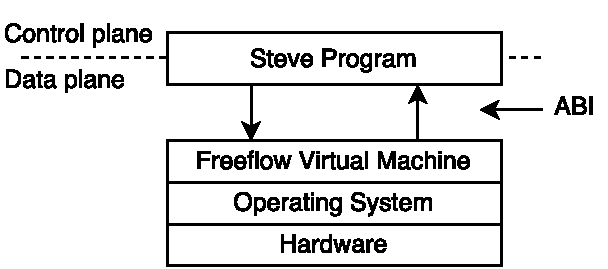
\includegraphics[scale=0.75]{architecture}
\caption{The FFVM architecture. FFVM virtualizes the underlying switch hardware and switch OS. Steve programs are loaded by FFVM and instantiates the data plane's pipeline. The Steve program also serves as the device's controller.}
\label{fig:architecture}
\end{figure}


%These other programs, known as \textit{pipeline applications}, contain all the packet processing logic. Packet decoders, flow table configuration details, flow entry definitions, and exceptional event handlers are contained inside these pipeline applications.
%Freeflow is designed to load these pipeline applications which are dynamic link libraries confirming to a certain Freeflow specification. Encapsulating all this functionality into these applications makes the data plane incredibly modular. The entire behavior of the data plane can instantly change by removing one application and loading another without having to stop and recompile the data plane's software. For example, in seconds, a Freeflow data plane instance can go from being an L2 switch to and L3 switch just by changing applications. 

%For now, the Steve compiler is specifically tailored toward compiling Freeflow pipeline applications. This chapter will focus on Freeflow, its interactions with Steve, and how Steve applications use the Freeflow API in its packet processing pipeline. 

\section{Freeflow ABI} \label{fp:dp_interface}

The Freeflow Runtime Library is the current ABI which Steve targets. It exposes a set of \emph{system calls} through functions which allow applications to gain controlled access to switch resources. Table \ref{tbl:Freeflow_api} summarizes the common usage of the library.

The runtime library provides four major facilities that the Steve application takes advantage of. The first is the ability to create tables with certain specifications. The second is the ability to add and remove entries from tables to manipulate forwarding logic. The third is the ability to queue up contexts that raised events and the event handlers that will deal with them. The fourth is the ability to forward and drop packets.

\begin{table}
\caption{The Freeflow ABI that may be used by applications. The ABI and its function implementations are subject to change, so specific parameters and return types are not given.}
\begin{center}
\begin{tabular}{| p{0.4\linewidth} | p{0.55\linewidth} |}
\hline
Interface Functions & Description \\

% % % % % % % % % % % % % % %
\hline
\texttt{ff\_output(context, portid)} 

\texttt{ff\_drop(context)}
& 
Creates a copy of the packet stored with the context and forwards it to the port with the given id. \\
\hline 
% % % % % % % % % % % % % % % 

\texttt{ff\_goto\_table(context, table, key)} & 
Sends a context to be matched against a given table. The application is responsible for telling the data plane which fields must be extracted from the context and turned into a query key. \\

\hline
% % % % % % % % % % % % % % %

\texttt{ff\_create\_table(dataplane, key\_width, size, type)} &
Instructs a data plane instance to construct a flow table and return a handle to that flow table. The application is responsible for informing the data plane of the key width, the maximum number of flow entries (size), and the match pattern (type). \\
\hline

% % % % % % % % % % % % % % %

\texttt{ff\_insert\_flow(table, actions, key, info)}

\texttt{ff\_insert\_miss(table, actions, info)}

&

Allows for adding initial flow entries, new flow entries, and miss case flow entries to a given table. \\
\hline
% % % % % % % % % % % % % % % 

\texttt{ff\_remove\_flow(table, key)}

\texttt{ff\_remove\_miss(table)} &

Allows for deleting flow entries with certain match fields, or for removing the miss case. \\

\hline

% % % % % % % % % % % % % % % 

\texttt{ff\_raise\_event(context, handler)} &
Requests that the runtime queues up a context and an event handler on the controller port. The controller then executes the event handlers as it receives the contexts. Execution may not be immediate. \\
\hline

% % % % % % % % % % % % % % %

\texttt{ff\_port\_id\_is\_up(portid)}

\texttt{ff\_port\_id\_is\_down(portid)} &

Returns true or false depending on whether a port is up or down. \\

\hline

\end{tabular}
\end{center}
\label{tbl:Freeflow_api}
\end{table}

\section{Steve Applications} \label{fp:app_interface}

The Steve application is a dynamic link library (or shared object library). The Steve application provides an interface which a switch can use to modify its network function.
Specifically, the switch uses this interface to configure its flow tables, access decoders, initiate pipeline processing on a context, or execute event handlers.
Table \ref{tbl:steve_api} summarizes the application interface.

\begin{table}[ht]
\caption{The application interface. All Freeflow loadable applications must provide this interface.}
\begin{center}
\begin{tabular}{| p{0.3\linewidth} | p{0.65\linewidth} |}
\hline
Interface Functions & Functionality \\

\hline

\texttt{ff\_load(dataplane)} & This function is used for configuration when an application gets loaded. Freeflow passes a data plane handle to this function. This function then calls the Freeflow ABI to set up flow tables and flow entries. \\

\hline

\texttt{ff\_unload(dataplane)} & This function releases all dataplane resources allocated by the application. \\

\hline

\texttt{ff\_process(context)} & Freeflow sends contexts through this function to start pipeline processing. The application's logic will dictate which decoders and tables are used. Once the application finishes execution, Freeflow executes egress processing described in Section \ref{egress_desc}. \\

\hline
Event Handlers & Event handlers may vary in name, but all accept a context as a parameter. Whenever an event is raised, an event handler with the same name is executed.\\
\hline

\end{tabular}
\end{center}
\label{tbl:steve_api}
\end{table}

%\section{Context Data Structure as a Message Format}
%
%The context data structure described in Section \ref{context_desc} can be thought of as a binary message between the data plane and the Steve application. 
%The context data structure is allocated by the data plane and is passed off to the application which uses it to convey decoding state and metadata.
%The application sends this context back to the data plane during table matching and egress processing. The data plane then reads back the information it needs from the context.
%As a consequence, both the Freeflow runtime environment and the Steve application must know about the same data structure. 
%
%\section{Application Loading and Runtime Configuration} \label{config_guide}
%
%To load a pipeline application, one must write a Freeflow driver which finds and dynamically links against the pipeline application binary. This driver is implemented in C++ (the same language Freeflow is implemented in).
%The driver is responsible for the following operations using the Freeflow runtime library:
%
%\begin{enumerate}
%\item \textit{Port discovery.} The driver will discover all necessary ports on the system and manage receiving and forwarding through them.
%
%\item \textit{Application loading.} The driver will fetch and link in the Steve application.
%
%\item \textit{Configuration}. The driver will call the Steve application's \texttt{configure} function described in Table \ref{tbl:steve_api}. Steve will make requests for tables and initial flow entries using the Freeflow API. The Steve application will ask for a table with a certain ID number, maximum flow entry size, and key width. Freeflow will allocate such a table and return a handle to the table back to the Steve application. Once the handle is received, the Steve application will provide initial flow entries to be inserted into the table.
%
%\item \textit{Ingress processing}. Drivers must perform the ingress processing phase described in Section \ref{ingress_desc}. The driver will handle receiving packets on ports and allocating the context data structures for them.
%
%\item \textit{Pipeline processing.} Freeflow will begin sending contexts to the Steve application for pipeline processing through the \texttt{process} function described in Table \ref{tbl:steve_api}.
%
%\item \textit{Egress processing.} Once the \texttt{process} function completes, the driver will handle the egress processing phase described in Section \ref{egress_desc}.
%\end{enumerate}

\section{Steve Compilation} \label{compile}

Steve compilation is a three stage process.
In the first stage, high-level network-specific syntax is lowered into primitive code elements such as functions, function calls, variables, system intrinsics, etc.
In the second stage, Steve is compiled into LLVM IR \cite{llvm_webpage}. The LLVM IR is linked against the Steve runtime library which contains the context data structure. The context data structure is kept in an independent library so that different context formats may be easily swapped out depending on the target architecture.
In the last stage, the LLVM IR is compiled by the LLVM optimizing compiler into assembly code which is assembled into the DLL.

\section{Application Lifetime} \label{lifetime}

When FFVM loads a Steve application library, it calls \texttt{ff\_load} which initializes flow tables. Once loading is complete, FFVM calls the \texttt{ff\_process} function to dispatch a context to the first decoder. When FFVM wants to remove the application, it calls \texttt{ff\_unload} which releases all resources requested by the application.
\chapter{Experiments} \label{ch:experiments}

This chapter summarizes performance experiments performed on Steve compiled pipelines. These experiments were performed using \textit{Fakeflow}, a Flowpath data plane emulator. Fakeflow is largely equivalent to a single-threaded implementation of Flowpath with the exception of ports. Fakeflow removes the overhead of sending and receiving from ports. Instead, Fakeflow reads packets from pcap files to emulate receiving from ports and forwarded packets do not get sent anywhere (equivalent to simply dropping the packet).

\section{Data Sets} \label{exp:use_cases}

Tests were performed using three pcap samples described in Table \ref{tbl:pcap}. 
The samples are relatively diverse, having varying packet sizes, packet count, and protocols. Samples 1 and 2 were taken from Tcpreplay's sample captures \footnote{http://tcpreplay.appneta.com/wiki/captures.html} used for testing NetFlow. Sample 3 was taken from Netresec \footnote{http://www.netresec.com/?page=PCAP4SICS} which contains real industrial network traffic.

\begin{table}
\caption{The three pcap test cases used for experiments.}
\begin{center}
\begin{tabularx}{\textwidth}{| c || c | c | c | X |}
\hline
\# & Pcap sample & Packet Count & Average Packet Size & Summary \\
\hline
1 & smallFlows & 14,261 & 646 bytes & A synthetic capture using various different protocols. \\
\hline
2 & bigFlows & 791,615 & 449 bytes & Real network traffic from a busy private network's Internet access point. \\
\hline
3 & 4SICS & 2,274,747 & 76 bytes & Real industrial network traffic from ICS labs. \\
\hline
\end{tabularx}
\end{center}
\label{tbl:pcap}
\end{table}


\section{Use Cases}

This section provides experimental performance results for four applications from Appendix \ref{ap:steve_programs}: the MAC learning switch, the IPv4 learning switch, the basic wire, and the basic packet filter/stateless firewall. The timeout property for flow entries in all examples were removed so flow entries last indefinitely.

The Flowpath emulator was configured to have a fixed number of ports. The ingress port for each packet was randomly assigned amongst these ports. There were five ports configured (except for the wire which naturally has two ports). Table \ref{tbl:pcap1_stats} through Table \ref{tbl:pcap3_stats} summarize the results of running the same pcap sample a certain number of iterations through each application. Packets are sent through the pipeline at maximum rate rather than at their original rate. Each experiment is repeated five times and the resulting average is given.

Three measures of performance are used. First, the amount of data processed per second, known as \textit{data speed}, is given as gigabits per second (Gbps). Second, the amount of data forwarded per second, known as \textit{throughput}, is given as Gbps. Throughput is always less than or equal to processing speed. Lastly, the amount of packets processed per second (ignoring the size of data in those packets), called \textit{packet processing speed}, is given in millions-of-packets-per-second (Mpps).

% % % % % % % % % %
% smallFlows
% % % % % % % % % %
\begin{table}
\caption{Performance metrics after sending 1000 iterations of the smallFlows pcap sample through each application.}
\begin{center}
\begin{tabularx}{\textwidth}{| c || c | c | c | }
\hline
% header row
Application & Data Speed (Gbps) & Throughput (Gbps) & Processing Speed (Mpps)  \\
\hline
MAC Learning & 10.10 & 10.10 & 1.95  \\
\hline
IPv4 Learning & 7.99 & 7.99 & 1.55  \\
\hline 
Wire* & 16.36 & 18.36 & 3.17 \\
\hline
Firewall & 8.82 & 0.97 & 1.71 \\
\hline
\multicolumn{4}{p{\linewidth}}{* Two dummy packets are sent from both ports on the wire to ensure the application learns those ports before processing packets.}
\end{tabularx}
\end{center}
\label{tbl:pcap1_stats}
\end{table}


Table \ref{tbl:pcap1_stats} shows the performance of each application using Sample 1. Sample 1 has the largest average packet size. Results here are largely predictable. The wire application is fastest in terms of data speed, having no headers or fields to process. The MAC learning switch performs the next fastest, having to only process the ethernet header. The IPv4 learning application is naturally slower as it must process the ethernet and IPv4 headers.

The most interesting thing to note from Table \ref{tbl:pcap1_stats} is that the firewall application, which is both an IPv4 switch and a packet filter, processes packets \textit{faster} than the IPv4 switch. However, the firewall's throughput is significantly lower. This is because packet's which do not match the filtering rules get prematurely dropped. This reduces the overall time the application spends learning (i.e. inserting flow entries) and forwarding. Learning is of course, the most expensive operation a pipeline can perform.

% % % % % % % % % %
% Big flows
% % % % % % % % % %
\begin{table}
\caption{Performance metrics after sending 20 iterations of the bigFlows pcap sample through each application.}
\begin{center}
\begin{tabularx}{\textwidth}{| c || c | c | c | }
\hline
Application & Data Speed (Gbps) & Throughput (Gbps) & Processing Speed (Mpps)  \\
\hline
MAC Learning & 6.89 & 6.89 & 1.91  \\
\hline
IPv4 Learning & 5.44 & 5.44 & 1.51  \\
\hline 
Wire* & 11.42 & 11.42 & 3.18 \\
\hline
Firewall & 6.27 & 1.35 & 1.75 \\
\hline
\multicolumn{4}{p{\linewidth}}{* Two dummy packets are sent from both ports on the wire to ensure the application learns those ports before processing packets.}
\end{tabularx}
\end{center}
\label{tbl:pcap2_stats}
\end{table}

Table \ref{tbl:pcap2_stats}, which uses Sample 2, largely shows the same patterns. One thing to note is the amount of \textit{data} processed per second is \textit{lower}, yet the difference in \textit{packets} processed per second negligible when compared to Table \ref{tbl:pcap1_stats}. This is to be expected. Packet sizes in Sample 2 are on average 197 bytes smaller than Sample 1, a difference of about 35.98\%. The time it takes to process a packet is bound by the number of headers processed and actions taken on a given packet. Payloads, which typically make up most of a packet's size, are disregarded. Thus, the length of the packet does not severely affect how many packets can get processed per second. 

Larger payloads can produce a linear increase to data speeds without severely affecting packet processing speeds. The average difference in data speed between applications in Table \ref{tbl:pcap1_stats} and Table \ref{tbl:pcap2_stats} is about 36.28\%. This roughly corresponds to the difference in packet sizes.

That is not to say that the size of the packet has no affect. The amount of time it takes to allocate the buffer used to store a packet has a cost. Table \ref{tbl:pcap3_stats} uses Sample 3, which has a significantly smaller average packet size. Packet processing speeds for all applications improved here due to the smaller packet size. However, data speeds and throughput severely suffered.

% % % % % % % % % %
% 4SICS flows
% % % % % % % % % %
\begin{table}[ht]
\caption{Performance metrics after sending 20 iterations of the 4SICS pcap sample through each application.}
\begin{center}
\begin{tabularx}{\textwidth}{| c || c | c | c | }
\hline
Application & Data Speed (Gbps) & Throughput (Gbps) & Processing Speed (Mpps) \\
\hline
MAC Learning & 1.28 & 1.28 & 2.11  \\
\hline
IPv4 Learning & 1.02 & 1.01 & 1.67  \\
\hline 
Wire* & 2.29 & 2.29 & 3.77 \\
\hline
Firewall & 1.29 & 0.04 & 2.12 \\
\hline
\multicolumn{4}{p{\linewidth}}{* Two dummy packets are sent from both ports on the wire to ensure the application learns those ports before processing packets.}
\end{tabularx}
\end{center}
\label{tbl:pcap3_stats}
\end{table}


\section{Partial vs. Full Decodes} \label{exp:decode_comparison}

Steve proposed that partial decodes produced measurable gains over full decodes. To demonstrate this, an experiment was run using the stateless firewall application. The original version had partial decodes of ethernet, TCP, and UDP headers. A duplicate was written with full decodes of all headers.

Each sample from Table \ref{tbl:pcap} is run through the full decoding application the same number of iterations as described in Tables \ref{tbl:pcap1_stats} through \ref{tbl:pcap3_stats}. These experiments are run five times each and an average is recorded. Results are compared against the partial decoding applications.

Table \ref{tbl:firewall_cmp} summarizes the difference between partial and full decodes for the firewall application. The table also includes the percentage of TCP and UDP packets. The full decoding application extracts four additional fields on UDP packets and nine additional fields on TCP packets. 

\begin{table}
\caption{Comparing firewall performance (in Mpps) with partial header decodes versus full header decodes.}
\begin{center}
\begin{tabularx}{\linewidth}{| c || c | c | c | c | X | c |}
\hline
Sample & Partial (Mpps) & Full (Mpps) & \% TCP & \% UDP & Approx. Difference (\# packets) & \% Difference \\
\hline
1 & 1.71 & 1.56 & 96.12\% & 3.67\% & 150,000 & 9.17\% \\
\hline
2 & 1.75 & 1.60 & 80.22\% & 19.45\% & 150,000 & 8.96\% \\
\hline
3 & 2.12 & 1.90 & 95.25\% & 3.68\% & 220,000 & 10.95\% \\ 
\hline
\end{tabularx}
\end{center}
\label{tbl:firewall_cmp}
\end{table}


Table \ref{tbl:firewall_cmp} shows that partial decode produces a non-negligible difference in performance with the average improvement between the three samples being about 9.7\%. This is only for a simple three header packet. For more complex header structures, gains from partial decodes would become more and more substantial.


\section{Performance of Operations} \label{exp:action_performance}

This section presents the typical performance of certain common operations performed by a Steve pipeline. Each operation is executed approximately nine million times and the timing is an average of that. Table \ref{tbl:action_stats} summarizes the time performance of each action. The output action is intentionally excluded as the results vary based on a number of factors including Flowpath implementation, driver threading models, and specialized forwarding hardware.

\begin{table}
\caption{Average wall clock time for executing certain operations. Output action has been excluded as it varies with the threading model implementation of Flowpath.}
\begin{center}
\begin{tabularx}{\linewidth}{| X || c | }
\hline
Operation & Time (nanoseconds)  \\
\hline
Goto action + Table matching & 110.49 \\
\hline
Insert flow entry action & 418.66 \\
\hline
Remove flow entry action & 273.53 \\
\hline
Field decode & 27.00 \\
\hline
Field access / read & 33.84 \\
\hline
Field write / set action & 31.17 \\
\hline
Write set action &  149.55 \\
\hline
Write output action & 124.00 \\
\hline
\end{tabularx}
\end{center}
\label{tbl:action_stats}
\end{table}

To reiterate the conclusion of Section \ref{exp:decode_comparison}, the average time it takes to decode a field is about 27 nanoseconds (ns). This translates to approximately 0.27 seconds of processing time per extra field extracted every 10 million packets.

As mentioned in earlier sections, inserting and removing flow entries are the most expensive operations a pipeline can perform. It is also worth noting that writing actions to an action set is more expensive than one might anticipate (being slightly slower than even table matching).

The goto action (which also invokes table matching) is also relatively expensive compared to other operations. It is for this reason that users should strive to reduce the number of table matches as much as possible. The developers of POF \cite{pof_impl} came to a similar conclusion. They suggest that multiple tables can be combined into a single table. When appropriate, a user should also consider replacing a table with a conditional statement such as an if statement or match statement in Steve.
\chapter{The Steve Reference Guide} \label{ch:users_guide}

This chapter serves as a reference manual for Steve programmers. It provides detailed descriptions of Steve language semantics: how features work, type checking, grammar, conventional and illegal uses, etc. It also describes how pipeline safety guarantees are enforced, what constitutes a legal pipeline, and potential pitfalls a programmer might fall into when writing a pipeline.

There is an expectation that the user has read the Tutorial and has a basic understanding of Steve.

\section{Pipeline Guarantees} \label{guide:pipeline_checking}

Steve makes guarantees about the logical correctness and safety of pipeline stage composition. These guarantees are enforced by ensuring each Steve pipeline has two important properties: \textit{progress} and \textit{requirement satisfaction}. Any pipeline which does not have these properties shall produce a compiler error. Pipelines that cannot ensure these properties risk crashes or undefined behavior during runtime.

\subsection{Pipeline to Graph Conversion} \label{guide:pipeline_graph}

These properties are checked by first converting a Steve pipeline into a directed graph. Each property thus becomes a graph evaluation algorithm on the pipeline graph. Each stage (decoders, tables, and events) becomes a \textit{node} on the pipeline graph. Flow entries are treated as independent nodes. An edge is drawn from the containing table to the flow entry. All inserted flow entries are also independent nodes with edges from the table they would be inserted into. Added flows cannot violate pipeline properties either, regardless of when they get added.

Every \texttt{decode}, \texttt{goto}, and \texttt{raise} action found in a stage (or flow entry within a table) causes an \textit{edge} to be added between the stage and the destination specified by the action. This edge is added even if the action is encapsulated by a conditional statement because its impossible to determine during compile time whether or not that edge is reachable during runtime.

Every pipeline graph must have exactly one source node (the starting decoder), but can have multiple sinks.

\subsection{Progress} \label{guide:progress}

The \textit{progress} property says that a packet always moves to a later stage in a pipeline and can never move, or risk moving, to a previously visited stage. Progress is the fundamental nature of the pipeline abstraction. This prevents packets from infinitely looping between the same stages more than once.

To enforce this property, a Steve program may only compile if and only if the graph representation of the pipeline is a directed acyclic graph (DAG). This property can be easily confirmed using topological sorting.

\textit{Proof.} A DAG, by definition, has no cycles. If there are no cycles, there is no way to visit the same stage more than once. Because there are a finite number of stages, a packet is always guaranteed to leave the pipeline after a finite number of steps.

%First of all, table nodes are assigned a hidden, unique, incremented integer identifier in the order with which they are declared. For example, the first table declared in a Steve program is given the integer identifier 0, the second table declare is given the identifier 1, and so on. Conventionally, tables are expected to be declared in the order with which they are expected to occur in a pipeline.
%
%The \textit{table identifiers} rule says that at no point in the pipeline can a packet reach a target table if it has already visited a table stage whose integer identifier is higher than or equal to that of the target table. In other words, a packet can only go forward through tables, never backwards. This is compliant with the OpenFlow specification for tables \cite{openflow_spec}. Because of this table identifiers rule, it is impossible for any number of table stages to form a cycle with each other.
%
%\textit{Proof.} A cycle can only be formed if the next table has either been visited, or is contained within a path to a table that has been visited. This can only happen if the next table has an identifier less than or equal to that of the current largest identifier visited. This property is enforced by the way tables are numbered. Since the table identifiers rule prevents a packet from being sent to these tables, it is thus impossible to form a cycle.

\subsection{Requirements Satisfaction} \label{guide:requirements}

\textit{Requirement Satisfaction} ensures that field access can only be done on fields that have been decoded by a decoder. This prevents accidental access of fields that have not been discovered or that do not exist.

Every node in a pipeline graph has a set of \textit{productions} and \textit{requirements}.

A \textit{production} is a field that has been extracted or created by the node's respective stage. Currently only decoding stages are capable of have productions because they are the only ones which can extract fields. If a field were pushed (i.e. created) onto the packet, that would also constitute a production (Steve does not currently support this action).

Given any path \textit{P}, comprised of a set of nodes and edges needed to reach a node representing a stage, \textit{V}, a \textit{requirement} of \textit{V} is a field that must be a production of at least one node in the path \textit{P}. A path \textit{satisfies} a requirement of \textit{V} if and only if this definition holds true.

In Steve, only tables, flow entries, and events can have requirements. Tables implicitly require all of their key fields. Both stages can explicitly state their requirements using the \texttt{requires} clause. A flow entry's requirements are implicitly that of its possessing table.

The requirements satisfaction property says that given any node \textit{V}, all requirements of \textit{V} must be satisfied by all paths leading to \textit{V}. If this property does not hold true, a compiler error must be produced.

\textit{Proof.} 
The objective is to prevent field access on fields that have not been extracted. Field access can only be done in four cases. In Case 1, a decoder can access a field if that field has been extracted by that decoder. In Case 2, a table can access a field only if that field is part of the table's key or given by the table's \texttt{requires} clause. In Case 3, a table's flow entry can access fields which are part of the table's requirements. In Case 4, an event can access a field if that field is given by the event's \texttt{requires} clause.

By the definition of the requirements satisfaction property all nodes in a pipeline graph must have their requirements satisfied, i.e. those fields must have been extracted along the path to that node, otherwise the result is a compiler error. Therefore, it is evident that it is impossible to compile a pipeline where field access is done on non-extracted fields.

\subsection{Depth First Search Graph Checking} \label{guide:dfs_desc}

In order to produce the most complete error messages, the Steve compiler uses depth-first traversal with backtracking to evaluate all possible paths in a pipeline graph, see Algorithm \ref{alg:dfs}. 

As the algorithm traverses a path in the graph, it accumulates a set of productions at each node. At each node, the node's requirements are checked against the accumulating set of productions to confirm the \textit{requirement satisfaction} property holds true. Any node which fails immediately produces a compiler error and further traversal along that path stops.

At any point in a given path, if a node's edge is directed toward a previously visited node in the path, e.g. a cycle is found, traversal past that node immediately stops and a compiler error is generated warning about the error. This ensures that the \textit{progress} property is met.

\begin{algorithm}[ht]
 \caption{Depth-first traversal with backtracking used to check pipeline properties.}
 \label{alg:dfs}
 \begin{algorithmic}
 \State
 \State \textit{Input}: Let \textit{G} be the pipeline graph. Let \textit{v} be a node in \textit{G}. Let \textit{p} be a set of productions.
 \State \textit{Output}: Whether or not the current stage violates the progress or requirements satisfaction property. If any property fails, output a compiler error.
 \State

 \Function{DFS}{$G, v, p$}
 	\State v.visited = true
 	\State p  += v.productions
 	\If{meetsRequirements(v, p)}
 		\For{\textit{all} i \textit{in} G.adjacentNodes(v)}
 			\If{(i.visited == false) $\land$ canProgress(v, i)}
 				\State \Call{DFS}{G, i, p}
 			\Else
 				\State \Return compiler error
 			\EndIf
 		\EndFor
	\Else
 		\State \Return compiler error
 	\EndIf

 	\State v.visited = false \Comment{As we backtrack, we reset the visited property so we can come down this node again in different path.}

 	\State p -= v.productions \Comment{As we backtrack, we remove the productions of the node from the set of productions.}
 \EndFunction
 \end{algorithmic}

\end{algorithm}

The worst case complexity of this algorithm is $O(n!)$ where $n$ is the number of nodes.

\textit{Complexity Proof.} Assume a DAG has $n$ nodes. There are at most $n-1$ nodes adjacent to the root node. Each node adjacent to the root has at most $n-2$ nodes adjacent to it. This pattern continues until paths end in a sink. Thus the number of paths can be represented as $(n-1)(n-2)...1$ or $(n-1)!$.

Fortunately, this worse case performance is rarely ever achieved. Only the most dense pipeline graphs, where a node at each level is connected to every other possible node has this kind of performance. Packet processing graphs are typically more sparse because edges (branches) only occur when determining what the next header is. These graphs are generally not very deep either as packets tend to have a very small number of headers.

\section{Identifiers} \label{guide:identifiers}

An \textit{identifier} is an arbitrarily long sequence of characters. Supported characters include uppercase Latin letters (\texttt{A - Z}), lowercase Latin letters (\texttt{a - z}), digits (\texttt{0 - 9}), and underscores (\_). A valid identifier must begin with a non-digit character. Identifiers are case sensitive. The grammar of identifiers is as follows:

\begin{minip}
\begin{grammar}
<identifier> ::= <letter><identifier-characters>+

<identifier-character> :: <letter>
\alt <digit>
\alt "_"

<letter> ::= "A" | "B" | "C" | "D" | "E" | "F" | "G"
       | "H" | "I" | "J" | "K" | "L" | "M" | "N"
       | "O" | "P" | "Q" | "R" | "S" | "T" | "U"
       | "V" | "W" | "X" | "Y" | "Z" | "a" | "b"
       | "c" | "d" | "e" | "f" | "g" | "h" | "i"
       | "j" | "k" | "l" | "m" | "n" | "o" | "p"
       | "q" | "r" | "s" | "t" | "u" | "v" | "w"
       | "x" | "y" | "z"

<digit> ::= "0" | "1" | "2" | "3" | "4" | "5" | "6" | "7" | "8" | "9"
\end{grammar}
\end{minip}

Identifiers are subject to the following limitations:

\begin{itemize}
\item Identifiers which are keywords cannot be used for other purposes (see Section \ref{guide:keyword}).

\item Identifiers beginning with double underscores (\_\_) or an underscore followed by a capital letter (ex. \_F) are reserved by the compiler for internal identifiers.
\end{itemize}

Identifiers can be used as \textit{names} for \textit{entities}. An entity is a value, object, reference, function, layout, layout field, decoder, table, flow entry, port, event, or extraction. In the Steve grammar, identifiers being used as names for a kind of declarations shall have the form \grd{kind}{name}, where \texttt{\textit{kind}} shall be the declaration kind. For example, a decoder name would be represented in the grammar as \grd{decoder}{name}.

Identifiers that refer to a variable, function, decoder, table, or port can be used as an expression. In this case, the identifier becomes an \textit{identifier expression} (see \ref{guide:id_expr}). In the Steve grammar, identifier expressions shall have the form \grd{kind}{id}, where \texttt{\textit{kind}} shall be the declaration kind. For example, an identifier to a variable would be represented in the grammar as \grd{variable}{id}.

\section{Keywords} \label{guide:keyword}

A number of identifiers in Steve are reserved as \textit{keywords}. The meaning and semantics of these identifiers cannot be changed. A list of Steve keywords can be found in Table \ref{fg:keywords_table}.

\begin{table} [ht]
\caption{Steve reserved keywords. Note that Steve reserves the right to make any identifiers keywords in future versions.}
\label{fg:keywords_table}
\ttfamily
\begin{tabularx}{\textwidth\noindent}{@{\extracolsep{\fill}} l l l l l}
bool   & break   & char    & continue & def  \\
if     & else    & foreign & int      & uint \\
return & struct  & this    & var      & while \\
match  & case    & layout  & decoder  & decode \\
start  & extract & as      & exact\_table & requires \\
miss   & Port    & goto    & output   & write \\
drop   & flood   & clear   & set      & insert \\
remove & into    & from    & event    & raise \\
in\_port & in\_phys\_port & all & controller & reflow \\
advance & egress & struct & char
\end{tabularx}
\end{table}

\section{Field Name} \label{guide:field_name}

\textit{Field names} are special, \textit{qualified} names which refer to field declarations made within a layout declaration (see \ref{guide:layout}). Field names have the form:

\begin{minip}
\begin{grammar}
<field-name> ::=
<layout-id> \textit{.} <field-id>
\alt <field-name> \textit{.} <field-id>
\end{grammar}
\end{minip}

Given a field name of the form \texttt{E1.E2}, if \texttt{E1} is a valid identifier to a layout declaration, then \texttt{E2} must be a field of \texttt{E1}. In other words, \texttt{E2} must be found in the scope of \texttt{E1} using a qualified name lookup (see \ref{guide:qlfd_lookup}).

If \texttt{E1} is a valid field name, and the referred to field has type \texttt{T}, then \texttt{T} must be layout type (see \ref{guide:layout_type}) declared by a layout declaration (see \ref{guide:layout}), \texttt{D}. \texttt{E2} must identify a field of \texttt{D}.  In other words, \texttt{E2} must be found in the scope of \texttt{D} using qualified name lookup.

\texttt{E1} is referred to as the \textit{container} and \texttt{E2} is referred to as the \textit{contained field}. The \textit{root layout identifier} is used to mean the leftmost identifier in a field name. For example, in \texttt{l1.f1.f2.f3}, \texttt{l1} is the root layout identifier.

Field names used as expressions become \textit{field access expressions} (see \ref{guide:field_access_expr}). Field access expressions may be used to refer to the value of the last extraction with that field name.

\section{Scope} \label{guide:scope}

Steve scope semantics work like all C-based block-structured languages (including C++, Java, C\#, etc). 
\textit{Declarations} are used throughout program text to introduce \textit{names} which refer to an entities (see \ref{guide:identifiers}). 

A \textit{name} is only \textit{valid} within parts of program text called the \textit{scope} of that name. A particular name is only considered valid if an \textit{entity} with that name can be found using an \textit{unqualified name lookup} (see \ref{guide:unqlfd_lookup}).

\subsection{Global Scope} \label{guide:global_scope}

The outermost part of program text where declarations can be made is known as \textit{global scope}. All declarations made at global scope are said to be \textit{global declarations} and their names are said to be \textit{global names}.

Global names are valid at any point in the program. Steve does not require forward declarations. Two declarations of the same name that are not overloaded functions shall not be made at global scope.

\subsection{Block Scope} \label{guide:block_scope}

Blocks are portions of program text which can have their own local declarations. The beginning of a block is delimited by the left-brace (\{) and the end of a block is delimited by the right-brace (\}). Blocks define a block scope which limits the scope of declarations made within them. A declaration made within a block is in \textit{block scope} and is \textit{local} to that block.

The scope of a name made within a block begins at the point of declaration and ends at the final left-brace of the block. It is illegal to use the name of a declaration in local scope at a textual position before its declaration.
Two different declarations of the same name cannot be made inside the same scope.

Scopes can be nested. In this case, the inner scope is said to be the \textit{enclosed} scope, and the outer scope is said to be the \textit{enclosing} scope. The same name can be declared in the enclosing scope, and again in one or more enclosed scopes. The same is true for further nested scopes within the enclosed scope. If this happens, the scope of the outer declaration is its typical scope excluding program text of the enclosed scope. Unqualified name lookup (see \ref{guide:unqlfd_lookup}) shall be used to unambiguously determine which declaration the name refers to.

For example, in the following example, the name \texttt{i} is declared twice. The scope of the first \texttt{i} is global scope and includes the entire example excluding the block between the first left-brace (\texttt{\{}) and the closing right-brace (\texttt{\}}). The scope of the second \texttt{i} begins at its declaration and ends at the the closing right-brace (\texttt{\}})

\begin{minip}
\begin{lstlisting}
var i : int = 0;
def f() -> int
{
	var i : int = 1;
	var j : int = 2 + i;
	return j; // Result here shall be 3.
}
\end{lstlisting}
\end{minip}

The body of \texttt{if}, \texttt{while}, and \texttt{match} statements all implicitly introduce a block.

\subsection{Function Scope} \label{guide:function_scope}

The scope of a parameter declared in a \grd{function}{declaration} (see \ref{guide:function}) is the function's \grd{block}{statement}.

\subsection{Table Scope} \label{guide:table_scope}

A name is said to be in table scope if its scope is within the \grd{table}{initializer} of a \grd{table}{declaration} (see \ref{guide:tables}). The scope of field names declared by a \grd{key}{declaration} within \grdd{key}{declaration}{sequence} and field names listed in the \grd{requires}{clause} is the \grd{table}{initializer}.

The field name refers to the \textit{last} extraction made with that field name. This entity may vary during runtime depending on the path through the pipeline which a packet took. Because of requirement satisfaction (see \ref{guide:requirements}), it is always guaranteed that an entity with that name exists.

\subsection{Flow Scope} \label{guide:flow_scope}

A name is said to be in \textit{flow entry scope} if its scope is within the \grd{flow}{body} of a \grd{flow}{declaration} (see \ref{guide:tables}). If a \grd{flow}{declaration} appears within a \grd{table}{initializer}, then all field names whose scope is that \grd{table}{initializer} are valid within the flow entry's body.

If a flow entry is being inserted into a table using the \grd{insert}{action} (see \ref{guide:insert_flow}), then a flow declaration is implicitly generated representing that flow entry. The \grd{flow}{body} of that declaration is treated as if it were within that table's \grd{table}{initializer}. This ensures that the field names valid within that table are valid within the inserted flow entry's body.

Names found in the \grd{properties}{block} of an inserted flow entry follow regular scope semantics. That is, all names which are normally valid at the point where the \grd{properties}{block} appears in the program text are valid inside the \grd{properties}{block}. However, these names may not be valid for the \grd{flow}{body} in the case of an \grd{insert}{action}.

In the following example, the name \texttt{x} is valid in the properties block, but not in the body of the flow.

\begin{minip}
\begin{lstlisting}
event e1
{
	var x : int = 100;
	insert
	[timeout = x] // 'x' is valid here.
	{ x } -> // 'x' is also valid here.
	{
		// Error: The name 'x' is not valid here.
		set eth.type = x + 1;
		// However, the field name 'eth.type' is valid
		// because the flow body is treated as if nested
		// inside the scope of table 't1', whose key declaration
		// 'eth.type' makes the field name valid.
		flood;
	}
	into t1;
}

exact_table t1(eth.type) { }
\end{lstlisting}
\end{minip}

\subsection{Event Scope} \label{guide:event_scope}

The scope of names declared in the \grd{block}{statement} of an \grd{event}{declaration} follow regular block scope semantics (see \ref{guide:block_scope}). The scope of field names given by the \grd{requires}{clause} is also that \grd{block}{statement}.

\subsection{Layout Scope} \label{guide:layout_scope}

The scope of a field declared within a layout is the \grd{layout}{body} of the containing \grd{layout}{declaration} (see \ref{guide:layout}). This name is valid in the following circumstances:

\begin{itemize}
\item Inside the \grd{layout}{body}.

\item After the dot-operator (\texttt{.}) applied to the name of its containing layout as part of either a field name (see \ref{guide:field_name}) or a field access expression (see \ref{guide:field_access_expr}).

\item After the dot-operator (\texttt{.}) applied to either a field name (see \ref{guide:field_name}) or a field access expression (see \ref{guide:field_access_expr}).
\end{itemize}

\subsection{Unqualified Name Lookup} \label{guide:unqlfd_lookup}

Unqualified name lookup attempts to find the corresponding declaration for a name being used. Unqualified name lookup begins at the innermost scope, before the name is used and works outward toward enclosing scopes. If the declaration is not found in any enclosing scopes, global scope is searched. The innermost declaration (e.g. the first one found) with that name is considered the corresponding declaration.

A name must be declared before being used. Any attempts to use a name before its declaration shall result in a failed unqualified name lookup. If unqualified lookup fails to find a corresponding declaration, the a compiler error is produced.

If the name refers to one or more function declarations, and is being used as a function call, an \textit{overload set} is associated with the name. If this is the case, \textit{argument dependent lookup} determines which declaration is being referred to. The function declaration chosen shall be the one whose parameter types match the argument types used in the function call.

Global names used at any point are considered valid regardless of the order with which they are declared in the program text. For example, the following usage of the name \texttt{i} in function \texttt{foo} refers to a variable declaration made after the function declaration. This is considered valid.

\begin{minip}
\begin{lstlisting}
// The name 'i' is used even though it is declared later
// in global scope.
def foo() -> int { return 3 + i; }
// The name 'i' is declared here.
var i : int = 0;
\end{lstlisting}
\end{minip}

\subsection{Qualified Name Lookup} \label{guide:qlfd_lookup}

Qualified name lookup attempts to find the corresponding declaration for a name in a given scope. The search is done only on the given scope before the usage of the name and does not expand outward to enclosing scopes.

Qualified name lookup is used for looking up names following the dot-operator in field names (see \ref{guide:field_name}) and field access expressions (see \ref{guide:field_access_expr}).

If qualified lookup fails to find a corresponding declaration, the result is a compiler error.

\section{Objects} \label{guide:object}

An \textit{object} in a Steve program is an area of memory that has size, lifetime, type, and value. An object may also be given a name.

Variables, extractions, ports, tables, and temporaries are objects. Objects are created in Steve by variable, extract, port, and table declarations (see \ref{guide:variables}, \ref{guide:extract}, \ref{guide:port}, \ref{guide:tables}). Objects may be created where temporary values are required. For example, the evaluation of expressions such as addition (see \ref{guide:add_expr}) produce temporary objects.

\subsection{Storage Duration and Lifetime} \label{guide:storage}

The \textit{storage duration} of an object describes the point where an object's memory is allocated and the point where its memory is deallocated.

\begin{itemize}
\item \textit{Automatic}. Automatic storage duration says that an object is allocated at the beginning of the code block where it is declared and deallocated at the end of a code block. Global entities (such as tables, ports, and global variables) and local variables have automatic storage. 

\item \textit{Pipeline automatic}. Pipeline automatic storage duration is a property of the context object (see \ref{guide:context}). Upon packet ingress, the context is allocated, upon egress the context is deallocated. The memory associated with extracted fields, which are part of the packet, exist before they have actually been extracted, and thus have the same storage duration.
\end{itemize}

The \textit{lifetime} of an object is either equivalent or a subset of its storage duration.

\begin{itemize}
\item \textit{Automatic}. Automatic lifetime begins at the point where an object is \textit{initialized} and ends at the point where an object is de-initialized (which is currently equivalent to the end of the block).

\item \textit{Pipeline automatic}. Pipeline automatic lifetime is equivalent to pipeline automatic storage duration for contexts. The lifetime of an extracted field can be thought of as being from the point where its position is found (decoded) to the point where the context's storage duration ends.
\end{itemize}

\section{Context Data Structure} \label{guide:context}

The storage duration and lifetime of a context is said to be \textit{pipeline automatic} (see \ref{guide:storage}). Management of the context's memory is exclusively and automatically handled by internal mechanics of the runtime system. This object is used exclusively by the internals of the program to keep track of information about a packet. It is also important to note that the packet itself is also a part of the context. Any point where "the context" is referred to, it is implied to mean both the packet and context.

A user is never given direct access to a context. Context objects are implicit, yet invisible, within all pipeline processing stages (decoders, tables, and events). They serve to carry data as input and output between stages. Certain expressions, declarations, and actions might access, modify, or otherwise affect the data of the context in limited and well-defined ways.

\begin{itemize}
\item Expressions which access a context are: field access expressions (see \ref{guide:field_access_expr}), ingress port expression, and ingress physical port expression (see \ref{guide:port_expr}).

\item Declarations which modify a context are: extract declarations (see \ref{guide:extract}) and rebind declarations (see \ref{guide:rebind}).

\item All actions (see \ref{guide:action}) will affect the context in some way.
\end{itemize}

\section{Type} \label{guide:type}

Types are a way of describing objects, references, expressions, fields, and functions. Types can describe size, structure, and limitations on possible values and legal operations for these entities. By giving types to these things, it allows the compiler to reason about limitations on where terms may appear. This process is known as \textit{type checking}. Steve is a strongly-typed language. Therefore, the types of all things are known during compile time. 

Steve supports scalar types (see \ref{guide:scalar_type}), reference types (see \ref{guide:ref_type}), layout type (see \ref{guide:layout_type}), port type (see \ref{guide:port_type}), and function type (see \ref{guide:function_type}). Types may appear as terms in language to specify the type of variables, parameters, return values, and layout fields. At other points, the type of an entity may be implicit. For example, the type of an additive expression (see \ref{guide:add_expr}) is implicitly integer.

Types have the form:

\begin{minip}
\begin{grammar}
<type> ::=
<scalar-type>
\alt <reference-type>
\alt <function-type>
\alt <layout-type>
\alt <port-type>
\end{grammar}
\end{minip}

\section{Scalar Type} \label{guide:scalar_type}

Objects of scalar type represent exactly one value. They are not composed of multiple sub-objects. Steve supports the scalar types boolean, integer, and character. Scalar types have the form:

\begin{minip}
\begin{grammar}
<scalar-type> ::= <boolean-type>
\alt <integer-type>
\alt <character-type>
\end{grammar}
\end{minip}

\subsection{Boolean Type} \label{guide:bool_type}

Objects of boolean type may only have the values \texttt{true} and \texttt{false}. Objects of boolean type have a size of 8 bits. They have the form:

\begin{minip}
\begin{grammar}
<boolean-type> ::= "bool"
\end{grammar}
\end{minip}

\subsection{Integer Type} \label{guide:integer_type}

An integer type describes the size, precision, and signed/unsigned-ness of a given integer value. They have the form:

\begin{minip}
\begin{grammar}
<integer-type> ::= <signed-integer-type>
\alt <unsigned-integer-type>

<signed-integer-type> ::= "int" [ <precision-specifier> ]

<unsigned-integer-type> ::= "uint" [ <precision-specifier> ]

<precision-specifier> ::= "("<integer-literal>")"
\end{grammar}
\end{minip}

The precision of an integer is given by \grd{precision}{specifier}.
Precision is not always equivalent to size. The size of an integer is
always the next highest multiple of 8.
If \grd{precision}{specifier} is not given, the default precision and effective size shall be 32. For signed integers, the range of integers that can be represented is from $-2^{N-1}$ to $2^{N-1}-1$, where \textit{N} is the precision. For unsigned integers, the range of integers that can be represent is $0$ to $2^{N}-1$.

\subsection{Character Type} \label{guide:char_type}

Single characters have character type. Character type has the form: 

\begin{minip}
\begin{grammar}
<boolean-type> ::= "char"
\end{grammar}
\end{minip}

\section{Reference Type} \label{guide:ref_type}

Objects and expressions of reference type represent an address to an object.  Reference types have the form:

\begin{minip}
\begin{grammar}
<reference-type> ::= <type> "\&" 
\end{grammar}
\end{minip}

The type \texttt{T\&} is read as "reference-to-\texttt{T}," where \texttt{T} is the type of the referred to object.

Identifier expressions referring to variables have reference type. Field access expressions refer to extractions and thus have reference type.

For example, in the following, the variable \texttt{x} has type \texttt{int} and the identifier expression \texttt{x} would have type \texttt{T\&}.

\begin{minip}
\begin{lstlisting}
var x : int = 0; // Variable x
x; // This identifier expression has type ref T
// Used as a value, reference-to-value conversion
// is applied to x
var y : int = x + 10;
\end{lstlisting}
\end{minip}

When an expression of type \texttt{T\&} appears on the right-hand side of an
assignment statement (see \ref{guide:assign_stmt}), a reference-to-value
conversion (see \ref{guide:reftoval_conv}) is applied to recover the value of the object.

Variables of reference type may be created. Assignment to that variable modifies the original object as well. For example:

\begin{minip}
\begin{lstlisting}
var x : int = 0; // Variable x
var y : int& = x; // y is a reference to x.
y = 5; // This modifies x as well, so now both are 5.
\end{lstlisting}
\end{minip}

Here, any modifications to \texttt{y} have the same affect on \texttt{x}, because y only stores an address to the original object.

\section{Array Type} \label{guide:array_type}

An array type, \texttt{T[N]}, describes a region of contiguous memory containing \texttt{N} number of objects of type \texttt{T}. Array types have the form: 

\begin{minip}
\begin{grammar}
<array-type> ::= <type> "["<integer-literal>"]"
\end{grammar}
\end{minip}

\section{Block Type} \label{guide:block_type}

A block type describes a region of contiguous memory containing an unknown number of objects of type \texttt{T}. Block type has the form:

\begin{minip}
\begin{grammar}
<block-type> ::= <type> "[" "]"
\end{grammar}
\end{minip}

Block type may be used when the length of an array is unknown during compile time. Block type is most frequently given to variables used to hold strings. For example:

\begin{minip}
\begin{lstlisting}
var str : char[] = "Hello, world";
\end{lstlisting}
\end{minip}

\section{Layout Type} \label{guide:layout_type}

Layout types are declared via layout declarations (see \ref{guide:layout}). Layout types have the form:

\begin{minip}
\begin{grammar}
<layout-type> ::= <layout-id>
\end{grammar}
\end{minip}

Objects of layout type shall not exist. The \grd{layout}{type} may only appear as the type of a field declaration within a layout declaration (see \ref{guide:layout}). It may not appear in variable declarations or function declarations as such:

\begin{minip}
\begin{lstlisting}
layout L1 { f1 : uint; f2 : uint(16); }
var x : L1 = 0; // Invalid
// Invalid parameter type and return type.
def foo(y : L1) -> L1 { ... }
\end{lstlisting}
\end{minip}

The size of a layout is equal to the sum of the sizes of each of its field types. This is only knowable at compile time if the layout contains only scalar typed fields. For example, the layout \texttt{L1} has a size of 48 bits or 6 bytes.

\subsection{Why Objects of Layout Type can not Exist.} \label{guide:no_dst}

Layouts are not classes. The primary reason for this differentiation are dynamically-sized fields. These fields are said to have \textit{dynamically-sized type} (DST) and their size is determined by some value
discovered during runtime.

Consider that when objects of user-defined type (i.e. class type) are constructed, stack space must be allocated for them. The amount of space must be known during compilation. By including a member of DST in a class it effectively "taints" a class, making the class an aggregate type containing a DST. It is not easy to stack allocate an object which contains a member of DST because the amount of memory needed is unknown until runtime. It suddenly becomes difficult to stack allocate variables of that user-defined type. 

Such objects can only be heap allocated, which Steve does not currently support. The only exception is if memory is being allocated for an object of non-class DST. In this case, stack space can be allocated for this "scalar" DST, but access to it would happen through pointer addressing which is prone to undefined behavior because it cannot be compiler checked.


It becomes more unclear what happens when an object of class type containing a DST is a member to another class. Due to these unanswered issues, Steve avoids this problem altogether. 

Since layouts must contain fields of DST, Steve cannot allow layouts to behave like a class type. Therefore, objects of layout type can never be created. Layouts cannot contain member functions either. It logically follows that since objects of layout type cannot exist, there is no justification for having member functions.

The only language which supports user-defined DSTs, Rust, only allows it under very limited circumstance \cite{rust_dst_std}.

\section{Port Type} \label{guide:port_type}

All port declarations have port type. Port type is not a type that appears explicitly in the grammar. Variables, parameters, and fields may not have port type.

In certain cases, namely ordering and equality operators (see \ref{guide:ordering_expr}), an object of port type may be converted to an object of integer type. The value of the converted port object is equal to its system assigned integer identifier. This allows for the comparison of ports to integers as follows:

\begin{minip}
\begin{lstlisting}
Port p1;
// ...
// Comparison against 0 checks if the port is valid.
// The 0 port is the invalid port.
if (p1 == 0) { ... }
\end{lstlisting}
\end{minip}

\section{Function Type} \label{guide:function_type}

Functions have function type. Function type describes the type of each parameter and the return type of the function. Function type can be written and has the form:

\begin{minip}
\begin{grammar}
<function-type> ::= "("<type-sequence>")" "->" <type>
\end{grammar}
\end{minip}

A function of type \texttt{(T1, T2, ..., Tn) -> T} has parameters of type \texttt{T1}, \texttt{T2}, ..., \texttt{Tn}, respectively, and a return type \texttt{T}.

\section{Conversions} \label{guide:conversions}

At certain points, the type of an expression may be implicitly converted to another type. A \textit{conversion sequence} applies conversions in turn until the original type has been converted to another target type.

\subsection{Reference to Value Conversion} \label{guide:reftoval_conv}

Given an assignment statement (see \ref{guide:assign_stmt}) \texttt{E1 = E2},
an expression of type \texttt{T\&} which can appear as \texttt{E1} or in \texttt{E2} is traditionally called an \textit{lvalue}. Lvalues are objects which persist past a single expression. These are typically identifiers which refer to non-temporary objects. Expressions which may only appear in \texttt{E2} are known as \textit{rvalues}. Rvalues do not persist past the expression which creates them such as: literals, arithmetic expressions, comparison expressions, etc.

When an lvalue of type \texttt{T\&} appears in \texttt{E2}, it must go through implicit reference to value conversion (also known as lvalue to rvalue conversion). The reference is replaced with the object it refers.

\begin{minip}
\begin{lstlisting}
var x : uint = 10;
// The reference to value conversion is
// implicitly applied on the identifier expression
// 'x' here.
var y : uint = x + 5;
\end{lstlisting}
\end{minip}

\subsection{Integer Conversions} \label{guide:int_conv}

Steve will convert the precision and signed/unsigned-ness of integers where necessary. If an expression \texttt{E1} of type \texttt{T1} must be converted to an integer of type \texttt{T2}, the following conversions each get applied in order.

\begin{enumerate}
\item If \texttt{T1} is a signed integer and \texttt{T2} is an unsigned integer, then the type of \texttt{E1} is converted to an unsigned integer type with the same precision as \texttt{T1} (the original precision).

\item If the precision of \texttt{T1} is less than the precision of \texttt{T2}, then the type of \texttt{E1} is converted (promoted) to an integer type with the same precision as \texttt{T2}. The extra bits are zero-filled if both are unsigned or sign-extended if both are signed.

\item If the precision of \texttt{T1} is greater than the precision of \texttt{T2}, then the type of \texttt{E1} is converted (demoted) to an integer type with the same precision as \texttt{T2}. The extra bits are truncated.
\end{enumerate}

\subsection{Port to Integer Conversions} \label{guide:port_conv}

In some cases, namely comparison and equality operators, a port expression (see \ref{guide:port_expr}) may be converted to have integer type. A port to integer conversion takes a port object and interprets its value to an integer value. The integer value is equal to the port object's system assigned ID number. Port objects which have not been initialized or are invalid have an integer value \texttt{0}.

For example, in the following case, a port to integer conversion is applied to expression \texttt{p1} to allow it to be compared with \texttt{0} (note that a reference-to-value conversion is actually applied first since \texttt{p1} is an identifier expression with reference-to-port type).

\begin{minip}
\begin{lstlisting}
Port p1; // Uninitialized port object.
def foo() -> bool {
	// Implicit port to integer conversion.
	if (p1 == 0)
		return true;
}
\end{lstlisting}
\end{minip}


\section{Declarations} \label{guide:declarations}

Declarations, generally speaking, introduce an entity and a name for that entity. When using that name, the declaration is used to determine how to interpret that name. 

For example, a variable declaration (see \ref{guide:variables}) introduces a variable and a name for that variable. When the name for that variable is used in program text, it is used to mean the variable itself.

A \textit{definition} in Steve is equivalent to a declaration in all but one case. The only case where a definition is distinct from a definition is when the \texttt{foreign} specifier (see \ref{guide:foreign_spec}) is attached to an incomplete function declaration.

Declarations have the form:

\begin{minip}
\begin{grammar}
<declaration> ::=
[ <specifier-seq> ] <declaration>
\alt <global-declaration>
\alt <key-declaration>
\alt <extract-declaration>
\alt <rebind-declaration>
\alt <flow-declaration>
\alt <field-declaration>
\alt <parameter-declaration>
\alt <variable-declaration>

<global-declaration> :: =
<port-declaration>
\alt <layout-declaration>
\alt <decoder-declaration>
\alt <table-declaration>
\alt <event-declaration>
\alt <function-declaration>
\end{grammar}
\end{minip}

All declarations introduce a name into a scope. A layout, decoder, table, event, or function declaration must be made in global scope. These are known as \textit{global} declarations.

Declarations may have a number of specifiers (see \ref{guide:specifications}) attached to them, given by \grd{specifier}{seq}. Specifiers modify the semantics of declarations.

\section{Specifiers} \label{guide:specifications}

Specifiers modify the semantics of a declaration. A sequence of specifiers may optionally appear at the beginning of a declaration. Not all specifiers are allowed on all declarations. Not all specifiers are allowed to appear together before the same declaration. Note that there is currently only one supported specifier. A number of other specifiers will eventually be introduced.

Specifiers have the following form:

\begin{grammar}
\singlespace
<specifier> ::= "foreign"
\end{grammar}

\subsection{Foreign Specifier} \label{guide:foreign_spec}

The \texttt{foreign} specifier can only appear before a \grd{function}{declaration}. This specifier says that a function has foreign linkage, that is, the function is not defined in this scope but rather in a different program. This function is said to be a \textit{foreign function}. The name of a foreign function is not mangled. Foreign functions cannot have a definition, that is, the \grd{function}{declaration} cannot have a \grd{block}{statement}. This is the only case where a declaration varies from a definition.

\begin{minip}
\begin{lstlisting}
foreign def puts(char[]) -> int;

def f() -> int {
	puts("Hello world.");
}
\end{lstlisting}
\end{minip}

Foreign linkage is most often used to link against the C runtime library. For example, the following introduces the \texttt{puts} C-function into global scope. Function calls to \texttt{puts} will call the C-function with the same name.
 
\section{Layout Declaration} \label{guide:layout}

Layout declarations are used to define the physical structure of packets in memory. A layout declaration declares a \textit{layout type}. Layout declarations have the following form:

\begin{minip}
\begin{grammar}
<layout-declaration> ::=
"layout" <layout-name> <layout-body>

<layout-body> ::=
"{"
	<field-declaration> +
"}"

<field-declaration> ::=
<field-name> ":" <type> ";"
\end{grammar}
\end{minip}

A field declaration \texttt{F : T} introduces the name \texttt{F} into layout scope. \texttt{T} must be of scalar type (see \ref{guide:scalar_type}) or layout type (see \ref{guide:layout_type}).
\footnote{Though \texttt{bool} and \texttt{char} are valid scalar types and can appear as \gr{type}, they will result in a compiler error if the given field is needed as part of a table's key. This is a limitation that will be adjusted in later revisions.} The type \texttt{T} specifies the length of the field. Because this is the extent of the usage, there is no reason to support more complex user-defined types here.

Field declarations must occur in the order with which they appear in the an actual instance of a header which the layout represents. Incorrect ordering will result in incorrect extractions by decoders.

Though layout declarations declare layout types, objects of layout type can never be created and functions cannot have parameters or returns of layout type (see \ref{guide:layout_type}, \ref{guide:no_dst}). The following is not legal in Steve. 

\begin{minip}
\begin{lstlisting}
layout l1 { ... }
var x : l1; // Illegal.
def foo(x : l1) -> l1 { ... } // Illegal.
\end{lstlisting}
\end{minip}

A layout type may only appear as the type of a field declaration in layout scope. This is to allow for handling of nested header structures.

\section{Decoder Declarations} \label{guide:decoder}

Decoder declarations have the following form:

\begin{minip}
\begin{grammar}
<decoder-declaration> ::=
\textit{decoder} <decoder-name> [ "start" ]
"("<layout-id> ")" 
<block-statement>
\end{grammar}
\end{minip}

The identifier given by \grd{layout}{id} must name a valid layout declaration at global scope. This \grd{layout}{id} is known as the \textit{layout rule} of the decoder. Different decoder declarations may use the same layout rule. The layout rule is used to determine the \textit{current view} and \textit{implicit advances} generated by a decoder (see \ref{guide:decoder_view}). Extract declarations (see \ref{guide:extract}) may only extract fields from this layout.

The optional \texttt{start} keyword shall occur on exactly one decoder declaration in a given program text. This decoder shall be considered the source (root) of the pipeline graph during pipeline checking. This decoder shall be the first decoder applied to a packet context after ingress.

The execution of a decoder is similar to that of a function. Each statement within \grd{block}{statement} is executed in turn.

\subsection{Decoder View and Shifting} \label{guide:decoder_view}

The \textit{current view} of a packet begins where the first byte of the header being decoded lies in memory. The end of the current view is found at the position of the beginning plus the length of the current header. For headers whose lengths can be determined during compile time using the layout rule, the current view is said to be \textit{statically-sized}. For headers whose lengths must be determined by operations performed at runtime, the current view is said to be \textit{dynamically-sized}.

Steve uses this view mechanism to allow for partial decodes of headers. Without the ability to find fields relative to the beginning of views, decoding phases would be forced into full forward decoding, meaning for a field to be extracted, all fields prior to it would have to be extracted. This prevents us from receiving the gains of partial decode.

Additionally, this means extractions cannot exceed the logical bounds of a single header. It is implicitly impossible to decode further than the final field in the layout rule.

The context is used to maintain a positional index, known as the \textit{view index}, corresponding to the beginning of the current view. At first, this index begins at 0, corresponding to the first byte of the packet, and thus the first byte of the first header. Each decoder shifts the current view by the length of the current header before transitioning to the next stage, that is, the length of the current header is added to the view index upon the execution of a \texttt{decode} or a \texttt{goto} action (see \ref{guide:decode_action} \& \ref{guide:goto}).

If the view is statically-sized, the shift shall be implicitly emitted as code by the compiler by using the layout rule. This is known as an \textit{implicit advance}.

If the view is dynamically-sized, the length of the shift must be explicitly quantified using the \texttt{\color{blue}advance} clause attached to either a \texttt{goto} (see \ref{guide:goto}) or \texttt{decode} action (see \ref{guide:decode_action}). This is known as an \textit{explicit advance}.

\section{Extract Declaration} \label{guide:extract}

Extract declarations have the following form:

\begin{grammar}
<extract-declaration> ::=
\textit{extract} <field-name> \textit{;}
\end{grammar}

An extract declaration causes a field with the specified \grd{field}{name} (see \ref{guide:field_name}) to be extracted by the decoder. After this declaration, the name and value of that field may be used in a \grdd{field}{access}{expression} (see \ref{guide:field_access_expr}).

An extract declaration must be in decoder scope. Attempting to put an extract declaration in any other context shall result in a compiler error.

The root layout identifier of \grd{field}{name} (see \ref{guide:field_name}) shall be the same layout as the decoder's \textit{layout rule} (see \ref{guide:decoder}). A decoder shall not extract fields from layouts which are not it's layout rule. For example, the following is illegal:

\begin{minip}
\begin{lstlisting}
decoder eth_d(eth) {
	// Error: Illegal, this decoder does not extract ipv4.
	extract ipv4.dst; 
}
\end{lstlisting}
\end{minip}

\subsection{Determining the Location and Length of Extracted Fields}

An extract declaration produces an extraction by executing a set of instructions on a packet which saves the extraction's \textit{location} and \textit{length} to the context's header environment (see \ref{context_desc}, \ref{guide:context}). Information gathered from the \grd{field}{name} and layout rule is used to calculate these two values. This process is completely opaque to the user, and is described below.

\begin{enumerate}
\item Discover the field declaration $f$ referred to by \grd{field}{name}. The length of the extracted field is calculated by a function $len(f)$. The result of $len(f)$ is the \textit{size} of an object of $f$'s type.

\item The \grd{field}{name} has the form \texttt{E1.E2} where \texttt{E1} is the \textit{container} and \texttt{E2} is the \textit{contained field}. The set $P$ is the set of all field declarations preceding $f$ in its containing layout declaration. The function used to calculate the \textit{relative offset} of $f$ is given as $rel(E1, E2)$ and is defined as:

\begin{enumerate}

\item If \texttt{E1} is a \grd{layout}{id}, then the $rel(E1, E2) = \sum_{x \in P}{} len(x)$.

\item If \texttt{E1} is a \grd{field}{name}, and \texttt{E1} has the form \texttt{E1c.E1f}, then $rel(E1, E2) = rel(E1c, E1f) + \sum_{x \in P}{} len(x)$

\end{enumerate}

\item Given a field name of the form \texttt{E1.E2}, and the current view index (see \ref{guide:decoder_view}), $i$, the \textit{absolute offset} of the field being extracted is this $i + rel(E1, E2)$.

\item The location of an extracted field is its absolute offset, that is, the number of bytes it is away from the beginning of the packet.
\end{enumerate}

The following example demonstrates how each calculation is made. Two layouts, \texttt{L} and \texttt{LN}, and a decoder, \texttt{D}, are provided. \texttt{L} has three fields: \texttt{a}, \texttt{b}, and \texttt{c}.  \texttt{LN} has two fields: \texttt{d} and \texttt{f}. Field \texttt{L.c} has layout type \texttt{LN} and is thus a nested layout. \texttt{D} decodes \texttt{L} and extracts \texttt{L.a} and \texttt{L.c.f}.

\begin{minip}
\begin{lstlisting}
layout L {
	a : uint;
	b : uint;
	c : LN;
}

layout LN {
	d : uint(8);
	f : uint(16);
}

decoder D(L) {
	extract L.a;
	extract L.c.f;
	// ...
}
\end{lstlisting}
\end{minip}

The first extract declaration is \texttt{extract L.a}. The type of \texttt{a} is \texttt{uint} (32 bit unsigned integer by default). The result of $len(a)$ is 32 bits or 4 bytes. The relative offset of \texttt{a} in \texttt{L} is the sum of the lengths of all field declaration which precede it. In this case, no fields precede it, thus its relative offset is 0.

The second extract declaration is \texttt{extract L.c.f}. This is the case of the nested layout. The value of $len(f)$ is 16 bits or 2 bytes. The relative offset of \texttt{f} is the sum of the length of all field declaration which precede it in \texttt{LN} (8 bits or 1 byte), plus the relative offset of \texttt{c} in \texttt{L} (64 bits or 8 bytes). Thus, the relative offset for \texttt{L.c.f} is $64+8=72$ bits or 9 bytes.

Assuming the beginning of the current view for \texttt{D} is 14 bytes past the beginning of the packet. The \textit{absolute offset} for \texttt{L.a} would be 14 bytes. The absolute offset for \texttt{L.c.f} would be $14+9$ or 23 bytes.

\subsection{Extracting the Same Field More Than Once}

A decoder is only ever looking at one header of a packet at once. Using an extract declaration with the same field name more than once in the same decoder will result in the same instance of that field being extracted multiple times, which is completely redundant. Though legal, this should be avoided in most cases. For example: 

\begin{minip}
\begin{lstlisting}
decoder d1(L1) {
	var x : int = 0; 	
	while (x < 5) {
		extract L1.f1;
	}
}
\end{lstlisting}
\end{minip}

\subsection{Rebind Declaration} \label{guide:rebind}

At certain times, it may be convenient to extract a certain field, but \textit{alias} that field with a different name than the original. This can be done with the \textit{extract-as} or \textit{rebind} declaration. A rebind declaration has the following form:

\begin{minip}
\begin{grammar}
<rebind-declaration> ::=
"extract" <field-name> "as" <field-name> ";"
\end{grammar}
\end{minip}

The rebind declaration has the form \texttt{extract N1 as N2} where \texttt{N1} and \texttt{N2} are field names.

\texttt{N1} is the \textit{original field name} and must refer to a field in the layout rule. \texttt{N2} is the \textit{alias field name} and may refer to any valid field. For example:

\begin{minip}
\begin{lstlisting}
layout L1 {
	a : uint(16);
	b : uint(24);
}

layout L2 {
	c : uint(16);
	d : uint(32);
}

decoder d2(l2) {
	// Legal. L2.c has the same type as L1.a
	extract L2.c as L1.a;
	// Error: Illegal. Mismatched types.
	extract L2.d as L1.b;
} 
\end{lstlisting}
\end{minip}

When using the extraction later in the program, either name may be used. The field declaration named by \texttt{N1} shall have the same type as the field declaration named by \texttt{N2}. 

Both names are added to the decoder's productions (see \ref{guide:requirements}) for constraints checking. The names \texttt{N1} and \texttt{N2} may be used as field names in either key declarations or requires clauses in tables and events later in the pipeline. 

The extractions which \texttt{N1} can refer to are a subset of the extractions \texttt{N2} can refer to. The aliased name naturally can refer to extractions which are from a different kind of field than the original name. To demonstrate this, the following revision is made to the prior example:

\begin{minip}
\begin{lstlisting}
decoder D1(L1) {
	extract L1.a;
	if (L1.a == 0)
		goto T1;
	
	decode d2;
}

decoder D2(L2) {
	extract L2.c as L1.a;
	// Valid usage of L2.c.
	var i : uint(16) = L2.c;
	// Valid usage of L1.a to refer to the same extraction.
	var j = uint(16) = L1.a;

	set L2.c = 1;
	goto T1;
}

// Key field L1.a will refer to the last extraction of L1.a.
// If D1 sends the packet to T1, then it will be the L1.a field.
// 
// If D2 sends the packet to T1, then L1.a shall refer to an
// extraction of L2.c instead.
exact_table T1(L1.a) {
	{ 0 } -> { drop; }
	{ 1 } -> { flood; }
}
\end{lstlisting}
\end{minip}

This example presents decoders \texttt{D1} and \texttt{D2}. If a packet is sent directly to table \texttt{T1} from decoder \texttt{D1}, the value of the last extraction of \texttt{L1.a} will be \texttt{0} (based on the \texttt{if} condition). In this scenario, the packet is dropped. 

However, if the packet is sent from decoder \texttt{D2}, the field \texttt{L2.c} has been aliased as \texttt{L1.a}. The field \texttt{L2.c} has its value set to \texttt{1}. \texttt{L1.a} refers to the same value as L2.c because of the rebinding, therefore, the value of L1.a is also \texttt{1}.
When the packet is matched against \texttt{T1}'s flow entries, the packet shall be flooded.

Supposing table \texttt{T1} from the prior example were replaced with the following version of \texttt{T1}, then the \texttt{goto T1} action in decoder \texttt{D1} would actually produce a compiler error for violating requirements satisfaction (see \ref{guide:requirements}). 

\begin{minip}
\begin{lstlisting}
exact_table T1(L2.c) { ... }
\end{lstlisting}
\end{minip}

This version of \texttt{T1} uses \texttt{L2.c} as a key field. However, \texttt{L1.a} is not the same field as \texttt{L2.c} and has not been aliased as such.

\section{Table and Flow Declarations} \label{guide:tables}

Table declarations have the following form:

\begin{minip}
\begin{grammar}
<table-declaration> ::=
"table" <table-name> "(" <key-declaration-sequence> ")"
[ <requires-clause> ] <table-initializer>

<key-declaration> ::=
<layout-id> "." <field-id>
\alt <key-declaration> "." <field-id>
\alt "in_port"
\alt "in\_phys\_port"

<requires-clause> ::=
"requires" "(" <field-name-sequence> ")"

<table-initializer> ::= "{" [ <flow-declaration-list> ] "}"

<flow-declaration-list> ::= <flow-declaration>
\alt <flow-declaration-list> <flow-declaration>
\end{grammar}
\end{minip}

Table declarations cause table objects to be created by the runtime system. After loading a Steve generated application, the runtime system (see \ref{ch:flowpath}) shall receive a number of table allocation requests from the Steve program corresponding to each table declaration. These requests are made as part of load-time configuration (see \ref{config_guide}). Each request shall provide:

\begin{itemize}
\item A table name.
\item The set of key fields that comprise the table's key.
\item A maximum number of flow entries.
\end{itemize}

If tables with those properties already exist, the runtime system provides the Steve application with the already existing table. This can happen if multiple Steve applications are run on the same device.

The table's \textit{key fields} are a set of one or more fields which together compose a \textit{key}. A table's key is given by \grdd{key}{declaration}{sequence} in the grammar. Each \grd{key}{declaration} shall be a valid field name, or be the keywords \texttt{in\_port} or \texttt{in\_phys\_port}. The type of \grd{key}{declaration} shall be the type of the field, or shall be port type (see \ref{guide:port_type}) in the case of \texttt{in\_port} or \texttt{in\_phys\_port}.

The \grd{requires}{clause} is optional. A field name here may also be a \grd{key}{declaration}. This is redundant and does not change semantics. Field names given by \grdd{key}{declaration}{sequence} are implicitly required.

Names in \grdd{key}{declaration}{sequence} and \grd{requires}{clause} are valid inside \grd{table}{initializer} based on table scope semantics (see \ref{guide:table_scope}).

Each table has a set of \textit{flow entries} declared in Steve using a \grd{flow}{declaration} of the following form:

\begin{minip}
\begin{grammar}
<flow-declaration> ::=
<properties-block>
"{" <match-field-sequence> "}" "->" <flow-body>
\alt <miss-flow-declaration>

<match-field> ::= <expression>

<flow-body> ::= "{" <action>+ "}"

<properties-block> ::=
"[" <property-sequence> "]"

<property> ::=
<property-kind> "=" <expr>

<property-kind> ::=
"timeout"
\alt "egress"

<miss-flow-declaration> ::=
"miss ->" <flow-body>
\end{grammar}
\end{minip}

The match fields of a flow entry, that is, values corresponding to a table's key fields, is given by \grdd{match}{field}{sequence}. The type of each \grd{match}{field} must be the same type as its corresponding \grd{key}{declaration}. The number of match fields must be equal to the number of key fields.

All flow entries in the same table must be uniquely identifiable by their \textit{match fields} and their \textit{priority} (since Steve only support exact match tables, the priority is the same on all flow entries). If a flow entry being inserted into a table has the same match fields as an already existing flow entry, the previous one is replaced by the one.

Flow entries may optionally have a \grd{properties}{block}. \textit{Properties} are additional metadata that can be attached to flow entries. There are currently two properties: \texttt{timeout} and \texttt{egress}. The \texttt{timeout} property specifies the duration (in seconds) that the flow entry will remain the table. The \texttt{egress} property specifies an egress port that can be accessed in the flow entry. This facilitates the \texttt{output egress} action within added flow entries (see \ref{guide:output}).

\textit{Initial flow entries}, that is, the flow entries within \grd{table}{initializer}, are inserted into tables before any packets are processed. Each initial flow entry is inserted with the order in which they are declared. There may only be one or less \grdd{miss}{flow}{declaration}.

\section{Event Declaration} \label{guide:event}

An event declaration has the following form:

\begin{minip}
\begin{grammar}
<event-declaration> ::=
\textit{event} <event-name> [ <requires-clause> ]
<block-statement>
\end{grammar}
\end{minip}

An event declaration defines a special function, known as an \textit{event handler}, which has access to extractions (see \ref{guide:extract}) and can use actions (see \ref{guide:action}). They implicitly take a context (see \ref{guide:context}) as a parameter. These are used when an exceptional event has occurred and certain slower actions need to be applied outside of the fast path, e.g. adding and removing flow entries.

An event handler can only be invoked via the raise action. At this time, a \textit{copy} of the context is passed to the runtime. The runtime shall forward this context and event handler packaged together to the controller port. The controller waits to receive these contexts and event handlers. It executes event handlers on contexts as it receives them.

Any modifications to the copied context shall not apply to the original. For example, in the following, it is demonstrated that a field modified via \texttt{set} action only affects a copy and never the original packet.

\begin{minip}
\begin{lstlisting}
exact_table t1(eth.dst)
{
	{ 0x12_34_56_78_90_ab } ->
	{
		// event1 tries to set eth.dst to 0x0
		raise event1;
		// eth.dst will still be 0x12_34_56_78_90_ab
		// after the raise action is finished because
		// only a copy is passed to event1.
	}
}

event event1
	requires(eth.dst)
{
	// This will not modify the original.
	// Only a copy of the context and packet are
	// operated on.
	set eth.dst = 0x0;
}
\end{lstlisting}
\end{minip}

Event declarations are subject to meeting the \textit{requirements satisfaction} property (see \ref{guide:requirements}) of pipelines, even though they are not pipeline stages.

The execution of an event handler may happen immediately or asynchronously. The behavior is runtime implementation specific. The user should have no expectations on the order of execution. 

\section{Port Declaration} \label{guide:port}

A port declaration has the following form:

\begin{minip}
\begin{grammar}
<port-declaration> ::=
"Port" <port-name> "[" <port-initializer> "]" ";"

<port-initializer> ::= "=" <port-expression>
\end{grammar}
\end{minip}

A port declaration may have an optional \grd{port}{initializer}. The \grd{port}{initializer} shall be a \grd{port}{expr} (see \ref{guide:port_expr}). If no initializer is given, the default is a port with identifier 0 (invalid port). Forwarding to the invalid port drops the packet.

\section{Variable Declarations} \label{guide:variables}

Variable declarations have the form:

\begin{minip}
\begin{grammar}
<variable-declaration> ::=
"var" <variable-name> ":" <type> [<variable-initializer>]";"

<variable-initializer> ::= "=" <expression>
\end{grammar}
\end{minip}

A variable declaration may have an optional \grd{variable}{initializer}. If this initializer is not given, the value of the variable object is default initialized. Default initialization of scalar types shall result in their objects having a binary value of zero.

For a variable declaration \texttt{var v1 : T = E1}, the type of object \texttt{v1} is \texttt{T}. The type of \texttt{E1} must be \texttt{T} or there shall be a type conversion sequence from \texttt{E1}'s type to \texttt{T}. 

\section{Function Declarations} \label{guide:function}

A function declaration has the following form:

\begin{minip}
\begin{grammar}
<function-declaration> ::=
"def" <function-name> "(" [<parameter-decl-sequence>] ")" "->" <type> <block-statement>

<parameter-declaration> ::= <parameter-name> ":" <type>
\end{grammar}
\end{minip}

A function \texttt{def F(P1 : T1, P2 : T2,..., Pn : Tn) -> T \{...\}} has function type (see \ref{guide:function_type}) \texttt{(T1, T2,...,Tn) -> T}.

The body of the function, given by \grd{block}{statement}, is the set of statements that get executed in order upon calling the function.

There may be multiple declarations of a function with the same \grd{function}{name} if and only if:

\begin{itemize}
\item Each function declaration has a different type.
\item Two function declarations of the same name, but different type, may not vary only in their return type.
\end{itemize} 

\section{Expressions} \label{guide:expr}

Expressions, generally speaking, perform some type of operation or computation which may return results or have side effects on the state of the program. Steve has the following expressions:

\begin{minip}
\begin{grammar}
<expression> ::=
<primary-expression>
\alt <binary-expression>
\alt <unary-expression>
\end{grammar}
\end{minip}

\section{Primary Expressions} \label{guide:primary_expr}

Primary expressions have no operators. They have the following form:

\begin{minip}
\begin{grammar}
<primary-expression> ::= 
<identifier-expression>
\alt <field-access-expression>
\alt <literal-expression>
\alt <port-expression>
\end{grammar}
\end{minip}

\section{Identifier Expressions} \label{guide:id_expr}

When an \gr{identifier} (see \ref{guide:identifiers}) is used where an \gr{expression} is expected, it is considered an identifier expression. Identifier expressions have the form:

\begin{minip}
\begin{grammar}
<identifier-expression> ::= <identifier>
\end{grammar}
\end{minip}

Identifier expressions refer to a specific declaration of that name. When used as an expression, an identifier returns the entity being referred to. If the identifier refers to an object (see \ref{guide:object}), the type of the object is \texttt{T}, and the identifier expression has \texttt{T\&} type. 

If an identifier expression is used where an rvalue is expected, then a reference-to-value conversion is applied (see \ref{guide:reftoval_conv}).

\section{Field Access Expression} \label{guide:field_access_expr}

When a field name (see \ref{guide:field_name}) is used where an \gr{expression} is expected, it is considered a field access expression. They have the form:

\begin{minip}
\begin{grammar}
<field-access-expression> ::= <field-name>
\end{grammar}
\end{minip}

Field access expressions refer to fields extracted by a decoder. Field access expressions are similar to identifier expressions (see \ref{guide:id_expr}), except they specifically refer to extractions.

A field access expression may only occur within the body of a decoder declaration (see \ref{guide:decoder}), a flow declaration (see \ref{guide:tables}), or an event declaration (see \ref{guide:event}). In addition to these limitations, a field access expression may only occur:

\begin{itemize}
\item In a decoder declaration if and only if an extract declaration (see \ref{guide:extract}) extracts a field with the same field name before the field access expression's use.

\item In a flow declaration if and only if the table containing the flow uses the same field name as a key, or lists it in its requires clause.

\item In an event declaration if and only if the same field name is in its requires clause.
\end{itemize}

If the type of the extraction is \texttt{T}, then the type of a field access expression referring to that extraction shall be \texttt{T\&}. When the value of that field is required, then a reference-to-value conversion (see \ref{guide:reftoval_conv}) is applied to the field access expression.

\section{Port Expressions} \label{guide:port_expr}

A port expression is either an identifier which refers to a port declaration, or a keyword referring to a number of reserved port names. They have the form:

\begin{minip}
\begin{grammar}
<port-expression> ::= <port-id>
\alt <input-port-expression>
\alt <input-physical-port-expression>
\alt <egress-port-expression>
\alt <all-port-expression>
\alt <reflow-port-expression>

<input-port-expression> ::= "in_port"

<input-physical-port-expression> ::= "in_phys_port"

<egress-port-expression> ::= "egress"

<all-port-expression> ::= "all"

<reflow-port-expression> ::= "reflow"
\end{grammar}
\end{minip} 

The \grdd{input}{port}{expression} shall evaluate to the port which the current packet entered the network on.

The \grddd{input}{physical}{port}{expression} shall evaluate to the physical port which the current packet entered on.

The \grdd{egress}{port}{expression} shall evaluate the egress port property set in a flow entry's properties block (see \ref{guide:tables}). It shall only occur in the body of a flow entry whose egress property has been set.

The \grdd{all}{port}{expression} shall evaluate to the all port. The all port is a logical port which represents every port on the system.

The \grdd{reflow}{port}{expression} shall evaluate to the reflow port. The reflow port is a logical port which represent re-entry into the pipeline. When output to this port, a packet's context data is reset and the packet is sent back to the beginning of the pipeline.

\section{Literal Expressions} \label{guide:literal_expr}

Literal expressions are expressions which represent constant values. Steve supports decimal integer, binary, hexadecimal, character, and string literals.

\subsection{Integer Literals}

Decimal, binary and hexadecimal literals have the following form:

\begin{minip}
\begin{grammar}
<literal-expression> ::=
<decimal-literal>
\alt <binary-literal>
\alt <hexadecimal-literal>

<decimal-digit> ::= "0" | "1" | "2" | "3" | "4" | "5" | "6" | "7" | "8" | "9"

<hexadecimal-digit> ::= "_" | <decimal-digit> | "a" | "b" | "c" | "d" | "e" | "f"            

<binary-digit> ::= "_" | "0" | "1"

<decimal-literal> ::=
<decimal-digit>+

<hexadecimal-literal> ::=
"0x" <hexadecimal-digit>+

<binary-literal> ::=
"0b" <binary-digit>+
\end{grammar}
\end{minip}

Hexadecimal, binary, and decimal integer literals may be used interchangeably to represent the same integer value. The type of an integer literal is by default 32 bit signed integer (see \ref{guide:integer_type}). Hexadecimal and binary literals may optionally use the underscore(\_) as an organizational separator. This is purely lexical and has no effect on the value of the literal. For example:

\begin{minip}
\begin{lstlisting}
10 // Integer literal 10
0b1010 // Binary literal 10
0b10_10 // Binary literal 10 w/ underscore
0x0A  // Hexadecimal literal 10
0x00_0A // Hexadecimal literal 10 w/ underscore  
\end{lstlisting}
\end{minip}

\subsection{Boolean Literals}

Boolean literals have boolean type (see \ref{guide:bool_type}) and have the following form:

\begin{minip}
\begin{grammar}
<boolean-literal> ::= "true" | "false"
\end{grammar}
\end{minip}

\subsection{Character and String Literals}

Character and string literals are rarely if ever used in Steve at the moment. Its not common to need strings in a language directed towards packet processing, which is largely binary data. However, it may become useful in the future if Steve chooses to support text-based protocols.  Character and string literals have the following form:

\begin{minip}
\begin{grammar}
<character-literal> "\'" <letter> "\'"

<string-literal> ::= "\"" <letter>+ "\""

<letter> ::= "A" | "B" | "C" | "D" | "E" | "F" | "G"
       | "H" | "I" | "J" | "K" | "L" | "M" | "N"
       | "O" | "P" | "Q" | "R" | "S" | "T" | "U"
       | "V" | "W" | "X" | "Y" | "Z" | "a" | "b"
       | "c" | "d" | "e" | "f" | "g" | "h" | "i"
       | "j" | "k" | "l" | "m" | "n" | "o" | "p"
       | "q" | "r" | "s" | "t" | "u" | "v" | "w"
       | "x" | "y" | "z"
\end{grammar}
\end{minip}

A character literal has character type (see \ref{guide:char_type}). A string literal has character block type (see \ref{guide:block_type}).
For example:

\begin{minip}
\begin{lstlisting}
// A single character literal.
var c1 : char = 'a';
// A string literal.
var s1 : char[] = "Hello, world."; 
\end{lstlisting}
\end{minip}

\section{Unary Expressions} \label{guide:unary_expr}

Unary expressions have a single operator and a single operand. They have the following form:

\begin{minip}
\begin{grammar}
<unary-expression> ::= 
<not-expression>
\alt <negative-expression>
\end{grammar}
\end{minip}

\subsection{Not Expression} \label{guide:not_expr}

The not expression is used to take the logical-not of a boolean value. The not expression has the form: 

\begin{minip}
\begin{grammar}
<not-expression> ::= "!" <expression> 
\end{grammar}
\end{minip}

Given a not expression \texttt{!N}, both \texttt{N} and the result of \texttt{!N} shall have boolean type. If the value of \texttt{N} is \texttt{true}, the result shall be \texttt{false}. If the value of \texttt{N} is \texttt{false}, the result shall be \texttt{true}.

\subsection{Negative Expression} \label{neg_expr_guide}

The negative expression is used to change the sign of an integer value. Negative expressions have the following form:

\begin{minip}
\begin{grammar}
<negative-expression> ::= "-" <expression>
\end{grammar}
\end{minip}

Given an expression \texttt{-N}, \texttt{N} shall have integer type and \texttt{-N} shall have signed integer type. The evaluation shall be equal to \texttt{N * -1}.

\section{Binary Expressions} \label{guide:binary_expr}

Binary expressions have a single operator and two operands. They have the following form:

\begin{minip}
\begin{grammar}
<binary-expr> ::= <multiplicative-expression>
\alt <additive-expression>
\alt <bitshift-expression>
\alt <ordering-expression>
\alt <equality-expression>
\alt <bitwise-and-expression>
\alt <bitwise-xor-expression>
\alt <bitwise-or-expression>
\alt <logical-and-expression>
\alt <logical-or-expression>
\end{grammar}
\end{minip}

The precedence of each operator is enforced by the grammar. The operators with the highest precedence (i.e. the lowest number) get evaluated first. Operator precedence is as follows:

\begin{enumerate}
\singlespacing
\item Unary expressions
\item Multiplicative expressions
\item Additive expressions
\item Bit-shift expressions
\item Ordering expressions
\item Equality expressions
\item Bit-wise And
\item Bit-wise Xor
\item Bit-wise Or
\item Logical And
\item Logical Or
\end{enumerate}

\subsection{Multiplicative Expression} \label{guide:mult_expr}

Multiplicative expressions are multiplication, division, and modulo operations. They have the following form:

\begin{minip}
\begin{grammar}
<multiplicative-expression> ::= <multiplicative-expression> 
<multiplicative-operator> <unary-expression>
\alt <unary-expression>

<multiplicative-operator> ::= "*" | "/" | "\%"
\end{grammar}
\end{minip}

Both operands must be of integer type. Integer conversion (see \ref{guide:int_conv}) is applied to both operands so that they both have type \texttt{T}, where T is the smallest integer type capable of representing both operands. The type of result shall be \texttt{T}. 

\subsection{Additive Expression} \label{guide:add_expr}

Additive expressions are addition and subtraction. They have the form: 

\begin{minip}
\begin{grammar}
<additive-expression> ::= <additive-expression> 
<add-operator> <multiplicative-expression>
\alt <multiplicative-expression>

<add-operator> ::= "+" | "-"
\end{grammar}
\end{minip}

Both operands must be of integer type. Integer conversion (see \ref{guide:int_conv}) is applied to both operands so that they both have type \texttt{T}, where \texttt{T} is the smallest integer type capable of representing both operands. The type of result shall be \texttt{T}.

\subsection{Bit-shift Expression} \label{guide:bitshift_expr}

The bit-shift expression shifts the bits of an integer either left or right. They have the form:

\begin{minip}
\begin{grammar}
<bitshift-expression> ::= <bitshift-expression> 
<shift-operator> <additive-expression>
\alt <additive-expression>

<shift-operator> ::= "<<" | ">>"
\end{grammar}
\end{minip}

Given a bit-shift expression \texttt{E1 << E2} or \texttt{E1 >> E2}, the result is E1 shifted either left or right, respectively. Vacated bit positions are filled with zeros. Bits shifted off either end are discarded. The type of both operands and the result shall be unsigned integer type.

\subsection{Ordering and Equality Expression} \label{guide:ordering_expr}

Ordering expressions check whether or not the value of two operands are: less than, less than or equal, greater than, or greater than or equal. Equality expressions check whether or not the value of two operands are equal or not equal. The result is always \texttt{true} or \texttt{false}. These expressions have the form: 

\begin{minip}
\begin{grammar}
<ordering-expression> ::= <ordering-expression> 
<ordering-operator> <bitshift-expression>
\alt <bitshift-expression>

<ordering-operator> ::= "<" | "<=" | ">" | ">="

<equality-expression> ::= <equality-expression>
<equality-operator> <ordering-expression>
\alt <ordering-expression>

<equality-operator> ::= "==" | "!="
\end{grammar}
\end{minip}

Given a type \texttt{T}, assuming the type of the first operand is \texttt{T1}, and the type of the second is \texttt{T2}, there must exist a sequence of conversions from \texttt{T1} to \texttt{T} and from \texttt{T2} to \texttt{T}. In other words, the types of both operands must be convertible to some common type. The type of the result shall be boolean type.

\subsection{Bitwise And, Xor, and Or Expressions} \label{guide:bitwise_expr}

The bitwise expressions have the form:

\begin{minip}
\begin{grammar}
<bitwise-and-expression> ::= <bitwise-and-expression> "\&" <equality-expression>
\alt <equality-expression>

<bitwise-xor-expression> ::= <bitwise-xor-expression> "|" <bitwise-and-expression>
\alt <bitwise-and-expression>

<bitwise-or-expression> ::= <bitwise-or-expression> "^" <bitwise-xor-expression>
\alt <bitwise-xor-expression> 
\end{grammar}
\end{minip}

Given a type \texttt{T}, assuming the type of the first operand is \texttt{T1}, and the type of the second is \texttt{T2}, there must exist a sequence of conversions from \texttt{T1} to \texttt{T} and from \texttt{T2} to \texttt{T}. In other words, the types of both operands must be convertible to some common type. The type of the result shall be \texttt{T}.

\subsection{Logical And and Logical Or Expression} \label{guide:logical_expr}

Logical-and and logical-or expressions have the following form:

\begin{minip}
\begin{grammar}
<logical-and-expression> ::= <logical-and-expression> "\&\&" <bitwise-or-expression>
\alt <bitwise-or-expression>

<logical-or-expression> ::= <logical-and-expression> "||" <logical-and-expression>
\alt <logical-and-expression> 
\end{grammar}
\end{minip}

The type of both operands shall be boolean type. The result of shall have boolean type.

\section{Statements} \label{guide:statements}

Statements are pieces of code which are executed in sequence, and have some side-effects, but unlike expressions do not evaluate to any value or return any results. They have the form:

\begin{minip}
\begin{grammar}
<statement> ::=
     <block-statement>
\alt <expression-statement>
\alt <declaration-statement>
\alt <assign-statement>
\alt <if-then-statement>
\alt <if-else-statement>
\alt <match-statement>
\alt <case-statement>
\alt <while-statement>
\alt <break-statement>
\alt <continue-statement>
\alt <return-statement>
\alt <action>
\end{grammar}
\end{minip}

\section{Block Statement} \label{guide:block_stmt}

A block statement is a compound statement which contains a sequence of statements that are executed in order. Block statements also introduce block scope (see \ref{guide:block_scope}).

\begin{minip}
\begin{grammar}
<block-statement> ::=
"{" [<statement>] "}"
\end{grammar}
\end{minip}

Block statements may be nested within each other. A block statement may contain no statements. 

\section{Expression Statement} \label{guide:expr_stmt}

An expression statement is a statement which executes a single expression. Expression statements have the following form:

\begin{minip}
\begin{grammar}
<expression-statement> ::=
<expression> ";"
\end{grammar}
\end{minip}

The \gr{expression} is executed and any return value it might have is discarded. It may have had side effects on the program.

\section{Declaration Statement} \label{guide:decl_stmt}

A declaration statement introduces a declaration at compile time. Declaration statements have the following form:

\begin{minip}
\begin{grammar}
<declaration-statement> ::=
<declaration> ";"
\end{grammar}
\end{minip}

Because a statement generally only appears in a block statement, global declarations (see \ref{guide:declarations}) may not appear in declaration statements. 

\section{Assignment Statements} \label{guide:assign_stmt}

Assignment statements allow the contents of one object to be replaced with the contents of another. Assignment statements have the form:

\begin{minip}
\begin{grammar}
<assign-statement> ::=
<identifier-expression> "=" <expression> ";"
\end{grammar}
\end{minip}

The \grd{identifier}{expression} must refer to a valid object declaration. That object must be assignable. Only variables and ports are assignable. When an assignment statement is executed, the result \gr{expression} shall be copied into that object.

Given an assignment statement \texttt{E1 = E2}, \texttt{E1} must have type \texttt{T\&}. \texttt{E2} must have type \texttt{T} or there must exist a conversion sequence to \texttt{T}.

\section{Conditional Statements} \label{guide:condition_stmt}

Conditional statements allow for branches in statement execution based on a runtime condition. Steve supports three conditional statements: if, if-else, and match.

\subsection{If and If-else}

If and if-else statements have the form:

\begin{minip}
\begin{grammar}
<if-statement> ::= "if" "("<expression>")" <statement>

<if-else-statement> ::= "if" "("<expression>")" <statement> "else" <statement>
\end{grammar}
\end{minip}

Given an if statement of the form \texttt{if (E1) S1}, the type of \texttt{E1} must be boolean. \texttt{S1} will only execute if the value of \texttt{E1} is \texttt{true}.

For an if-else statement of the form \texttt{if (E1) S1 else S2}, the type of \texttt{E1} must be boolean. \texttt{S1} will only execute if the value of \texttt{E1} is \texttt{true}, otherwise \texttt{S2} executes.

\subsection{Match}

Match statements are similar to C-like switch statements. They have the form:

\begin{minip}
\begin{grammar}
<match-statement> ::= "match" "("<expression>")" <match-body>

<match-body> ::= "{" <case-statement>+ "}"

<case-statement> ::= <case-label> ":" <case-body>

<case-label> ::= 
"case" <literal-expression> ":"
\alt "miss" ":"

<case-body> ::= <statement> 
\end{grammar}
\end{minip}

Match statements do \textit{not} have fall-through behavior like switch statements. The condition \gr{expression} is evaluated; if the value is equal to the value of a \grd{case}{label}, then the corresponding \grd{case}{body} is executed. The match statement then completes.

The type, \texttt{T}, of \gr{expression} in \grd{match}{statement} shall be integer. The type of \grd{literal}{expression} in all \grd{case}{statements} shall also be \texttt{T}.

\section{While Loops} \label{guide:while_stmt}

While loops work in the same way as all C-like languages. They have the following form:

\begin{minip}
\begin{grammar}
<while-statement> ::= "while" "("<expression>")" <statement>
\end{grammar}
\end{minip}

The type of \gr{expression} shall be boolean. The value of \gr{expression} is evaluated at the beginning of every loop. While it evaluates to \texttt{true}, \gr{statement} shall be executed. 

\subsection{Break and Continue} \label{guide:break_continue}

Break and continue may only appear in certain contexts. As of now, they may only appear within a while statement.

A break statement can be used to exit a loop prematurely. When a break statement is executed, the program branches to and executes the statement immediately following the while statement.

A continue statement can be used to branch to the first statement in the while loop if \gr{statement} is a block statement. 

These have the form:

\begin{minip}
\begin{grammar}
<break-statement> ::= "break" ";"

<continue-statement> ::= "continue" ";"
\end{grammar}
\end{minip}

\section{Return Statement} \label{guide:return_stmt}

A return statement returns a value from a function. It has the form:

\begin{minip}
\begin{grammar}
<return-statement> ::= "return" <expression>
\end{grammar}
\end{minip}

Return statements may only appear within a function body. The \gr{expression} gets evaluated and a copy of its value is returned to the caller. The type of \gr{expression} shall be the same as the function's return type, or there shall exist a conversion sequence to the return type.

\section{Actions} \label{guide:action}

An action is a special statement that may affect the state of a packet, its context, or a table. Because actions are specific to packet handling, an action may only appear in the body of a decoder, event, or flow entry. Actions have the form:

\begin{minip}
\begin{grammar}
<action-statement> ::=
<decode-action>
\alt <goto-action>
\alt <output-action>
\alt <flood-action>
\alt <drop-action>
\alt <clear-action>
\alt <set-field-action>
\alt <insert-flow-action>
\alt <remove-flow-action>
\alt <raise-action>
\alt <write-action>
\end{grammar}
\end{minip}


\section{Decode Action} \label{guide:decode_action}

The decode action is a stage transitioning action. It transitions the context (see \ref{guide:context}) from the current stage (which may be a decoder, table, or event) to a new decoding stage. It has the form:

\begin{minip}
\begin{grammar}
<decode-action> ::=
"decode" <decoder-id> [<advance-clause>] ";"

<advance-clause> ::= "advance" <expression>
\end{grammar}
\end{minip}

A decode action transfers control of the context it is operating on to the decoder named by \grd{decoder}{id}. The semantics of transferring control are similar to calling a function and passing the context as a parameter. If a decode action appears within the body of a decoder (see \ref{guide:decoder}), then a view advance (see \ref{guide:decoder_view}) is applied before the decode action transfers control to the next stage.

A decode action may optionally have an \grd{advance}{clause}, if and only if it occurs within a decoder. Given a decode action of the form \texttt{decode d1 advance E1}, the type of \texttt{E1} shall be unsigned integer. The result of E1 (in bytes) shall be added to the view index. The reason the shift is by bytes and not by bits is because generally speaking, headers are byte aligned.

\section{Goto Action} \label{guide:goto}

The goto action is a stage transition action, similar to the decode action. A goto action transitions the context (see \ref{guide:context}) from the current stage (which may be a decoder, table, or event) to a new table matching stage.

\begin{minip}
\begin{grammar}
<goto-action> ::=
"goto" <table-id> [<advance-clause>] ";"

<advance-clause> ::= "advance" <expression>
\end{grammar}
\end{minip}

A goto action transfers control of the context it is operating on to the table matching stage referred to by \grd{table}{id}. The context is dispatched to the runtime (see \ref{ch:flowpath}) which composes the query key from extracted fields. The query key is then matched against flow entries. All matching flow entries are collected. The one with the highest priority is executed. Because Steve currently only supports exact match tables, there will only ever be one match. The flow entry's actions are then executed. This body may include another stage transitioning action.

If a goto action appears within the body of a decoder (see \ref{guide:decoder}), then a view advance (see \ref{guide:decoder_view}) is applied before transferring to the table matching stage.

A goto action may optionally have an \grd{advance}{clause}, if and only if it occurs with the body of a decoder. Given a goto action of the form \texttt{goto d1 advance E1}, the type of \texttt{E1} shall be unsigned integer. The result of E1 (in bytes) shall be added to the view index.

\section{Output Action} \label{guide:output}

An output action forwards a copy of the packet to the designated port. It has the form:

\begin{minip}
\begin{grammar}
<output-action> ::= "output" <port-expression> ";"
\end{grammar}
\end{minip}

When an output action is executed, control of the packet is returned to the runtime (see \ref{ch:flowpath}) which creates a \textit{copy} of the packet. The copy is forwarded by the runtime through the port given by \grd{port}{expression}.

If destination is the \texttt{all} port, copies of the packet are sent on all known ports on the system. If destination is the \texttt{flood} port, copies of the packet are sent on all ports except the packet's ingress port. If the destination is the \texttt{reflow} port, then the runtime will send the packet back to the beginning of the pipeline. If the destination is a specific port, the packet is forwarded on that port. After this completes, pipeline processing continues on the original packet.

The output semantics here are a little unintuitive. Some may have the expectation that outputting a packet terminates pipeline processing and immediately forwards the original. This is not the case. Pipeline processing only terminates on the original packet if a stage does not send it to another stage, and does not apply any more actions to it. 

At this point egress processing (see \ref{egress_desc}) would begin. Any actions written to the action set would be executed. Written output actions modify the egress port field in the context. The original packet is forwarded to the port saved in this field.

\section{Drop Action} \label{guide:drop}

The drop action is used to delete the packet and immediately terminate pipeline processing. The drop action has the following form:

\begin{minip}
\begin{grammar}
<drop-action> ::= "drop" ";"
\end{grammar}
\end{minip}

The drop action is implicitly applied to any packet who has reached egress processing (see \ref{egress_process}), but which does not have an output action (see \ref{guide:output}) written to its action set.

\section{Clear Action} \label{guide:clear}

A clear action removes all actions from the context's action set. If the action set is empty, nothing is done. The clear action has the following form:

\begin{minip}
\begin{grammar}
<clear-action> ::= "clear" ";"
\end{grammar}
\end{minip}

\section{Set Action} \label{guide:set_field}

A set action copies a given value into a given field. The set action has the following form:

\begin{minip}
\begin{grammar}
<set-action> ::= "set" <field-access-expression> "=" <expression> ";"
\end{grammar}
\end{minip}

If \grdd{field}{access}{expression} has type \texttt{T\&}, then the result of evaluating \gr{expression} shall have type \texttt{T}, or there shall exist a conversion sequence from its type to \texttt{T}. This prevents the length of the value from exceeding the length of the field.

\section{Insert Action} \label{guide:insert_flow}

Insert action will add a new flow entry into a table. They may also be used to update an existing flow entry into a table. They have the form:

\begin{minip}
\begin{grammar}
<insert-action> ::= "insert" <flow-declaration> "into" <table-id>
\end{grammar}
\end{minip}

When an insert action is executed, the flow entry given by \grd{flow}{declaration} is inserted into the table referred to by \grd{table}{id}. Each \grd{match}{field} given in \grdd{match}{field}{sequence} is evaluated. The number and type of each \grd{match}{field} must match the number and type of each \grd{key}{field} in the table. Type conversions may be applied to the types to make them match. 

If a flow entry already in that table has the same match fields as the flow entry being inserted, then the prior one is replaced with the new one. All properties of the old flow entry are replaced with the properties of the inserted flow entry. If no properties are given in the inserted flow entry, the properties are the default values (no timeout and no egress port).

A miss case flow entry may be given as \grd{flow}{declaration}. The same insertion semantics apply here as well.

\section{Remove Action} \label{guide:remove_flow}

A remove action will remove an existing flow entry from a table. They have the form:

\begin{minip}
\begin{grammar}
<remove-action> ::= "remove" <match-field-sequence> "from" <table-id>
\alt <remove-miss-action>
\end{grammar}
\end{minip}

When a remove action is executed, each \grd{match}{field} in \grdd{match}{field}{sequence} is evaluated. The table referred to by \gr{table}{id} is searched for all flow entries whose \grd{match}{field}{sequence} is the same. All flow entries found are removed from the table. If none are found, nothing is done.

Miss case flow entries may also be removed from a table. Miss case removal has the form: 

\begin{minip}
\begin{grammar}
<remove-miss-action> ::= "remove" "miss" "from" <table-id>
\end{grammar}
\end{minip}

When a miss case is removed, it is replaced by the default miss case. The default miss case has no timeout and no egress port. Its body has exactly one action: the drop action.

\section{Write Action} \label{guide:write}

A write action writes another action to a context's action set. They have the form:

\begin{minip}
\begin{grammar}
<write-action> ::= "write" <action-statement> ";"
\end{grammar}
\end{minip}

All actions written to the context's are executed upon egress processing (see \ref{egress_desc}) in the order with which they were written. Written actions may have different semantics when executed during egress processing. Not all actions can be written. The actions which are writable may expand in later versions. The following are writable actions and their semantics during egress processing.

\begin{itemize}
\item \textit{Set}. The set action works same as it would if executed immediately (see \ref{guide:write}). 

\item \textit{Output}. The output action sets the egress port field in the context. It does not immediately forward the packet upon execution. When every action in the action set is completed, the original packet is forwarded (not a copy).
\end{itemize}

\section{Raise Action} \label{guide:raise}

A raise action is used to raise an event which gets executed on the controller port. The raise action has the form:

\begin{minip}
\begin{grammar}
<raise-action> ::= "raise" <event-id> ";"
\end{grammar}
\end{minip}

When executed, the runtime (see \ref{ch:flowpath}) will create a message containing the context and the event handler function. This message is sent to the controller port. The controller port is connected to a controller. That controller shall execute the event handler, passing in the context as the argument. This action may be taken synchronously or asynchronously. The choice is runtime implementation specific.



\bibliographystyle{unsrt}
\bibliography{bio}

%If you have n appendices, then use the \appendices{n} command below
%followed by n \input{filename} commands, similar to the \input{chapx}
%commands above.
% DO NOT USE SECTIONS OR SUBSECTIONS IN AN APPENDIX OR APPENDICES
\appendix{0}
% \chapter{Syntax Reference} \label{ap:a}

This appendix provides a complete guide of all syntax supported by the Steve programming language. All syntax is written in BNF (Backus-Naur Form). A few rules to keep in mind when reading the guide:

\begin{itemize}
\item All terms with the "-sequence" suffix refers to a comma separated list of the stem term. For example \texttt{\textless expr-sequence\textgreater} means a comma seperated list of expressions.
\item All terms with the "-name" suffix refers to a lexical name given to a declaration. For example \texttt{\textless variable-name\textgreater} means a variable name.
\item All terms with the "-id" suffix are identifier expressions. These lexically refer to some declaration of the same kind as the stem term with a matching name. For example \texttt{\textless variable-id\textgreater} is a lexical identifier to some variable declaration.
\item Terms encapsulated by square brackets (i.e. \texttt{[\textless term\textgreater]} ) means the term is optional.
\item Terms followed by the plus token (i.e. \texttt{\textless term\textgreater +} ) means that "one or more of this term kind can appear here."
\item All \textbf{bold} terms are terminal terms, e.g. terms which do not expand further.
\end{itemize}

%%%%%%%%%%%%%%%%%%%%%%%%%%%
% Declarations

\begin{mdframed}
\begin{grammar}

<program> ::= <global-decl> +

<decl> ::=
<global-decl>
\alt <key-decl>
\alt <extract-decl>
\alt <rebind-decl>
\alt <flow-decl>
\alt <field-decl>
\alt <parameter-decl>
\alt <variable-decl>

<global-decl> :: =
<port-decl>
\alt <layout-decl>
\alt <decoder-decl>
\alt <table-decl>
\alt <event-decl>
\alt <function-decl>
\alt <struct-decl>

<layout-decl> ::=
\textbf{layout} <layout-name> 
\textbf{\{}
	<field-decl> +
\textbf{\}}

<field-decl> ::=
<field-name> \textbf{:} <type> \textbf{;}

<decoder-decl> ::=
\textbf{decoder} <decoder-name> [\textbf{start}] 
\textbf{(} <layout-id> \textbf{)}
<block-statement>

<table-decl> ::=
\textbf{table} <table-name> \textbf{(} <key-decl-sequence> \textbf{)} 
[ <requires-clause> ]
\textbf{\{} 
<flow-decl> + 
\textbf{\}}

<key-decl> ::=
<layout-id> \textbf{.} <field-id>
\alt <key-decl> \textbf{.} <field-id>
\alt \textbf{in\_port}
\alt \textbf{in\_phys\_port}

<requires-clause> ::=
\textbf{requires} \textbf{(} <field-name-sequence> \textbf{)}

<flow-decl> ::=
<properties-block>
\textbf{\{} [<expr-sequence>] \textbf{\}} \textbf{-\textgreater}
\textbf{\{} 
<action> +
\textbf{\}}
\alt <miss-flow-decl>

<properties-block> ::=
\textbf{[} <property-sequence> \textbf{]}

<property> ::=
<property-kind> \textbf{=} <expr>

<property-kind> ::=
\textbf{timeout}
\alt \textbf{egress}

<miss-flow-decl> ::=
\textbf{miss} \textbf{-\textgreater}
\textbf{\{} 
<action> +
\textbf{\}}

<event-decl> ::=
\textbf{event} <event-name> <requires-clause> 
<block-statement>

<port-decl> ::=
\textbf{Port} <port-name> \textbf{;}
\alt \textbf{Port} <port-name> \textbf{=} <string-literal> \textbf{;}

<extract-decl> ::=
\textbf{extract} <field-name> \textbf{;}

<rebind-decl> ::=
\textbf{extract} <field-name> \textbf{as} <field-name> \textbf{;}

<function-decl> ::=
\textbf{def} <function-name> \textbf{-\textgreater} <type> 
\textbf{(} [<parameter-decl-sequence>] \textbf{)} <block-statement>

<parameter-decl> ::=
<parameter-name> \textbf{:} <type-id>

<variable-decl> ::=
\textbf{var} <variable-name> \textbf{:} <type-id> \textbf{=} <expression>

<struct-decl> ::=
\textbf{struct} <struct-name>
\textbf{\{}
	<member-decl> +
\textbf{\}}

<member-decl> ::=
<field-decl>
\alt <method-decl>

<method-decl> ::= <function-decl>


\end{grammar}
\end{mdframed}

%%%%%%%%%%%%%%%%%%%%%%%%%%%%%%
% Expressions

\begin{mdframed}
\begin{grammar}

<expr> ::=
<id>
\alt <field-access-expr>
\alt <binary-expr>
\alt <unary-expr>
\alt <literal-expr>

<id> ::= \textbf{*lexical identifier for a declaration}

<field-name> ::=
<layout-id> \textbf{.} <field-id>
\alt <field-name> \textbf{.} <field-id>

<field-access-expr> ::=
<layout-id> \textbf{.} <field-id>
\alt <field-access-expr> \textbf{.} <field-id>

<port-expr> ::=
<port-id>
\alt <in-port-expr>
\alt <in-phys-port_expr>
\alt <all-port-expr>
\alt <controller-port-expr>
\alt <reflow-port-expr>
\alt <egress-port-expr>

<in-port-expr> ::= \textbf{in\_port}

<in-phys-port-expr> ::=  \textbf{in\_phys\_port}

<all-port-expr> ::= \textbf{all}

<controller-port-expr> ::= \textbf{controller}

<reflow-port-expr> ::= \textbf{reflow}

<egress-port-expr> :: \textbf{egress}

<binary-expr> ::= <expr>  + | - | / | *  <expr>
\alt <expr>  \&\& | $\|$  <expr>
\alt <expr> == | != <expr>
\alt <expr>  \textless | \textless= | \textgreater | \textgreater=  <expr>
\alt <expr>  \& | \string^ | \textbar  <expr>

<unary-expr> ::= 
! <expr>
\alt - <expr>

<literal-expr> ::=
<integer-literal>
\alt <binary-literal>
\alt <hexadecimal-literal>
\alt <string-literal>

<decimal-digit> ::= \textbf{0} | \textbf{1} | \textbf{2} | \textbf{3} | \textbf{4} | \textbf{5} | \textbf{6} | \textbf{7} | \textbf{8} | \textbf{9}

<hexadecimal-digit> ::= \textbf{\_} | <decimal-digit> | \textbf{a} | \textbf{b} | \textbf{c} | \textbf{d} | \textbf{e} | \textbf{f}             

<binary-digit> ::= \textbf{\_} | \textbf{0} | \textbf{1}

<character> ::= \textbf{* all available UTF-8 encoded characters}

<integer-literal> ::=
<decimal-digit> +

<hexadecimal-literal> ::=
\textbf{0x} <hexadecimal-digit> +

<binary-literal> ::=
\textbf{0b} <binary-digit> +

<string-literal> ::=
\textbf{\"} [ <character> + ] \textbf{\"} 

\end{grammar}
\end{mdframed}

%%%%%%%%%%%%%%%%%%%%%%%%%%%%%%
% Statements & Actions

\begin{mdframed}
\begin{grammar}

<stmt> ::=
<expr-stmt>
\alt <decl-stmt>
\alt <block-stmt>
\alt <return-stmt>
\alt <assign-stmt>
\alt <match-stmt>
\alt <case-stmt>
\alt <if-then-stmt>
\alt <if-else-stmt>
\alt <while-stmt>
\alt <break-stmt>
\alt <continue-stmt>
\alt <action-stmt>

<expr-stmt> ::= <expr> \textbf{;}

<decl-stmt> ::= <decl> \textbf{;}

<block-stmt> ::= 
\textbf{\{}
	[ <stmt> + ]
\textbf{\}}

<return-stmt> ::= \textbf{return;}

<assign-stmt> ::= <decl-id> \textbf{=} <expr>

<match-stmt> ::= \textbf{match} \textbf{(} <expr> \textbf{)}
\textbf{\{}
	[ <case-stmt> + ]
\textbf{\}}

<case-stmt> ::=
\textbf{case} <literal-expr> \textbf{:} <stmt>
\alt \textbf{miss:} <stmt>

<if-then-stmt> ::= \textbf{if} \textbf{(} <expr> \textbf{)}
<stmt>

<if-else-stmt> ::= \textbf{if} \textbf{(} <expr> \textbf{)}
<stmt> \textbf{else} <stmt>

<while-stmt> ::= \textbf{while} \textbf{(} <expr> \textbf{)}
<stmt>

<break-stmt> ::= \textbf{break;}

<continue-stmt> ::= \textbf{continue;}

<action-stmt> ::=
<decode-action>
\alt <goto-action>
\alt <output-action>
\alt <drop-action>
\alt <flood-action>
\alt <clear-action>
\alt <set-field-action>
\alt <insert-flow-action>
\alt <remove-flow-action>
\alt <raise-action>
\alt <write-action>

<decode-action> ::=
\textbf{decode} <decoder-decl-id> \textbf{;}

<goto-action> ::=
\textbf{goto} <table-decl-id> \textbf{;}

<output-action> ::=
\textbf{output} <port-expr> \textbf{;}

<drop-action> ::= \textbf{drop;}

<flood-action> ::= \textbf{flood;}

<clear-action> ::= \textbf{clear;}

<set-field-action> ::= \textbf{set} <field-access-expr> \textbf{=} <expr> \textbf{;}

<insert-flow-action> ::= \textbf{insert} <flow-decl> \textbf{into} <table-id> \textbf{;}

<remove-flow-action> ::= \textbf{remove} \textbf{\{} [ <expr> + ] \textbf{\}}
\textbf{from} <table-id> \textbf{;}

<raise-action> ::= \textbf{raise} <event-id> \textbf{;}

<write-action> ::= \textbf{write} <action-stmt>

\end{grammar}
\end{mdframed}


%%%%%%%%%%%%%%%%%%%%%%%%%%%%
% Types

\begin{mdframed}
\begin{grammar}

<type> ::=
<scalar-type>
\alt <aggregate-type>
\alt <void-type>

<scalar-type> ::=
<integer-type>
\alt <bool-type>

<integer-type> ::=
\textbf{int} [ \textbf{(} <integer-literal> \textbf{)} ]
\alt \textbf{uint} [ \textbf{(} <integer-literal> \textbf{)} ]

<bool-type> ::=
\textbf{bool}

<aggregate-type> ::=
<struct-decl-id>
<layout-decl-id>

<void-type> ::=
\textbf{void}

\end{grammar}
\end{mdframed}

%%%%%%% DO NOT SECTION APPENDICES

\chapter{SECOND APPENDIX: THE TWO DIMENSIONAL WAVE EQUATION} \label{ap:steve_programs}

{\bf  DO NOT SECTION OR SUBSECTION AN APPENDIX OR APPENDICES}

A series solution for the two-dimensional wave equation

% \chapter{EXAMPLE OF A TABLE AND A FIGURE} \label{ap:TabAndFigChap}

{\bf DO NOT SECTION OR SUBSECTION AN APPENDIX OR APPENDICES}

\begin{table}[h]
\begin{center}
\caption{Table captions belong above the table} \label{ap:tb:disc}
\vskip .1 truein
\begin{tabular}{|l||c||c||c|} \hline \hline
\textbf{Name} & \textbf{Variable} & \textbf{Discretization} & \textbf{Step} \\ \hline
Radius      &       $r\in[a,R]$      &          $r_{k} =a + k dr,\quad k=0,1,2,\dots,K$   &    $dr = (R-a)/K$  \\ \hline
Angle       &       $\theta\in[0,2\pi)$ &      $\theta_{l} = l d\theta, \quad l =0,1,2,\dots,L-1$ & $d\theta = 2\pi/L$ \\ \hline
Time         &       $t\in[0,T]$           &      $t_{p} = p dt, \quad p =0,1,2,\dots,P$     &     $dt = T/P$ \\ \hline \hline
\end{tabular}
\end{center}
\end{table}

\begin{figure}[h]
\begin{center}
\includegraphics[width=3in,angle=-90]{Waves.eps}
\end{center}
\caption{Figure labels go below the figure} \label{ap:fg:N5Wave}
\end{figure}

To include figures side-by-side use the minipage environment.

\begin{figure}[ht]
\begin{minipage}{0.45\linewidth}
\begin{center}
\includegraphics[width=2.25in,angle=-90]{Waves.eps}
\vspace{0in}\ref{ap:sbys}A:
\end{center}
\end{minipage} \hfill
\begin{minipage}{0.45\linewidth}
\begin{center}
\includegraphics[width=2.25in,angle=-90]{Waves.eps}
\vspace{0in}\ref{ap:sbys}B:
\end{center}
\end{minipage}
\caption{Figures side-by side}\label{ap:sbys}
\end{figure}

See chap4.tex for the commands used to build the table and figure.  As
you add chapters, figures, and tables, the table of contents and lists
will automatically be updated.

Figure~\ref{ap:sbys} is an example of figures side-by-side, with
Figure~\ref{ap:sbys}A to the left of \ref{ap:sbys}B.



\end{document}
